\documentclass{ucalgthes1}
\usepackage[letterpaper,top=1in, bottom= 1in, left= 1in, right= 1in]{geometry}
%\usepackage{fancyhdr}
%\fancyhead{}
%\fancyfoot{}
%\renewcommand{\headrulewidth}{0pt}
%\fancyhead[RO,LE]{\thepage}
%Define other usepackages here
\usepackage{hyperref}
\title{Improved Exponentiation in the Ideal Class Group of Imaginary Quadratic Number Fields \\ \bigskip With an Application to Integer Factoring}
%
%            Insert the correct information between the {}
%
\author{Maxwell Sayles}
\thesisyear{2013}
\thesis{thesis}    % the word dissertation can be inserted between {}
\newcommand{\thesistitle}{Title of Thesis}
\monthname{June}
\dept{COMPUTER SCIENCE}
\degree{MASTER OF SCIENCE}
%
%                    End of supplied information
%




\usepackage[chapter]{algorithm}
\usepackage{algpseudocode}
%\usepackage{algorithmic}
\usepackage{amsfonts}
\usepackage{amsmath}
\usepackage{amssymb}
\usepackage{amsthm}
%\usepackage{caption}
\usepackage{comment}
%\usepackage{eqparbox}
\usepackage{float}
\usepackage{graphicx}
\usepackage{hyperref}
\usepackage{multirow}
\usepackage{needspace}
\usepackage{subfigure}

%\theoremstyle{plain}
\theoremstyle{definition}
\newtheorem{thm}{Theorem}[section]
\newtheorem{lemma}[thm]{Lemma}
\newtheorem{prop}[thm]{Proposition}
%\renewtheorem{proof}[thm]{Proof}
\newtheorem{cor}[thm]{Corollary}
\newtheorem{defn}[thm]{Definition}
\newtheorem{example}[thm]{Example}

\algtext*{EndWhile}      % Remove "end while" text
\algtext*{EndIf}         % Remove "end if" text
\algtext*{EndFor}        % Remove "end for" text
\algtext*{EndProcedure}  % Remove "end procedure" text
\renewcommand{\algorithmiccomment}[1]{\hfill \{#1\}}
\renewcommand{\algorithmicrequire}{\textbf{Input:}}
\renewcommand{\algorithmicensure}{\textbf{Output:}}
\newcommand{\algnewline}{\par\noindent\hskip\algorithmicindent}

\DeclareMathOperator*{\argmax}{arg\,max}
\DeclareMathOperator*{\argmin}{arg\,min}
\DeclareMathOperator{\ord}{ord}
\DeclareMathOperator{\sign}{sign}
\newcommand{\CC}{\mathbb{C}}
\newcommand{\NN}{\mathbb{N}}
\newcommand{\RR}{\mathbb{R}}
\newcommand{\KK}{\mathbb{K}}
\newcommand{\MM}{\mathcal{M}}
\newcommand{\OO}{\mathcal{O}}
\newcommand{\ZZ}{\mathbb{Z}}
\newcommand{\QQ}{\mathbb{Q}}
\newcommand{\NP}{\textrm{NP}}
\newcommand{\RRgtz}{\mathbb{R}_{>0}}
\newcommand{\ZZgtz}{\mathbb{Z}_{>0}}
\newcommand{\ZZgez}{\mathbb{Z}_{\ge 0}}
\newcommand{\QQgtz}{\mathbb{Q}_{>0}}
\newcommand{\QQgez}{\mathbb{Q}_{\ge 0}}
\newcommand{\matrixto}[2]{\left[ \begin{array}{rr} #1 & #2 \end{array} \right]}
\newcommand{\matrixot}[2]{\left[ \begin{array}{r} #1 \\ #2 \end{array} \right]}
\newcommand{\matrixtt}[4]{\left[ \begin{array}{rr} #1 & #2 \\ #3 & #4 \end{array} \right]}
\newcommand{\matrixltt}[4]{\left[ \begin{array}{ll} #1 & #2 \\ #3 & #4 \end{array} \right]}
\newcommand{\matrixThreeOne}[3]{\left[ \begin{array}{rrr} #1 & #2 & #3 \end{array} \right]}
\newcommand{\matrixThreeTwo}[6]{\left[ \begin{array}{rrr} #1 & #2 & #3 \\ #4 & #5 & #6 \end{array} \right]}
\newcommand{\ntoinfty}{\lim_{n \rightarrow \infty}}
\newcommand{\floor}[1]{\left\lfloor #1 \right\rfloor}
\newcommand{\ceil}[1]{\left\lceil #1 \right\rceil}

\newcommand{\band}{~\texttt{and}_\texttt{2}~}
\newcommand{\bor}{~\texttt{or}_\texttt{2}~}
\newcommand{\bxor}{\oplus}
\newcommand{\bnot}{\lnot}
\newcommand{\binary}[1]{\texttt{#1}_\texttt{2}}

\newcommand{\set}{\mathcal}
\newcommand{\ideal}{\mathfrak}
\newcommand{\idealclass}[1]{\left[ \ideal #1 \right]}
\newcommand{\aclass}{\idealclass a}
\newcommand{\bclass}{\idealclass b}
\newcommand{\cclass}{\idealclass c}
\newcommand{\dclass}{\idealclass d}
\newcommand{\pclass}{\idealclass p}
\newcommand{\qclass}{\idealclass q}
\newcommand{\idclass}{[\mathcal O_\Delta]}
\newcommand{\hdelta}{\sqrt{|\Delta|}}

\newcommand{\hash}{\textrm{hash}_{\textrm{32}}}

\newcommand{\ith}{i^{\textrm{th}}}

\newcommand{\mygraph}[3]{
	\begin{figure}[htb]
	\centering
	\includegraphics{#1}
	\caption{#3}
	\label{#2}
	\end{figure}
}

% Same as \mygraph only it allows for a custom TOC description.
\newcommand{\mygraphX}[4]{
	\begin{figure}[htb]
	\centering
	\includegraphics{#1}
	\caption[#4]{#3}
	\label{#2}
	\end{figure}
}

\newcommand{\mygraphTwo}[4]{
	\begin{figure}[htb]
	\centering
	\includegraphics{#1}
	\includegraphics{#2}
	\caption{#4}
	\label{#3}
	\end{figure}
}

% Same as \mygraphTwo, but allows for a custom TOC desc.
\newcommand{\mygraphTwoX}[5]{
	\begin{figure}[htb]
	\centering
	\includegraphics{#1}
	\includegraphics{#2}
	\caption[#5]{#4}
	\label{#3}
	\end{figure}
}


\newcommand{\compiler}{GNU C compiler version 4.7.2}
\newcommand{\cpu}{2.7GHz Intel Core i7-2620M CPU}
\newcommand{\GMP}{GMP 5.1.1}
\newcommand{\Pari}{Pari 2.5.3}
\newcommand{\PariGP}{Pari/GP 2.5.3}
\newcommand{\MPIR}{MPIR 2.6.0}

\graphicspath{{gcd-eps/}{ideal-eps/}{exp-eps/}{sspar-eps/}}

\begin{document}

\makethesistitle
\pagenumbering{roman}     % resets page counter to one
\setcounter{page}{1}
%\chapter*{UNIVERSITY OF CALGARY \\ FACULTY OF GRADUATE STUDIES}
%\thispagestyle{empty}
%The undersigned certify that they have read, and recommend
%to the Faculty of Graduate Studies for acceptance, a \Thesis\ entitled
%``\thesistitle'' submitted by \Author\
%in partial fulfillment of the requirements for the degree of
%\Degree.\\

%
%                 Substitute  List of Examiners
%
%\begin{signing}{Department of Academic Computing}
%\signline
%Chairman, Dr.~John D.~Doe \\
%Department of Academic Computing \\
%Services  \\
%\signline
%Chairman, Dr.~John D.~Doe \\
%Department of Academic Computing \\
%Services  \\
%\signline
%Chairman, Dr.~John D.~Doe \\
%Department of Academic Computing \\
%Services  \\
%\signline
%Chairman, Dr.~John D.~Doe \\
%Department of Academic Computing \\
%Services  \\
%\newsigncolumn         use this command to start a new column if necessary
%\newsigncolumn
%\signline
%Chairman, Dr.~John D.~Doe \\
%Department of Academic Computing \\
%Services  \\
%\signline
%Dr.~Jane Smith \\
%Department of Academic Computing  \\

%\signline
%Dr.~A.~B.~Brown \\
%Department of Academic Computing  \\
%\end{signing}
%
\newpage
\phantomsection
\altchapter{\bf{Abstract}}
Paragraph 1

Paragraph 2

Paragragh 3
\newpage
\phantomsection
\altchapter{\bf{Acknowledgements}}
Paragraph 1

Paragraph 2

Paragraph 3

\begin{singlespace}
\newpage
\phantomsection
\tableofcontents
\pagestyle{plain}
\newpage
\phantomsection
\listoftables
\pagestyle{plain}
\newpage
\phantomsection
\listoffigures
\pagestyle{plain}
\newpage
\phantomsection
\listofalgorithms
\pagestyle{plain}
\clearpage
\clearpage          % otherwise tables will be numbered wrong
\end{singlespace}
%\newpage
%\phantomsection
%\chapter*{\bf{List of Symbols, Abbreviations and Nomenclature}\hfill} \addcontentsline{toc}{chapter}{List of Symbols}
%\listofsymbols
%\pagestyle{plain}
%\clearpage


\pagenumbering{arabic}


%%%%%%%%%%%%%%
% CHAPTER 1  %
% MOTIVATION %
%%%%%%%%%%%%%%
\chapter{Motivation}

\section{Faster ideal exponentiation on imaginary quadratic fields}

\section{Exponentiation with fixed exponents}

Remember to list all the contributions in the exponentiation section: the greedy pruned extensions, $L$ best approximations, the $\pm$ 16-bit chains, and the search method for chains.

\section{Faster class group computations}

\section{Applications in cryptography}

\section{Examples of fast ideal exponentiation in SuperSPAR}

\section{Contributions}

\begin{enumerate}
\item A really fast implementation of the Extended Euclidean Algorithm for integers bound by 32, 64, and 128 bits.

\item Optimized implementations of ideal class arithmetic for discriminants bound by 64 and 128 bits.

\item An improvement in the wall clock running time to exponentiate in the ideal class group when the exponent is known in advance.

\item The fastest implementation that we tested for integer factoring in the range of 54bit integers to 62bit integers.

\item A library for optimized 32-bit, 64-bit, and 128-bit arithmetic is available at \url{https://www.github.com/maxwellsayles/liboptarith}

\item A library for arithmetic in the class group of imaginary quadratic number fields, specialized for 64-bit, 128-bit, and unbound discriminants is available at \url{https://www.github.com/maxwellsayles/libqform}

\item An integer factoring library (SuperSPAR) suitable for non-cryptographic sizes is available at \url{https://www.github.com/maxwellsayles/libsspar}  (COMING SOON)

\end{enumerate}

The software was developed using the \compiler{} on Ubuntu 12.10. The hardware platform was a \cpu{} with 8Gb of memory.  The CPU has four cores, only one of which was used during timing experiments.

\section{Overview of Thesis}



%%%%%%%%%%%%%%%%%%%%
% IDEAL ARITHMETIC %
%%%%%%%%%%%%%%%%%%%%
\chapter{Ideal Arithmetic}
\label{chap:idealArithmetic}

A focus of this thesis is arithmetic and exponentiation in the ideal class group of imaginary quadratic number fields.  We begin with with the relevant theory of quadratic number fields, then discuss quadratic orders and ideals of quadratic orders.  Finally, we discuss arithmetic in the ideal class group.  The theory presented here is available in detail in reference texts on algebraic number theory such as \cite{Cohn1980}, \cite{Hua2012}, or \cite{Ireland1990}. 


\section{Quadratic Number Fields}

A quadratic number field $\KK$ is an algebraic number field of degree 2 over the rational numbers $\QQ$, and is defined as
\[
	\KK = \QQ(\alpha) = \{u + v\alpha : u,v \in \QQ\}
\]
for some quadratic irrational $\alpha \in \CC$.   Following Jacobson and Williams \cite[p.77]{Jacobson2009}, let $\alpha$ be a root of a polynomial $f(x) = ax^2 + bx + c$ with integer coefficients and $f(x)$ is irreducible over the rationals.  As such
\[
	\alpha = \frac{-b \pm \sqrt{b^2 - 4ac}}{2a}.
\]
The \emph{discriminant} of the polynomial $f(x)$ is $\Delta = b^2 - 4ac$, and our number field $\KK = \QQ(\alpha) = \QQ(\sqrt \Delta)$.  Notice that $\Delta \equiv 0, 1 \pmod 4$ and $\sqrt \Delta \not\in \QQ$ since $f(x)$ is irreducible.  Also, if $\Delta = f^2\Delta_0$ where $\Delta_0$ is square free, then $\QQ(\sqrt\Delta) = \QQ(\sqrt{\Delta_0})$.  When $\Delta$ or $\Delta / 4$ is square free then $\Delta$ is a \emph{fundamental discriminant}.  In the case that $\Delta$ is positive, $\KK$ is a subset of the real numbers, $\RR$, and is a \emph{real} quadratic number field. When $\Delta$ is negative, $\KK$ is a subset of the complex numbers, $\CC$, and is an \emph{imaginary} quadratic number field.  Throughout this thesis, the assumption is that $\Delta$ is negative.



\section{Quadratic Integers}

A polynomial with a leading coefficient of 1 is a \emph{monic} polynomial, and the root $\alpha$ of a monic polynomial $f(x)$ with integer coefficients is an \emph{algebraic integer}. The rational numbers are degree 1 algebraic numbers since they are roots of degree 1 polynomials $bx-a$, and the roots of monic degree 1 polynomials with integer coefficients are the integers, $\ZZ$, sometimes called the \emph{rational integers}.  When $f(x)$ is a monic quadratic polynomial with integer coefficients, the root $\alpha$ is a \emph{quadratic integer}.

\begin{thm}
\cite[Theorem 4.10]{Jacobson2009} A quadratic integer $\alpha$ is an algebraic integer of $\QQ(\sqrt{\Delta_0})$ where $\alpha$ can be written as $\alpha = x + y \omega_0$ for $x, y \in \ZZ$ where
\begin{equation*}
	\omega_0 = \begin{cases}
		\sqrt{\Delta_0} & \textrm{ when } \Delta_0 \not\equiv 1 \pmod 4 \\
		\frac{1+\sqrt{\Delta_0}}{2} & \textrm{ when } \Delta_0 \equiv 1 \pmod 4.
	\end{cases}
\end{equation*}
\end{thm}


\section{Maximal Order of Algebraic Integers}

The \emph{maximal order} of a field $\KK$ is the set of all algebraic integers contained within $\KK$ and is characterized using a $\ZZ$-module.

\begin{defn}
Let $X = \{ \xi_1, \xi_2, \xi_3, ..., \xi_n \}$ be a subset of a number field $\KK$.  In this case, a \emph{$\ZZ$\mbox{-}module}, $\MM$, is an additive Abelian group such that
\begin{align*}
	\MM &= [ \xi_1, \xi_2, ..., \xi_n ] \\
	& =  \xi_1 \ZZ + \xi_2 \ZZ + \cdots + \xi_n \ZZ \\
	& = \left \{ \sum_{i}^n x_i \xi_i : x_i \in \ZZ, \xi_i \in X \right \}.
\end{align*}
\end{defn}

\begin{defn}
A \emph{quadratic order} $\OO$ of $\QQ(\sqrt\Delta)$ is a sub-ring of the quadratic integers of $\QQ(\sqrt\Delta)$ containing 1.  Following Jacobson and Williams \cite[p.81]{Jacobson2009}, we write $\OO$ as
\[
	\left[ 1, \frac{\Delta + \sqrt{\Delta}}{2} \right] = [1, f\omega_0].
\]
The maximal order $\OO_\Delta = [1, \omega_0]$ of $\QQ(\sqrt\Delta)$ is the ring of all quadratic integers in $\QQ(\sqrt\Delta)$, and is maximal since any order $\OO = [1, f\omega_0]$ is a sub-ring of $\OO_\Delta$.
\end{defn}


\section{Ideals of $\OO_\Delta$}
\label{sec:idealsInOrderOfIntegers}

\begin{defn}
An \emph{ideal} $\mathfrak a$ is an additive subgroup of an order $\OO$ with the property that for any $a \in \mathfrak a$ and $\xi \in \OO$, it holds that $\xi a$ and $a \xi$ are both elements of the ideal $\mathfrak a$.
\end{defn}

When $\OO_\Delta$ is a maximal order, for $\alpha, \beta \in \OO_\Delta$, the set $\ideal a = \{x \alpha + y \beta : x, y \in \OO_\Delta\}$ is an ideal in the order $\OO_\Delta$ and is denoted $(\alpha, \beta)$ \cite[p.16]{Ramachandran2006}.  Every ideal of a quadratic order $\OO_\Delta$ can be represented by at most two generators \cite[p.125--126,~\S~10]{Cohn1980}, while some can be represented by a single generator.  An ideal represented by a single generator is a \emph{principal} ideal and is denoted $(\alpha) = \{ x \alpha : x \in \OO_\Delta \}$ \cite[p.87]{Jacobson2009}.

For two ideals, $\ideal a = (\alpha_1, \beta_1)$ and $\ideal b = (\alpha_2, \beta_2)$ in $\OO_\Delta$, their product is
\begin{equation}
	\ideal a \ideal b = (\alpha_1 \alpha_2, \alpha_1 \beta_2, \beta_1 \alpha_2, \beta_1 \beta_2) = (\alpha_3, \beta_3) \label{eq:idealProduct}
\end{equation}
for some $\alpha_3, \beta_3 \in \OO_\Delta$ and is also an ideal in $\OO_\Delta$. The principal ideal $(1) = \OO_\Delta$ is the \emph{identity} ideal since $\ideal a = \ideal a \OO_\Delta = \OO_\Delta \ideal a$.  If there exists an ideal $\ideal c$ such that $\ideal a \ideal c = \ideal b$, then $\ideal a$ \emph{divides} $\ideal b$ and we write $\ideal a ~|~ \ideal b$.  If the ideal $\ideal a$ divides the identity ideal $\OO_\Delta$, then $\ideal a$ has an \emph{inverse}, which is denoted $\ideal a^{-1}$.  Finally, an ideal $\ideal p \neq (1)$ is \emph{prime} when $\ideal p ~|~ \ideal a \ideal b$ implies that either $\ideal p ~|~ \ideal a$ or $\ideal p ~|~ \ideal b$.  As such, a prime ideal is divisible only by the identity ideal and itself.

\begin{thm}
\label{thm:idealZModule}
\cite[p.13]{Jacobson1999} When $\OO_\Delta = [1, f\omega_0]$ is an order of a quadratic field, a \mbox{non-zero} ideal $\ideal a$ of $\OO_\Delta$ can be uniquely written as a two dimensional $\ZZ$-module 
\[
	\ideal a = s\left[a, \frac{b+\sqrt{\Delta}}{2} \right]
\]
for $a, b \in \ZZ, s > 0, a > 0$, $\gcd(a, b, (b^2-\Delta)/4a)=1$, $b^2 \equiv \Delta \pmod{4a}$, and $b$ is unique $\bmod ~2a$.
\end{thm}

\begin{defn}
For an ideal $\ideal a = s [a, (b + \sqrt\Delta)/2]$, when $s \in \ZZ$, $\ideal a$ is an \emph{integral} ideal, and when $s \in \QQ$, $\ideal a$ is a \emph{fractional} ideal.  Finally, when $s = 1$, $\ideal a$ is a \emph{primitive} ideal.
\end{defn}

For a prime ideal $\ideal p \in \OO_\Delta$ it can be shown \cite[p.19]{Jacobson1999} that $\ideal p \cap \ZZ = p\ZZ$ for some prime integer $p \in \ZZ$. Let
\[
	\ideal p = s\left[a, \frac{b + \sqrt{\Delta}}{2}\right]
\]
and it follows that either $s=p$ and $a=1$, or $s=1$ and $a=p$.  In the first case $\ideal p = p\OO_\Delta$, while in the second case, if there exists $b = \sqrt{\Delta} \pmod {4p}$, then $\ideal p = [p, (b + \sqrt{\Delta})/2]$.  This follows since $\Delta = b^2-4ac$, $a = p$, and $b, c \in \ZZ$. As such $c = (b^2-\Delta)/4p$ and \mbox{$b^2 \equiv \Delta \pmod {4p}$}.

The inverse of an ideal $\ideal a = s[a, (b + \sqrt\Delta)/2]$ with $\gcd(a, b, (b^2 - \Delta)/4a) = 1$ is given by \cite[pp.14--15]{Jacobson1999}
\begin{equation}
\label{eq:idealInverse}
	{\ideal a}^{-1} = \frac{s}{\mathcal N(\mathfrak a)} \left[a, \frac{-b+\sqrt{\Delta}}{2} \right]
\end{equation}
where $\mathcal N(\ideal a) = s^2a$ is the norm of $\ideal a$ and is multiplicative. Notice that the resulting ideal $\ideal a^{-1}$ may be a fractional ideal.  When $\OO_\Delta$ is maximal, all ideals of $\OO_\Delta$ have inverses, and the set of invertible ideals forms a group under ideal multiplication.


\section{Ideal Class Group}

Two ideals $\ideal a$ and $\ideal b$ are \emph{equivalent} if there exists $\alpha, \beta \in \OO_\Delta$ such that $\alpha \beta \neq 0$ and \mbox{$(\alpha)\ideal a = (\beta) \ideal b$} \cite[p.88]{Jacobson2009}.  We use $[\mathfrak a]$ to denote the \emph{ideal class} of all ideals equivalent to the \emph{representative} ideal $\ideal a$. The \emph{ideal class group}, $Cl_\Delta$, is the set of all equivalence classes of invertible ideals, with the group operation defined as the product of class representatives. By \cite[p.136]{Cohn1980}, the ideal class group is a finite Abelian group.

Our implementation uses the primitive ideal $\ideal a = [a, (b + \sqrt\Delta)/2]$ as a representative for the ideal class $\aclass$.  Additionally, we maintain the value $c = (b^2 - \Delta)/4a$.  The class group is represented by the discriminant $\Delta$.  Since an ideal class contains an infinitude of ideals, we work with reduced representatives.  This also makes arithmetic faster, since the size of generators are typically smaller.

Subsection \ref{subsec:reduction} defines the reduced form of a representative and gives an algorithm for finding the reduced form.  For two reduced class representatives, Subsection \ref{subsec:idealMultiply} shows how to compute their product. Subsection \ref{subsec:nucomp} discusses how to perform multiplication such that the result is a reduced or almost reduced representative.  This is then extended to the case of computing the square (Subsection \ref{subsec:nudupl}) and cube (Subsection \ref{subsec:nucube}) of an ideal class.  


\subsection{Reduced Representatives}
\label{subsec:reduction}

\begin{defn}
\label{defn:reducedIdeal}
A primitive ideal $\ideal a = [a, (b+\sqrt{\Delta})/2]$ with $\Delta < 0$ is a \emph{reduced} representative of the ideal class $\aclass$ when $-a < b \le a < c$ or when $0 \le b \le a = c$ for $c = (b^2 - \Delta)/4a$ \cite[p.241]{Crandall2001}.  Often, we refer to the ideal $\ideal a$ simply as being \emph{reduced}.
\end{defn}

\begin{algorithm}[htb]
\caption{Ideal Reduction (\cite[p.90]{Jacobson2006}).}
\label{alg:reduce}
\begin{algorithmic}[1]
\Require An ideal class representative $\ideal a_1 = [a_1, (b_1+\sqrt\Delta)/2]$ and $c_1 = ({b_1}^2 - \Delta)/4a_1$.
\Ensure A reduced representative $\ideal a = [a, (b+\sqrt\Delta)/2]$.
\State $(a, b, c) \gets (a_1, b_1, c_1)$
\While {$a > c$ or $b > a$ or $b \le -a$}
	\If {$a > c$}
		\State swap $a$ with $c$ and let $b \gets -b$
	\EndIf
	\If {$b > a$ or $b \le -a$}
		\State $b \gets b'$ such that $-a < b' \le a$ and $b' \equiv b \pmod{2a}$
		\State $c \gets (b^2-\Delta)/4a$
	\EndIf
\EndWhile
\If {$a=c$ and $b < 0$}
	\State $b \gets -b$
\EndIf
\State \Return $[a, (b+\sqrt\Delta)/2]$
\end{algorithmic}
\end{algorithm}

In an imaginary quadratic field, every ideal class contains exactly one reduced ideal \cite[p.20]{Ramachandran2006}.  There are several algorithms to compute a reduced ideal, many of which are listed in \cite{Jacobson2006}.  Here we present the algorithm we use.  We adapt the work presented in \cite[p.90]{Jacobson2006} and \cite[p.99]{Jacobson2009}. If $\ideal a = [a, (b + \sqrt\Delta)/2]$ is a representative of the class $\aclass$ then
\begin{equation}
\label{eq:idealSwapNorm}
	\ideal b = \left[ -\mathcal N((b + \sqrt\Delta)/2)/a, -(b - \sqrt\Delta)/2 \right]
\end{equation}
is equivalent, which can be verified by
\[
	\left(-(b - \sqrt\Delta)/2 \right) \ideal a = (a) \ideal b.
\]
Simplifying Equation \ref{eq:idealSwapNorm} gives
\[
	\ideal b = \left[ \frac{b^2-\Delta}{4a}, \frac{-b + \sqrt\Delta}{2} \right].
\]
Since $c = (b^2 - \Delta)/4a$ we have
\begin{equation}
\label{eq:idealSwapAC}
	\ideal b = \left[ c, \frac{-b + \sqrt\Delta}{2} \right].
\end{equation}
As such, the first step is to reduce $a$ by setting $\ideal a = [c, (-b + \sqrt\Delta)/2]$, if $a > c$.  Then $b$ is reduced since $b$ is unique modulo $2a$.  These steps are repeated while $\ideal a$ is not reduced. In the case that $a = c$, we use the absolute value of $b$, since by Equation \ref{eq:idealSwapAC} the ideals $[a, (b + \sqrt\Delta)/2]$ and $[c, (-b+\sqrt\Delta)/2]$ are equivalent.  Algorithm \ref{alg:reduce} gives Pseudo-code.

\subsection{Class Number}
\label{subsec:classNumber}

% TODO: Something about the distribution of the class number for discriminants of the same size.

Using $|b| \le a$ from the definition of a reduced representative \ref{defn:reducedIdeal}, $-\Delta = 4ac - b^2 \ge 4ac -a^2$, and using $a \le c$, it follows that $|b| \le a \le \sqrt{|\Delta|/3}$.  Since $a$ and $b$ are bounded and $c$ is determined by $a$, $b$, and $\Delta$, it follows that the number of ideal classes in the class group $Cl_\Delta$ is finite \cite[p.153]{Jacobson2009}.
\begin{defn}
The number of ideal classes in the class group $Cl_\Delta$ is the \emph{class number} and is denoted $h_\Delta$ \cite[p.153]{Jacobson2009}.
\end{defn}
Cohen \cite[p.247]{Crandall2001} states a bound on the number of elements in the class group $Cl_\Delta$ as
\begin{equation}
\label{eq:hDelta}
	h_\Delta < \frac{1}{\pi} \sqrt{|\Delta|}\log{|\Delta|} \textrm{ when } \Delta < -4,
\end{equation}
and C. Siegel shows that $h_\Delta = |\Delta|^{1/2 + o(1)}$ as $\Delta \rightarrow -\infty$ \cite[p.247]{Crandall2001}.

\subsection{Inverse of Ideal Class}
\label{subsec:idealClassInverse}
Recall from Equation \ref{eq:idealInverse} that the inverse of an ideal $\ideal a = [a, (b + \sqrt\Delta)/2]$ is the (possibly fractional) ideal
\[
	{\ideal a}^{-1} = \frac{s}{\mathcal N(\ideal a)} \left[a, \frac{-b+\sqrt{\Delta}}{2} \right].
\]
As such, the ideals $\ideal a^{-1}$ and $[a, (-b + \sqrt\Delta)/2]$ are equivalent since
\[
\left(\mathcal N(\ideal a)\right) \ideal a^{-1} =  (s) \left[a, \frac{-b+\sqrt{\Delta}}{2} \right]
\]
and both $s, \mathcal N(\ideal a) \in \OO_\Delta$.  The inverse of an ideal class $\idealclass a$ for the representative $\ideal a = [a, (b + \sqrt\Delta)/2]$ is then given by the representative $[a, (-b + \sqrt\Delta)/2]$ and by Definition \ref{defn:reducedIdeal} is reduced.  As such, computing the inverse of an ideal class is virtually free. 

\subsection{Ideal Class Multiplication}
\label{subsec:idealMultiply}

The ideal class group operation is multiplication of ideal class representatives. Given two representative ideals $\mathfrak a = [a_1, (b_1 + \sqrt{\Delta})/2]$ and $\mathfrak b = [a_2, (b_2 + \sqrt{\Delta})/2]$ in reduced form, the (non-reduced) product $\mathfrak a \mathfrak b$ is computed using
\begin{align}
	c_2 & = ({b_2}^2-\Delta)/4a_2, \nonumber \\
	s & = \gcd(a_1, a_2, (b_1+b_2)/2) = Ya_1 + Va_2 + W(b_1+b_2)/2,    \label{eq:idealProductS} \\
	U & = (V(b_1-b_2)/2 - Wc_2) \bmod{(a_1/s)},                        \label{eq:idealProductU} \\
	a & = (a_1a_2)/s^2,                                                \label{eq:idealProductA} \\
	b & = (b_2 + 2Ua_2/s) \bmod{2a},                                   \label{eq:idealProductB} \\
	\mathfrak a \mathfrak b & = s\left[a, \frac{b + \sqrt{\Delta}}{2}\right]. \nonumber
\end{align}

The remainder of this subsection is used to derive the above equations.  We adapt much of the presentation given in \cite[pp.117--118]{Jacobson2009}. Equation \ref{eq:idealProduct} for the product of two ideals, $\ideal a$ and $\ideal b$, using module notation is
\begin{equation}
\label{eq:productExpanded}
\mathfrak{a} \mathfrak{b} =
\left[ a_1a_2, \frac{a_1b_2 + a_1\sqrt{\Delta}}{2}, \frac{a_2b_1 + a_2\sqrt{\Delta}}{2}, \frac{b_1b_2 + (b_1+b_2)\sqrt{\Delta} + \Delta}{4} \right].
\end{equation}

\noindent
By the multiplicative property of the norm we have
\begin{align*}
	& N(\mathfrak{a}\mathfrak{b}) = s^2a = N(\mathfrak{a})N(\mathfrak{b}) = a_1 a_2 \\
	\Rightarrow~ & a = \frac{a_1a_2}{s^2},
\end{align*}
which gives Equation \ref{eq:idealProductA}. Now, by the second term of equation \eqref{eq:productExpanded} we know that $(a_1b_2 + a_1\sqrt{\Delta})/2 \in \mathfrak{a}\mathfrak{b}$.  It follows that there is some $x,y \in \ZZ$ such that
\[
	\frac{a_1b_2 + a_1\sqrt{\Delta}}{2} = xsa + ys\left(\frac{b+\sqrt{\Delta}}{2}\right).
\]
Equating irrational parts gives
\begin{equation*}
	\frac{a_1\sqrt{\Delta}}{2} = \frac{ys\sqrt{\Delta}}{2}.
\end{equation*}
\noindent
Hence, $s ~|~ a_1$.  Similarly, by the third and fourth terms of equation \eqref{eq:productExpanded} we have $(a_2b_1+a_2\sqrt{\Delta})/2 \in \mathfrak{a}\mathfrak{b}$, which implies that $s~|~a_2$, and $(b_1b_2 + (b_1+b_2)\sqrt{\Delta} + \Delta)/4 \in \mathfrak{a}\mathfrak{b}$, which implies that $s~|~(b_1+b_2)/2$. 

By the second generator, $s(b+\sqrt\Delta)/2$, of $\mathfrak{a}\mathfrak{b}$ and the entire right hand side of equation \eqref{eq:productExpanded} there exists $X, Y, V, W \in \ZZ$ such that
\[
\frac{sb+s\sqrt\Delta}{2} = Xa_1a_2 + Y\frac{a_1b_2+a_1\sqrt\Delta}{2} + V\frac{a_2b_1 + a_2\sqrt{\Delta}}{2} + W\frac{b_1b_2 + (b_1+b_2)\sqrt{\Delta} + \Delta}{4}.
\]
Grouping rational and irrational parts gives
\begin{equation}
\label{eq:productSecond}
\frac{sb+s\sqrt\Delta}{2} = \left( Xa_1a_2 + Y\frac{a_1b_2}{2} + V\frac{a_2b_1}{2} + W\frac{b_1b_2 + \Delta}{4} \right) + \left(Y\frac{a_1}{2} + V\frac{a_2}{2} + W\frac{b_1+b_2}{4}\right)\sqrt\Delta. 
\end{equation}

\noindent
Again, by equating irrational parts we have
\begin{align}
	\frac{s\sqrt\Delta}{2} & = \left(Y\frac{a_1}{2} + V\frac{a_2}{2} + W\frac{b_1+b_2}{4}\right)\sqrt\Delta \nonumber \\
	s & = Ya_1 + Va_2 + W\frac{b_1+b_2}{2}, \label{eq:sAsGCD}
\end{align}
which is the same as Equation \ref{eq:idealProductS}.  Since $s$ divides each of $a_1, a_2,$ and $(b_1+b_2)/2$, take $s = \gcd(a_1, a_2, (b_1+b_2)/2)$ to be the largest such common divisor.

It remains to compute $b \pmod{2a}$.  Recall that $a = a_1a_2/s^2$.  This time, by equating the rational parts of \eqref{eq:productSecond} we have
\begin{align}
	\frac{sb}{2} & = Xa_1a_2 + Y\frac{a_1b_2}{2} + V\frac{a_2b_1}{2} + W\frac{b_1b_2 + \Delta}{4} \nonumber \\
	b & = 2X\frac{a_1a_2}{s} + Y\frac{a_1b_2}{s} + V\frac{a_2b_1}{s} + W\frac{b_1b_2 + \Delta}{2s} \nonumber \\
	b & \equiv Y\frac{a_1b_2}{s} + V\frac{a_2b_1}{s} + W\frac{b_1b_2 + \Delta}{2s} \pmod{2a}. \label{eq:bMod2a}
\end{align}

\noindent
This gives $b$.  However, Equation \eqref{eq:bMod2a} can be rewritten with fewer multiplies and divides.  Equation \eqref{eq:sAsGCD} gives
\begin{align*}
	s & = Ya_1 + Va_2 + W\frac{b_1+b_2}{2} \\
	1 & = Y\frac{a_1}{s} + V\frac{a_2}{s} + W\frac{b_1+b_2}{2s} \\
	Y\frac{a_1}{s} & = 1 - V\frac{a_2}{s} - W\frac{b_1+b_2}{2s}.
\end{align*}

\noindent
Then substituting into Equation \eqref{eq:bMod2a} gives
\begin{alignat*}{2}
	b & \equiv b_2(1-V\frac{a_2}{s} - W\frac{b_1+b_2}{2s}) + V\frac{a_2b_1}{s} + W\frac{b_1b_2 + \Delta}{2s} && \pmod{2a} \\
	& \equiv b_2 - V\frac{a_2b_2}{s} - W\frac{b_1b_2+{b_2}^2}{2s} + V\frac{a_2b_1}{s} + W\frac{b_1b_2 + \Delta}{2s} && \pmod{2a} \\
	& \equiv b_2 + V\frac{a_2(b_1-b_2)}{s} + W\frac{\Delta - {b_2}^2}{2s} && \pmod{2a} \\
	& \equiv b_2 + V\frac{2a_2(b_1-b_2)}{2s} + W\frac{2a_2(\Delta - {b_2}^2)}{2a_2 \cdot 2s} && \pmod{2a} \\
	& \equiv b_2 + \frac{2a_2}{s} \left( V\frac{b_1-b_2}{2} + W\frac{\Delta - {b_2}^2}{4a_2} \right) && \pmod{2a}.
\end{alignat*}
Let $c_2 = ({b_2}^2 - \Delta)/4a_2$ and $U = (V(b_1-b_2)/2 - Wc_2) \bmod{(a_1/s)}$ and we have
\[
	b \equiv b_2 + \frac{2a_2}{s} U \pmod{2a},
\]
which completes the derivation of Equation \ref{eq:idealProductB}.  Note that the product ideal $\mathfrak a \mathfrak b$ is not reduced and that the size of its coefficients can be as much as twice that of the ideal factors $\mathfrak a$ and $\mathfrak b$ \cite[p.118]{Jacobson2009}.


\subsection{Fast Ideal Multiplication (NUCOMP)}
\label{subsec:nucomp}

% TODO: Additional work by Atkin, van der Poorten, and Jacobson p119 and 124 of Pell

Shanks \cite{Shanks1989} gives an algorithm for multiplying two ideal class representatives such that their product is reduced or almost reduced.  The algorithm is known as NUCOMP and stands for ``New COMPosition''.  This algorithm is often faster in practice as the intermediate numbers are smaller and the final product requires at most two applications of the reduction operation to be converted to reduced form \cite[pp.439--441]{Jacobson2009}. The description of NUCOMP provided here is a high level description of the algorithm based on Jacobson and Williams \mbox{\cite[\S 5.4,~pp. 119-123]{Jacobson2009}}.

%\footnote{According to \cite[p.441]{Jacobson2009}, experiments show that 88\% of the time the resulting product requires no applications of the reduction operation, 12\% of the time only one application is required, and very infrequently are two applications necessary.}

% TODO: Point out that these recursions compute a step in the standard XGCD and refer to the XGCD experiments section.

Equations \ref{eq:idealProductS}, \ref{eq:idealProductA}, and \ref{eq:idealProductB} from the previous subsection give a solution to the ideal product $\ideal a \ideal b = s[a, (b+\sqrt\Delta)/2]$.  In this case, the product ideal is not necessarily reduced.  Computing the reduced ideal class representative corresponds to computing the simple continued fraction expansion of $(b/2)/a$ \cite[p.119]{Jacobson2009}, but in this case, the coefficients $a$ and $b$ may be as large as $\Delta$ \cite[p.118]{Jacobson2009}.  Instead of computing the simple continued fraction expansion of $(b/2)/a$, Jacobson and Williams \cite[p.119]{Jacobson2009} use $sU/a_1$ where $U$ is given by Equation \ref{eq:idealProductU}.  To see why this is sufficient, recall from Subsection \ref{subsec:classNumber} that $a_1$ is approximately $\sqrt{|\Delta|}$ in size, so $s^2 / 2 a_1 \approx 1 / \sqrt{|\Delta|}$ and
\[
	\frac{b}{2a} = \frac{b_2 + 2Ua_2/s}{2a_1a_2/s^2} 
	= \frac{s^2 b_2+s2Ua_2}{2a_1a_2}
	= \frac{s^2b_2}{2a_1a_2} + \frac{sU}{a_1}
	\approx \frac{sU}{a_1}.
\]
Following \cite[pp.120-121]{Jacobson2009}, we develop the simple continued fraction expansion of $sU/a_1 = \langle q_0, q_1, \dots, q_i, \phi_{i+1} \rangle$ using the recurrences
\begin{align}
	q_i &= \floor{R_{i-2} ~/~ R_{i-1}} \label{eq:recurqNUCOMP} \\
	R_i &= R_{i-2} - q_i R_{i-1} \label{eq:recurRNUCOMP} \\
	C_i &= C_{i-2} - q_i C_{i-1} \label{eq:recurCNUCOMP}
\end{align}
until we have $R_i$ and $R_{i-1}$ such that
\begin{equation}
\label{eq:nucompBound}
	R_i < \sqrt{a_1/a_2} ~ |\Delta/4|^{1/4} < R_{i-1}.
\end{equation}
Initial values for the recurrence are given by
\[
	\matrixtt{R_{-2}}{C_{-2}}{R_{-1}}{C_{-1}} = \matrixtt{sU}{-1}{a_1}{0}.
\]
We then compute
\begin{align}
	M_1 &= \frac{R_i a_2 + sC_i(b_1-b_2)/2}{a_1}, \nonumber \\
	M_2 &= \frac{R_i (b_1+b_2)/2 - s C_i c_2}{a_1}, \nonumber \\
	a &= (-1)^{i+1} (R_i M_1  - C_i M_2), \nonumber \\
	b &= \left( \frac{2(R_i a_2 /s - C_{i-1} a)}{C_i} - b_2 \right) \bmod 2a \label{eq:bNUCOMP}
\end{align}
for the product $\mathfrak a \mathfrak b = [a, (b + \sqrt\Delta)/2]$ where $\ideal a \ideal b$ is at most two steps from being reduced.  Note that this procedure assumes that $\mathcal N(\mathfrak a) \ge \mathcal N(\mathfrak b)$ and that if $a_1 < \sqrt{a_1/a_2} ~ |\Delta/4|^{1/4}$ then $R_{-1}$ and $R_{-2}$ satisfy Equation \ref{eq:nucompBound} and we compute the product $\mathfrak a \mathfrak b$ as in the previous subsection without expanding the simple continued fraction $sU/a_1$.  When $a_1 \ge \sqrt{a_1/a_2} ~ |\Delta/4|^{1/4}$, at least one iteration of the recurrence \ref{eq:recurCNUCOMP} is performed and so $C_i \neq 0$ and there will not be a division by zero in Equation \ref{eq:bNUCOMP}.

Our implementation of fast ideal multiplication includes many practical optimizations developed by Imbert, Jacobson, and Schmidt \cite[Algorithm~6]{Imbert2010}.  For example, by Equation \ref{eq:idealProductS}, $s ~|~ a_1$ and $s ~|~ a_2$, and so after computing $s$, we use ${a_1}' = a_1/s$ and ${a_2}' = a_2/s$ throughout.  Furthermore, they separate Equation \ref{eq:idealProductS} into the following computations. Let
\begin{align}
s' &= \gcd(a_1, a_2) = Y'a_1 + V'a_2 \label{eq:idealProductSPart1} \\
s  &= \gcd(s', (b_1 + b_2)/2) = V''s'+W(b_1+b_2)/2. \label{eq:idealProductSPart2} 
\end{align}
Only when $s' \neq 1$ do we compute Equation \ref{eq:idealProductSPart2}, in which case $V = V'V''$.  When $s' = 1$, we do not compute Equation \ref{eq:idealProductSPart2} and instead set $s = 1$, $V = V'$, and $W=0$ (which simplifies Equation \ref{eq:idealProductU}).  Also notice that $Y$ from Equation \ref{eq:idealProductS} (and correspondingly $Y'$ from Equation \ref{eq:idealProductSPart1}) is not used throughout the ideal product calculation.  As such, we do not compute this coefficient when computing Equation \ref{eq:idealProductSPart1}.

Chapter \ref{chap:xgcdExperiments} discusses practical optimizations for computing the extended GCD used in Equations \ref{eq:idealProductSPart1} and \ref{eq:idealProductSPart2}, as well as the simple continued fraction expansion of $sU/a_1$, which is essentially the extended GCD computation \cite[\S 3.2]{Jacobson2009}.  Chapter \ref{chap:idealExperiments} gives a more thorough treatment of our implementation of ideal class arithmetic.  Pseudo-code for the approach described here is given in Algorithm \ref{alg:nucomp}.

\begin{algorithm}[htb]
\caption{NUCOMP -- Fast Ideal Multiplication (\cite[pp.441-443]{Jacobson2009}).}
\label{alg:nucomp}
\begin{algorithmic}[1]
\Require Reduced representatives $\mathfrak a = [a_1, (b_1+\sqrt\Delta)/2]$, $\mathfrak b = [a_2, (b_2+\sqrt\Delta)/2]$
\algnewline with $c_1 = ({b_1}^2-\Delta)/4a_1$, $c_2 = ({b_2}^2-\Delta)/4a_2$, and discriminant $\Delta$.
\Ensure A reduced or almost reduced representative $\mathfrak a \mathfrak b$.
\State ensure $\mathcal N(\mathfrak a) < \mathcal N(\mathfrak b)$ by swapping $\mathfrak a$ with $\mathfrak b$ if $a_1 < a_2$
\State compute $s', V' \in \ZZ$ such that $s' = \gcd(a_1, a_2) = Y'a_1 + V'a_2$ for $Y' \in \ZZ$
\State $s \gets 1$
\State $U \gets V'(b_1 - b_2)/2 \bmod a_1$
\If {$s' \neq 1$}
	\State compute $s, V, W \in \ZZ$ such that $s = \gcd(s', (b_1 + b_2)/2) = Vs' + W(b_1 + b_2)/2$
	\State $(a_1, a_2) \gets (a_1/s, a_2/s)$
	\State $U \gets (VU - Wc_2) \bmod a_1$
\EndIf
\If {$a_1 < \sqrt{a_1/a_2} ~ |\Delta/4|^{1/4}$}
	\State $a \gets a_1a_2$
	\State $b \gets (2a_2U + b_2) \bmod{2a}$
	\State \Return $[a, (b+\sqrt\Delta)/2]$
\EndIf
\State $\matrixtt{R_{-2}}{C_{-2}}{R_{-1}}{C_{-1}} \gets \matrixtt{U}{-1}{a_1}{0}$
\State $i \gets -1$
\While{$R_i > \sqrt{a_1/a_2} ~ |\Delta/4|^{1/4}$}
	\State $i \gets i + 1$
	\State $q_i = \floor{R_{i-2} ~/~ R_{i-1}}$
	\State $R_i = R_{i-2}-q_i R_{i-1}$
	\State $C_i=C_{i-2}-q_i C_{i-1}$
\EndWhile
\State $M_1 \gets (R_i a_2 + C_i(b_1-b_2)/2)/a_1$
\State $M_2 \gets (R_i (b_1+b_2)/2 -sC_i c_2)/a_1$
\State $a \gets (-1)^{i+1}(R_i M_1 - C_i M_2)$
\State $b \gets ((2(R_i a_2 - C_{i-1} a)/C_i) - b_2) \bmod{2a}$
\State \Return $[a, (b+\sqrt\Delta)/2]$
\end{algorithmic}
\end{algorithm}


\subsection{Fast Ideal Squaring (NUDUPL)}
\label{subsec:nudupl}

When the two input ideals for multiplication are the same, as is the case when squaring, much of the arithmetic simplifies.  In this case, $a_1 = a_2$, $b_1 = b_2$, and Equations \ref{eq:idealProductS} and \ref{eq:idealProductU} simplify to
\begin{align*}
	s &= \gcd(a_1, b_1) = Xa_1 + Yb_1 \\
	U &= -Yc_1 \bmod (a_1/s).
\end{align*}
One then computes the continued fraction expansion of $sU/a_1$, but using the bound
\[
	R_i < |\Delta/4|^{1/4} < R_{i-1}.
\]
Computing the ideal class representative simplifies as well -- we have
\begin{align*}
	M_1 &= R_i, \\
	M_2 &= \frac{R_i b_1 - sC_i c_1}{a_1}, \\
	a &= (-1)^{i+1}({R_i}^2 - C_i M_2), \\
	b &= \left(\frac{2(R_i a_1/s  - C_{i-1} a)}{C_i} - b_1 \right) \bmod{2a}.
\end{align*}
Pseudo-code for our implementation is given in Algorithm \ref{alg:nudupl}.

\begin{algorithm}[htb]
\caption{NUDUPL -- Fast Ideal Squaring.}
\label{alg:nudupl}
\begin{algorithmic}[1]
\Require Reduced representative $\mathfrak a = [a_1, (b_1+\sqrt\Delta)/2]$
\algnewline with $c_1 = ({b_1}^2-\Delta)/4a_1$ and discriminant $\Delta$.
\Ensure A reduced or almost reduced representative $\mathfrak a^2$.
\State compute $s, Y \in \ZZ$ such that $s = \gcd(a_1, b_1) = Xa_1 + Yb_1$ for $X \in \ZZ$
\State $a_1 \gets a_1/s$
\State $U \gets -Yc_1 \bmod a_1$
\If {$a_1 < |\Delta/4|^{1/4}$}
	\State $a \gets {a_1}^2$
	\State $b \gets (2Ua_1 + b_1) \bmod 2a$
	\State \Return $[a, (b + \sqrt\Delta)/2]$
\EndIf
\State $\matrixtt{R_{-2}}{C_{-2}}{R_{-1}}{C_{-1}} \gets \matrixtt{U}{-1}{a_1}{0}$
\State $i \gets -1$
\While{$R_i > |\Delta/4|^{1/4}$}
	\State $i \gets i + 1$
	\State $q_i = \floor{R_{i-2} ~/~ R_{i-1}}$
	\State $R_i = R_{i-2}-q_i R_{i-1}$
	\State $C_i=C_{i-2}-q_i C_{i-1}$
\EndWhile
\State $M_2 \gets (R_i b_1 -sC_i c_1)/a_1$
\State $a \gets (-1)^{i+1}({R_i}^2 - C_i M_2)$
\State $b \gets (2(R_i a_1 + C_{i-1} a)/C_i) \bmod{2a}$
\State \Return $[a, (b+\sqrt\Delta)/2]$
\end{algorithmic}
\end{algorithm}

\subsection{Fast Ideal Cubing (NUCUBE)}
\label{subsec:nucube}

When we consider binary-ternary representations of exponents, cubing is required.  In general, if we want to compute ${\mathfrak a}^3$ for an ideal class representative $\mathfrak a = [a_1, (b_1+\sqrt\Delta)/2]$, we can take advantage of the simplification that happens when expanding the computation of ${\mathfrak a}^2 \mathfrak a$.  Here we provide a high level description of a technique for cubing based on similar ideas to NUCOMP and NUDUPL, namely that of computing the quotients of a continued fraction expansion.  A detailed description and analysis of this technique can be found in \cite{Imbert2010}.

Similar to ideal squaring, compute integers $s'$ and $Y'$ such that
\[
s' = \gcd(a_1, b_1) = X'a_1 + Y'b_1.
\]
Note that $X'$ is unused. If $s' \neq 1$, compute
\[
s = \gcd(s'a_1, {b_1}^2 - a_1c_1) = Xs'a_1 + Y({b_1}^2 - a_1c_1)
\]
for $s, X, Y \in \ZZ$.  If $s' = 1$ then let $s = 1$ too.  Then compute $U$ using
\[
U = \begin{cases}
		Y'c_1(Y'(b_1 - Y'c_1a_1) - 2) \bmod {a_1}^2 & \textrm{ if } s' = 1 \\
		-c_1(XY'a_1+Yb_1) \bmod {a_1}^2/s & \textrm{ otherwise.}
    \end{cases}
\]
Next, develop the simple continued fraction expansion of $sU/{a_1}^2$ until
\[
	R_i < \sqrt{a_1}|\Delta/4|^{1/4} < R_{i-1}.
\]
Finally, compute the representative $\mathfrak a^3 = [a, (b + \sqrt\Delta)/2]$ using the equations
\begin{align*}
	M_1 &= \frac{(R_ia_1 + C_iUa_1)}{{a_1}^2}, \\
	M_2 &= \frac{R_i(b_1 + Ua_1) - sC_ic_1}{{a_1}^2}, \\
	a &= (-1)^{i+1} R_i M_1 - C_i M_2, \\
	b &= \left( \frac{2(R_ia_1/s - C_{i-1}a)}{C_i} - b_1 \right) \bmod 2a.
\end{align*}
By \cite[p.15~Theorem~5.1]{Imbert2010}, the ideal $[a, (b + \sqrt\Delta)/2]$ is at most two reduction steps from being reduced.  Pseudo-code for our implementation of fast ideal cubing is given in Algorithm \ref{alg:nucube}.


% NUCUBE
% TODO: Check my use of $s$ in this case.  I'm not sure that I've divided a_1 through.
\begin{algorithm}[htb]
\caption{NUCUBE -- Fast Ideal Cubing (\cite[p.26]{Imbert2010}).}
\label{alg:nucube}
\begin{algorithmic}[1]
\Require A reduced representative $\mathfrak a = [a_1, (b_1+\sqrt\Delta)/2]$.
\Ensure A reduced or almost reduced representative $\mathfrak a^3$.
\State compute $s',Y' \in \ZZ$ such that $s' = \gcd(a_1, b_1) = X'a_1 + Y'b_1$ and $X' \in \ZZ$
\If{$s' = 1$}
	\State $s \gets 1$
	\State $U \gets Y'c_1(Y'(b_1 - Y'c_1a_1) - 2) \bmod {a_1}^2$
\Else
	\State compute $s, X, Y \in \ZZ$ such that $s = \gcd(s'a_1, {b_1}^2 - a_1c_1) = Xs'a_1 + Y({b_1}^2 - a_1c_1)$
	\State $U \gets -c_1(XY'a_1+Yb_1) \bmod {a_1}^2/s$
\EndIf
\If {${a_1}^2/s < \sqrt{a_1} ~ |\Delta/4|^{1/4}$}
	\State $a \gets {a_1}^3/s^2$
	\State $b \gets (b_1 + 2Ua_1/s) \bmod 2a$
	\State \Return $[a, (b+\sqrt\Delta)/2]$
\EndIf

\State $\matrixtt{R_{-2}}{C_{-2}}{R_{-1}}{C_{-1}} \gets \matrixtt{U}{-1}{{a_1}^2/s}{0}$
\State $i \gets -1$
\While{$R_i > \sqrt{a_1} |\Delta/4|^{1/4}$}
	\State $i \gets i + 1$
	\State $q_i = \floor{R_{i-2} ~/~ R_{i-1}}$
	\State $R_i = R_{i-2}-q_i R_{i-1}$
	\State $C_i=C_{i-2}-q_i C_{i-1}$
\EndWhile

\State $M_1 \gets (R_ia_1 + C_iUa_1) / {a_1}^2$
\State $M_2 \gets (R_i(b_1 + Ua_1) - sC_ic_1) / {a_1}^2$
\State $a \gets (-1)^{i+1} R_i M_1 - C_i M_2$
\State $b \gets (2(R_ia_1/s - C_{i-1}a)/C_i - b_1) \bmod 2a$
\State \Return $[a, (b+\sqrt\Delta)/2]$
\end{algorithmic}
\end{algorithm}

The next chapter discusses some exponentiation techniques that use the ideal arithmetic presented in this chapter, namely fast multiplication, squaring, and cubing.


%%%%%%%%%%%%%%%%%%
% EXPONENTIATION %
%%%%%%%%%%%%%%%%%%
\chapter{Exponentiation}
\label{chap:exponentiation}

Exponentiation has many applications. Diffie-Hellman key exchange uses exponentiation so that two parties may jointly establish a shared secret key over an insecure channel.  An application discussed in detail in this thesis is that of computing the order of an ideal class.  The approach used in Chapter \ref{chap:superspar} is to exponentiate an ideal class to the product, $E$, of several small primes.  The result is an ideal class whose order is likely to not be divisible by any of these primes.  The order is then computed using a variant of Shanks' baby-step giant-step algorithm where only powers relatively prime to $E$ are computed.  Computing the order of several ideal classes is one method to factor an integer associated with the ideal class group.  Faster exponentiation means the approach used there is faster.

In Sections \ref{sec:binaryExp} and \ref{sec:naf} we discuss standard exponentiation techniques that rely on a base 2 representation of the exponent.  In Section \ref{sec:dbns} we describe double-base number systems, which, as the name implies, are number systems that make use of two bases in the representation of a number.  We are particularly interested in representations that use bases 2 and 3, since our implementation of ideal class group arithmetic provides multiplication, squaring, and cubing. In Section \ref{sec:dbnsMethods} we discuss some methods to compute double-base representations found in the literature.  Throughout this chapter, the running time and space complexities are given in terms of the number of group operations and elements required. They do not take into consideration the binary costs associated with each.


\section{Binary Exponentiation}
\label{sec:binaryExp}
The simplest method of exponentiation is binary exponentiation.  Let $g$ be an element in a group $G$ and $n$ a positive integer.  To compute $g^n$, we first represent $n$ in binary as
\[
	n = \sum_{i=0}^{\floor{\log_2 n}} b_i 2^i
\]
where $b_i \in \{0, 1\}$ such that $b_i$ represents the $i^{\textrm{th}}$ bit of $n$.  We then represent $g^n$ as
\[
	g^n = \prod_{i=0}^{\floor{\log_2 n}} g^{b_i 2^i}.
\]
and compute $g^{2^i}$ by repeated squaring of $g$.  The result, $g^n$, is the product of each $g^{2^i}$ where $b_i = 1$.  This description is known as right-to-left binary exponentiation because the result is computed by generating the terms of the product from right to left in the written binary representation of $n$.  The left-to-right variant evaluates the bits of the exponent $n$ from high order to lower order by repeatedly squaring an accumulator and multiplying this with the base element $g$ when $b_i = 1$.  The left-to-right variant has the advantage that one of the values in each multiplication, namely $g$, remains fixed throughout the evaluation.  There also exist windowed variants where $g^w$ is precomputed for each $w$ in some window $0 \le w < 2^k$ for some $k$ (typically chosen to be cache efficient). The exponent $n$ is then expressed in base $2^k$.  For further discussion of windowed techniques, see \cite[Subsection~9.1.3.~p.149]{Cohen2006}.

Binary exponentiation algorithms require $\floor{\log_2 n}$ squarings and $\left(\floor{\log_2~n} + 1 \right)/2$ multiplications on average, since a multiplication is only necessary when $b_i = 1$ and the probability of $b_i = 1$ is 1/2.


\section{Non-Adjacent Form Exponentiation}
\label{sec:naf}

The Non-Adjacent Form (NAF) of an integer is a \emph{signed} base two representation such that no two non-zero terms in the representation are adjacent. Each integer, $n$, has a unique representation in non-adjacent form. Formally, an integer $n$ is represented by
\[
	n = \sum_{i=0}^{\floor{\log_2 n}+1} s_i 2^i
\]
where $s_i \in \{0, 1, -1\}$ and $s_i \cdot s_{i+1} = 0$.  For example, suppose $n = 23814216$.  In binary we have
\begin{equation}
\label{eq:binaryEg}
	23814216 = 2^3+2^6+2^{13}+2^{14}+2^{16}+2^{17}+2^{19}+2^{21}+2^{22}+2^{24}
\end{equation}
and in non-adjacent form we have
\begin{equation}
\label{eq:nafEg}
	23814216 = 2^3+2^6-2^{13}-2^{15}-2^{18}-2^{20}-2^{23}+2^{25}.
\end{equation}
Similar to the binary case, we compute
\[
	g^n = \prod _{i=0}^{\floor{\log_2 n}+1} g^{s_i 2^i}.
\]
When computing in the ideal class group, the cost of inversion is negligible, but when inversion is expensive, we can instead compute
\[
	g^n = \left( \prod_{i : s_i=1} g^{2^i} \right) \cdot \left( \prod_{i : s_i=-1} g^{2^i} \right)^{-1}
\]
which requires at most one inversion (but this is not necessary for our purposes).

To compute the non-adjacent form of an integer $n$, inspect $n$ two bits at a time from least significant to most significant.  Let $n=\sum b_i2^i$ be the binary representation of $n$ and let $j=0$.  If the bit pattern $\langle b_{j+1}, b_j \rangle = \binary{01}$ then let $s_j = 1$ and subtract $2^j$ from $n$.  If $\langle b_{j+1}, b_j \rangle = \binary{11}$ then let $s_j = -1$ and add $2^j$ to $n$.  When the bit pattern $\langle b_{j+1}, b_j \rangle$ is $\binary{00}$ or $\binary{10}$, let $s_j = 0$. Next, increment $j$ and repeat while $n \ne 0$.

In our experiments, we use a variation of the above, originally due to Reitwiesner \cite{reitwiesner1960}, that maintains a carry flag $c$ (see Algorithm \ref{alg:nafR2LImmutable}).  Instead of adding $2^i$ to $n$, set $c = 1$, and instead of subtracting $2^i$ from $n$, set $c = 0$.  When inspecting $n$ two bits at a time, we consider the bit pattern $(m+c) \bmod 4$ where $m = 2 b_{i+1} + b_i$.  This technique is faster since addition and subtraction is performed with constant sized integers.

\begin{algorithm}[htb]
\caption{Computes $g^n$ using right-to-left non-adjacent form (Reitwiesner \cite{reitwiesner1960}).}
\label{alg:nafR2LImmutable}
\begin{algorithmic}[1]
\Require $g \in G, n \in \ZZgez$
\State $c \gets 0$ \Comment{carry flag}
\State $T \gets g$ \Comment{invariant: $T = g^{2^i}$}
\State $R \gets 1_G$
\State $i \gets 0$
\While {$n \ge 2^i$}
	\If {$\floor{n/2^i}+c \equiv 1 \pmod 4$}
		\State $R \gets R \cdot T$
		\State $c \gets 0$
	\ElsIf {$\floor{n/2^i}+c \equiv 3 \pmod 4$}
		\State $R \gets R \cdot T^{-1}$
		\State $c \gets 1$
	\EndIf
	\State $T \gets T^2$
	\State $i \gets i+1$
\EndWhile
\If {$c=1$} \State $R \gets R \cdot T$ \EndIf
\State \Return $R$
\end{algorithmic}
\end{algorithm}

An advantage of non-adjacent form is that it requires at most $\floor{\log_2 n}+1$ squares and on average $(\floor{\log_2 n}+2)/3$ multiplications, as opposed to $(\floor{\log_2 n}+1)/2$ for binary exponentiation.  To see this, recall that non-adjacent form requires that no two non-zero terms be adjacent.  Consider any two adjacent terms.  The possible outcomes are $(0,0)$, $(s, 0)$, or $(0, s$) where $s \in \{-1, 1\}$. This means that 2/3 of the time, 1/2 of the terms will be non-zero, and so the probability of any given term being non-zero is 1/3.

As with binary exponentiation, there exist windowed variants of non-adjacent form (see \cite[Algorithm~9.20.~p.153]{Cohen2006}).   In this case, $g^w$ is computed for each $w$ in some window $-2^{k-1} < w \le 2^{k-1}$, and the exponent $n$ is repeatedly evaluated modulo $2^k$ using the smallest residue in absolute value, i.e.\ the residue $w$ such that $-2^{k-1} < w \le 2^{k-1}$.

\section{Double-Base Number Systems}
\label{sec:dbns}

Binary representation and non-adjacent form use only a single base, namely base 2.  Double-base number systems (DBNS), which were first discussed by Dimitrov and Cooklev \cite{Dimitrov1995a, Dimitrov1995b}, use two bases.  Given two coprime integers $p$ and $q$ and an integer $n$, we represent $n$ as the sum and difference of the product of powers of $p$ and $q$,
\begin{equation}\label{eq:generalDbnsForm}
	n = \sum_{i=1}^k s_i p^{a_i} q^{b_i}
\end{equation}
where $s_i \in \{-1, 1\}$ and $a_i, b_i, k \in \ZZgez$. This thesis pays particular attention to representations using bases $p=2$ and $q=3$ such that $n = \sum s_i 2^{a_i} 3^{b_i}$.  Such representations are referred to as \emph{2,3 representations}.

As an example of a 2,3 representation, consider the number $n=23814216$ again.  Given the bases $p=2$ and $q=3$, \emph{one} possible representation of $n$ is
\begin{equation}
\label{eq:chainedEg1}
	23814216 = 2^3 3^3 - 2^4 3^5 + 2^5 3^6  + 2^7 3^7 + 2^9 3^8 + 2^{10} 3^9.
\end{equation}
Another possible representation is
\begin{equation}
\label{eq:chainedEg2}
	23814216 = 2^3 3^2 -2^{13} 3^2 +2^{15} 3^6.
\end{equation}
There may be many possible 2,3 representations for a given number, and different representations will trade off between cubings, squarings, and the number of terms.  Exponentiation using Equation \ref{eq:chainedEg1} requires 10 squarings, 9 cubings, 1 inverse, and 5 multiplications, while Equation \ref{eq:chainedEg2} requires 15 squarings, 6 cubings, 1 inverse, and 3 multiplications.  Contrast this with the binary representation (\ref{eq:binaryEg}), which requires 24 squarings, 0 inverses, and 9 multiplications, and the non-adjacent form (\ref{eq:nafEg}), which requires 25 squarings, 5 inverses, and 7 multiplications.  The best representation will depend on the needs of the application and the cost of each operation.  Later, we shall see some algorithms that take this into account (see Chapter \ref{chap:powExperiments}), but many are designed to either find representations quickly, of a special form, or with few terms.


\subsection{Chained 2,3 Representations}
\label{subsec:dbnsChains}

One way to classify algorithms that compute 2,3 representations is by the constraints placed on the partition of an integer $n$.

\begin{defn}
A \emph{partition} of $n$ is written $n = x_1 \pm x_2 \pm \cdots \pm x_k$ where the terms $x_i$ are monotonically increasing by absolute value.
\end{defn}

\noindent
One such constraint is on the divisibility of subsequent terms.

\begin{defn}
\label{defn:chained}
A partition of an integer $n = x_1 \pm x_2 \pm \cdots \pm x_k$ is \emph{chained} if every term $x_i$ divides every term $x_j$ for $i < j$ and $x_i \le x_j$. A partition is said to be \emph{strictly chained} if it is chained and $x_i$ is \emph{strictly} less than $x_j$ for each $i < j$.
\end{defn}

\noindent
Binary and non-adjacent form are special types of strictly chained partitions, since for any two non-zero terms where $i < j$, we have $x_i = 2^i$, $x_j = 2^j$, $ x_i ~|~ x_j$, and $x_i < x_j$.  The 2,3 representation of $23814216 = 2^3 3^2 - 2^{13} 3^2 + 2^{15} 3^6$ is another example of a strictly chained partition, since $2^3 3^2 ~|~ 2^{13} 3^2 ~|~ 2^{15} 3^6$.

The benefit of restricting 2,3 representations to chained representations is the ease with which one can compute $g^n$ when $n$ is given as a chain.  For example $g^{23814216} = g^{2^3 3^2 - 2^{13} 3^2 + 2^{15} 3^6}$ can be computed by first computing $x_0 = g$, $x_1 = g^{2^3 3^2}$, $x_2 = {x_1}^{2^{10}}$, $x_3 = {x_2}^{2^2 3^4}$, each term being computed by repeated squaring and cubing from the previous term.  Finally $g^{23814216} = x_1 \cdot {x_2}^{-1} \cdot x_3$.  When $n$ is given as a chained 2,3 representation, Algorithm \ref{alg:expWithChain} will compute $g^n$ using exactly $a_k$ squares, $b_k$  cubes, $k-1$ multiplications, and at most $k$ inverses\footnote{Recall that when inversion is expensive, the product of terms with negative exponents can be computed separately from terms with positive exponents -- the inverse is then computed only once for this product.  Since computing inverses is negligible in the ideal class group, we instead compute the product of all terms directly.}.  Since $x_i ~|~ x_{i+1}$, an implementation need only retain $x_i$ in order to compute $x_{i+1}$, and so only requires storage of a constant number of group elements.

\begin{algorithm}[htb]
\caption{Computes $g^n$ given $n$ as a chained 2,3 partition (Dimitrov et al \cite{Dimitrov2005}).}
\label{alg:expWithChain}
\begin{algorithmic}[1]
\Require $g \in G$, $n = \sum_{i=1}^k s_i2^{a_i}3^{b_i},$
\algnewline $s_1,...,s_k \in \{-1, 1\}$,
\algnewline $0 \le a_1 \le ...\le a_k \in \ZZ$,
\algnewline $0 \le b_1 \le ... \le b_k \in \ZZ$.
\State $i \gets 1$
\State $a \gets 0$ \Comment{current power of 2}
\State $b \gets 0$ \Comment{current power of 3}
\State $T \gets g$ \Comment{loop invariant: $T = g^{2^a 3^b}$}
\State $R \gets 1_G$
\While {$i \le k$}
	\While {$a < a_i$}
		\State $T \gets T^2, a \gets a + 1$
	\EndWhile
	\While {$b < b_i$}
		\State $T \gets T^3, b \gets b + 1$
	\EndWhile
	\State $R \gets R \cdot T^{s_i}$ \Comment{multiply with $T$ or $T^{-1}$}
	\State $i \gets i + 1$
\EndWhile
\State \Return $R$
\end{algorithmic}
\end{algorithm}


\subsection{Unchained 2,3 Representations}

There is evidence \cite{Imbert2010} that the shortest possible chained representations require a linear number of terms in relation to the size of the input.  This is in contrast to unchained representations for which there are algorithms where the number of terms in the representation is provably sublinear in the length of the input \cite{Dimitrov2008, Ciet2005}, however, these algorithms still require $O(\log n)$ operations overall.

Given an unchained 2,3 representation for an integer $n = \sum s_i 2^{a_i} 3^{b_i}$, M\'{e}loni and Hasan \cite[Section 3.2]{Meloni2009} give an algorithm that achieves the same bound on the number of operations as in algorithm \ref{alg:expWithChain}, but with a bound of $O(\min \{\max a_i, \max b_i\})$ on the memory used.  Suppose $\max b_i < \max a_i$ and that the terms are labelled and sorted such that $a_1 \ge ... \ge a_k$.  The algorithm works by precomputing a table of $T_b = g^{3^b}$ for $0 \le b \le \max b_i$.  Let $i=1$ and begin with the first term $s_i2^{a_i}3^{b_i}$.  Look up $T_{b_i} = g^{3^{b_i}}$ and, after applying the sign $s_i$, multiply ${T_{b_i}}^{s_i}$ with the running result.  Let $a' = a_i - a_{i+1}$ when $i < k$ and $a' = a_k$ when $i = k$.  Then square the running result $a'$ times.  The algorithm then removes the term $s_i2^{a_i}3^{b_i}$ from the list of terms, and continues in this way with the next largest $a_i$.  The algorithm terminates when there are no more terms in the list.  Algorithm  \ref{alg:yaos} gives pseudo-code for this approach and requires the storage of $O(\max b_i)$ group elements.  When $\max a_i < \max b_i$, we use a related algorithm that requires the terms to be sorted such that $b_1 \ge ... \ge b_k$; it precomputes $T_a = g^{2^a}$ for $0 \le a \le \max a_i$ and works similar to Algorithm \ref{alg:yaos} but with cubing and squaring appropriately swapped.

\begin{algorithm}[htb]
\caption{Compute $g^n$ for a 2,3 representation of $n$ (\cite[Section 3.2]{Meloni2009}).}
\label{alg:yaos}
\begin{algorithmic}[1]
\Require $g \in G$, $n = \sum_{i=1}^k s_i2^{a_i}3^{b_i},$
\algnewline $s_1,...,s_k \in \{-1, 1\}$,
\algnewline $a_1 \ge ... \ge a_k \in \ZZgez$,
\algnewline $b_1,...,b_k \in \ZZgez$.
\State $T_b \gets g^{3^b}$ for $0 \le b \le \max \{ b_1, ..., b_k \}$ \Comment{by repeated cubing}
\State $R \gets 1_G$
\State $i \gets 1$
\While {$i < k$}
	\State $R \gets R \cdot {T_{b_i}}^{s_i}$ \Comment{multiply with $T_{b_i}$ or ${T_{b_i}}^{-1}$}
	\State $a' \gets a_i - a_{i+1}$
	\State $R \gets R ^ {2^{a'}}$ \Comment{by squaring $a'$ number of times}
	\State $i \gets i + 1$
\EndWhile
\State $R \gets R \cdot {T_{b_k}}^{s_k}$
\State $R \gets R ^ {2^{a_k}}$ \Comment{by squaring $a_k$ number of times}
\State \Return $R$
\end{algorithmic}
\end{algorithm}

For example, the 2,3 representation $23814216 = 2^{15} 3^6 - 2^8 3^5 - 2^4 3^6 + 2^3 3^3$ is sorted by decreasing $a_i$.  The algorithm first computes $T_b = g^{3^b}$ for $0 \le b \le 6$.  Note that it is sufficient to store only the values of $g^{3^{b_i}}$ that actually occur in terms (in this case $T_3$, $T_5$, and $T_6$).  Let $R_j$ represent the partial exponentiation of the first $j$ terms with the largest $a_i$ such that $g^{2^{a_{j+1}}}$ is factored out.  Let $R_0 = 1_G$ and then compute 
\begin{align*}
	R_1 &= \left( T_6 \right)^{2^7} &&\Rightarrow g^{2^7 3^6}, \\
	R_2 &= \left( R_1 {T_5}^{-1} \right)^{2^4} &&\Rightarrow g^{-2^4 3^5 + 2^{11} 3^6}, \\
	R_3 &= \left( R_2 {T_6}^{-1} \right)^{2^1} &&\Rightarrow g^{-2^1 3^6 -2^5 3^5 + 2^{12} 3^6}, \\
	R_4 &= \left( R_3 T_3 \right) ^ {2^3} &&\Rightarrow g^{2^3 3^3 -2^4 3^6 -2^8 3^5 + 2^{15} 3^6},
\end{align*}
using 15 squares, 6 cubes, 2 inverses, and 3 multiplications.  The result of the computation is $R_4 = g^{23814216}$ and the steps (executed from left-to-right, top-to-bottom) are depicted by figure \ref{fig:yao1}.

% figure of exponentiating 23814216 with unchained representation
\begin{figure}[H]
\centering
\includegraphics{yao1}
\caption[The construction of $2^{15} 3^6 - 2^8 3^5 - 2^4 3^6 + 2^3 3^3$.]{The construction of $2^{15} 3^6 - 2^8 3^5 - 2^4 3^6 + 2^3 3^3$ using algorithm \ref{alg:yaos}.  Steps are executed from left-to-right, top-to-bottom.}
\label{fig:yao1}
\end{figure}
%\clearpage


\section{Methods for Computing 2,3 Chains/Representations}
\label{sec:dbnsMethods}

The section discusses some of the methods from the literature for computing 2,3 representations. The first method generates strict chains from low order to high order (right-to-left), while the second method generates representations (both chained and unchained) from high order to low order (left-to-right).  The third technique generates strict chains using a tree-based approach, while the final method computes additive only strict chains of shortest length in a manner similar to chains generated from low order to high order.  

These methods trade off the time to compute a representation against the time to exponentiate using that representation.  When the exponent is known in advance, one can precompute the chain or representation best suited to the application.  Chapter \ref{chap:superspar} discusses two factoring algorithms that use precomputed representations of exponents to speed their computations.  While none of the methods presented in this chapter take into account the relative cost of multiplying, squaring, or cubing ideals, Chapter \ref{chap:powExperiments} looks at some variations that attempt to minimize the cost of exponentiation given the average costs of group operations.  

\subsection{Right-to-Left Chains (from low-order to high-order)}
\label{subsec:rtolChains}

The first method we present computes a strictly chained 2,3 partition that is generated from low order to high order and is from Ciet et al \cite{Ciet2006}.  We begin by recalling the technique for binary exponentiation that computes from low order to high order.  Given an element $g \in G$ and an integer $n$, the function
\begin{align*}
\textrm{bin}(g, n) &= \begin{cases}
               1 & \textrm{if $n = 0$} \\
               {\textrm{bin}(g, n/2)}^2 & \textrm{if $n \equiv 0 \pmod 2$} \\
               \textrm{bin}(g, n-1) \cdot g & \textrm{if $n \equiv 1 \pmod 2$} \\
	       \end{cases}
\end{align*}
will compute the binary exponentiation of $g^n$ from low order to high order. This algorithm repeatedly removes factors of 2 from $n$.  When $n$ is not divisible by 2, it subtracts 1 such that the input to the recursive call will be divisible by 2.  The recursion terminates with the base case of $n=0$.

This concept is extended to a 2,3 number system by repeatedly removing factors of 2 from $n$, and then factors of 3 from $n$.  At this point, either $n \equiv 1 \pmod 6$ or $n \equiv 5 \pmod 6$.  When $n \equiv 1 \pmod 6$, we recurse on $n-1$ and the input will be divisible by both 2 and 3.  When $n \equiv 5 \pmod 6$, we recurse on $n+1$.  Again, the input to the recursive call will be divisible by both 2 and by 3.  Using this idea, we perform a 2,3 exponentiation recursively as
%\newcommand{\rtol}{\textrm{r}_2\textrm{l}}
\newcommand{\rtol}{\textrm{rtl}}
\begin{align*}
\rtol(g, n) &= \begin{cases}
               1 & \textrm{if $n = 0$} \\
               {\rtol(g, n/2)}^2 & \textrm{if $n \equiv 0 \pmod 2$} \\
               {\rtol(g, n/3)}^3 & \textrm{if $n \equiv 0 \pmod 3$} \\
               \rtol(g, n-1) \cdot g & \textrm{if $n \equiv 1 \pmod 3$} \\
               \rtol(g, n+1) \cdot g^{-1} & \textrm{if $n \equiv 2 \pmod 3$}. \\
	       \end{cases}
\end{align*}

Algorithm \ref{alg:rtolDbnsChain} describes a non-recursive function with group operations that correspond to those generated by the function $\rtol$.  The idea is as follows: let $a = 0$, $b=0$, and $i=1$.  While $n > 0$, repeatedly remove factors of 2 from $n$ and increment $a$ for each factor of 2 removed. Then repeatedly remove factors of 3 from $n$ and increment $b$ for each factor of 3 removed. At this point, either $n \equiv 1 \pmod 6$ or $n \equiv 5 \pmod 6$ and so continue on $n-1$ or $n+1$ respectively.  When we continue on $n-1$, this corresponds to adding the current term, so we set $s_i=1$, and when we continue on $n+1$, this corresponds to subtracting the current term, so we set $s_i=-1$. Let $a_i = a$ and $b_i = b$ and then increment $i$ and then repeat this process while $n > 0$.  We then use Algorithm \ref{alg:expWithChain} to compute the exponentiation given the strictly chained 2,3 partition. When we are not able to precompute the chain, it is relatively straightforward to interleave the computation of the partition with the computation of the exponentiation, since the terms $s_i2^{a_i}3^{b_i}$ are computed in increasing order for $i=1..k$.

\begin{algorithm}[htb]
\caption{2,3 strict chains from low order to high order (Ciet et al \cite{Ciet2006}).}
\label{alg:rtolDbnsChain}
\begin{algorithmic}[1]
\Require $n \in \ZZgez$
\State $(a, b) \gets (0, 0)$
\State $i \gets 1$
\While {$n > 0$}
	\While {$n \equiv 0 \pmod 2$} 
		\State $n \gets n / 2, a \gets a + 1$
	\EndWhile
	\While {$n \equiv 0 \pmod 3$}
		\State $n \gets n / 3, b \gets b + 1$
	\EndWhile
	\If {$n \equiv 1 \pmod 3$}
		\State $n \gets n - 1, s \gets 1$
	\ElsIf {$n \equiv 2 \pmod 3$}
		\State $n \gets n + 1, s \gets -1$
	\EndIf
	\State $(s_i, a_i, b_i) \gets (s, a, b)$
	\State $i \gets i + 1$
\EndWhile
\State $k \gets i$
\State \Return $(a_1, b_1, s_1), ..., (a_k, b_k, s_k)$
\end{algorithmic}
\end{algorithm}

To see the correctness of the above procedure, consider a modification to the recursive function $\rtol$ such that it returns a partition of the input $n$ as a list of terms $s_i2^{a_i}3^{b_i}$. When the result of the recursive call is squared, this corresponds to incrementing $a_i$ in each term of the list.  Similarly, when the result is cubed, this corresponds to incrementing $b_i$ in each term of the list. When the result is multiplied with $g$, we prepend a term of $+1$ to the partition, and when the result is multiplied with $g^{-1}$, we prepend a term of $-1$ to the partition. On each iteration of the loop, either $n \equiv 0 \pmod 2$ or $n \equiv 0 \pmod 3$, so either $a$ increases or $b$ increases. Since every term $|s_i2^{a_i}3^{b_i}|$ is strictly less than $|s_j2^{a_j}3^{b_j}|$ when $i < j$, the partition is strictly chained.


\subsection{Left-to-Right Chains (from high-order to low-order)}
\label{subsec:ltorChains}

\newcommand{\greedyltor}{\textrm{greedy}}
\newcommand{\greedychain}{\textrm{greedy}'}
\newcommand{\greedybound}{\textrm{greedy}''}
\newcommand{\closest}{\textrm{closest}}
%\newcommand{\amax}{a_\textrm{max}}
%\newcommand{\bmax}{b_\textrm{max}}
\newcommand{\amax}{A}
\newcommand{\bmax}{B}


The previous section gives a procedure for generating a strictly chained 2,3 partition for an integer $n$ such that the terms are ordered from smallest absolute value to largest.  Here we present a greedy approach, suggested by Berth{\'e} and Imbert \cite{Berthe2009}, which generates the terms in order of the largest absolute value to the smallest. The idea is to find a term, $s2^a3^b$, that is closest to the remaining target integer $n$ and then repeat on $n - s2^a3^b$. Let
\[
\closest(n) = s2^a3^b
\]
such that $a,b \in \ZZgez$ minimize $\left| |n| - 2^a3^b \right|$ and $s = -1$ when $n < 0$ and $s = 1$ otherwise. A recursive function to compute a 2,3 representation greedily is
\begin{align*}
\greedyltor(n) &= \begin{cases}
              0 & \textrm{if $n = 0$} \\
              \closest(n) + \greedyltor(n - \closest(n)) & \textrm{otherwise}.
          \end{cases}
\end{align*}

\noindent
Note that the representation generated may not be a chained partition. To generate a chained partition we restrict the maximum powers of 2 and 3 generated by the function $\closest$.  We bound the function $\closest$, such that it returns the triple
\[
\closest'(n, \amax, \bmax) = (s2^a3^b, a, b)
\]
where $0 \le a \le \amax$, $0 \le b \le \bmax$, $a$ and $b$ minimize $\left| |n| - 2^a3^b \right|$, and $s=-1$ when $n < 0$ and $s=1$ when $n > 0$. Our recursive function is then
\begin{align*}
\greedychain(n, \amax, \bmax) &= \begin{cases}
        0 & \textrm{if $n = 0$} \\
        v + \greedychain(n - v, a, b) & \textrm{where $(v, a, b) = \closest'(n, \amax, \bmax)$}.
    \end{cases}
\end{align*}

\noindent
We present pseudo-code in Algorithm \ref{alg:greedyltor}. Note that on successive invocations of $\greedychain$, the absolute value of $v=|s2^a3^b|$ returned by $\closest'$ is monotonically decreasing.  Reversing the terms of the partition gives a chained 2,3 partition of $n$ that we can use to perform exponentiation using Algorithm \ref{alg:expWithChain}.

\begin{algorithm}[htb]
\caption{Greedy left to right representation (Berth{\'e} and Imbert \cite{Berthe2009}).}
\label{alg:greedyltor}
\begin{algorithmic}[1]
\Require $n \in \ZZ$, $\amax, \bmax \in \{\ZZgez, +\infty\}$ \Comment{$+\infty$ for unbounded $a$ or $b$}
\State $L \gets \textrm{empty list}$
\While {$n \ne 0$}
	\State compute integers $a$ and $b$ that minimize $\left||n| - 2^a3^b \right|$
	\algnewline such that $0 \le a \le \amax$ and $0 \le b \le \bmax$
	\State $s \gets -1 \textrm{ when } n < 0 \textrm{ and } 1 \textrm{ otherwise}$
	\State $\textrm{push }(s, a, b) \textrm{ onto the front of } L$
	\State $\textrm{optionally set } (\amax, \bmax) \gets (a, b) \textrm{ when a chain is desired}$
	\State $n \gets n - s2^a3^b$
\EndWhile
\State \Return $L$
\end{algorithmic}
\end{algorithm}

To compute the 2,3 term closest to $n$, a straightforward approach is to compute the set 
\[
V = \{2^a3^b, 2^{a+1}3^b : 0 \le b \le B \le \ceil{\log_3|n|}, a=\floor{\log_2|n/(3^b)|} \textrm{ when } a \le A\}.
\]
Then take the element $v \in V$ that is closest to $|n|$, and take $s \in \{-1, 1\}$ based on the sign of $n$. Since the set $V$ contains $O(\log |n|)$ elements, computing the term closest to $n$ by this method takes $\Omega(\log |n|)$ steps.  When $a$ and $b$ are not constrained (i.e. $A \ge \ceil{\log_2|n|}$ and $B \ge \ceil{\log_3|n|}$), and we simply want to compute the 2,3 term closest to $n$, Berth\'{e} and Imbert \cite{Berthe2009} present a method that requires at most $O(\log \log |n|)$ steps. 

They also found that applying a global bound $A^*$ and $B^*$ such that $0 \le a \le A^*$ and $0 \le b \le B^*$ often lead to representations with a lower density.  In the unchained case, recursive calls to $\greedychain$ use the global values of $A^*$ and $B^*$ rather than the values $a$ and $b$ generated by $\closest'$.  Finding the best greedy representation is then a matter of iterating over the global bounds $A^*$ and $B^*$ to compute 2,3 representations constrained appropriately.  We discuss some of the results of this in Chapter \ref{chap:powExperiments}.


\subsection{Pruned Tree of $\pm1$ Nodes}
\label{subsec:pm1Tree}

The next technique for finding strictly chained 2,3 partitions was suggested by Doche and Habsieger \cite{Doche2008}. The idea is similar to the method for generating chains from right to left as described in Subsection \ref{subsec:rtolChains} above, but this technique differs by generating multiple values that may be further reduced by powers of 2 and 3. The procedure is given in Algorithm \ref{alg:pm1Tree}.  The idea is to maintain a tree, $T$, with at most $L$ leaf nodes. At each iteration, each leaf node $v \in T$ generates two new leaves, $v-1$ and $v+1$, which are then reduced as much as possible by removing factors of 2 and 3.  We then discard any duplicate nodes and all but the smallest $L$ elements generated. The path from the root to the first leaf with a value of 1 represents a chained 2,3 partition of the number $n$.

\begin{algorithm}[htb]
\caption{Chain from $\pm 1$ Pruned Tree (Doche and Habsieger \cite{Doche2008}).}
\label{alg:pm1Tree}
\begin{algorithmic}[1]
\Require $n \in \ZZgtz$ and a bound $L \in \ZZgtz$.
\State $T \gets$ a binary tree on the node $n$
\While {no leaf is 1}
	\ForAll {leaf nodes $v \in T$}
		\State insert as a left child $(v - 1)$ with all factors of 2 and 3 removed
		\State insert as a right child $(v + 1)$ with all factors of 2 and 3 removed
	\EndFor
	\State discard any duplicate leaves
	\State discard all but the smallest $L$ leaves
\EndWhile
\State \Return the chained 2,3 partition generated by the path from the root to the first leaf node containing 1
\end{algorithmic}
\end{algorithm}

Larger values of $L$ sometimes produce chains with fewer terms, but take longer to compute.  When the the input integer $n$ is known in advance, this might not be a problem, however, large values of $L$ can still be prohibitively expensive.  Empirically, the authors found that $L=4$ was a good compromise between the length of the chain generated and the time to compute the chain. 


\subsection{Shortest Additive 2, 3 Chains}
\label{subsec:shortAddChains}

In the previous subsection, the search for a 2,3 chain iterates on $\pm 1$ the value of the $L$ smallest candidates.  When we further restrict a chain to contain only positive terms, the number of possible 2,3 chains is reduced.  Imbert and Phillipe \cite{Imbert2010b} consider searching for additive 2,3 strictly chained partitions that contain as few terms as possible.  They give the following recursive function to compute the minimum number of terms in such a chain. Let $s(n)$ denote the smallest $k$ such that $n$ can be represented as $n = \sum_{i=1}^k 2^{a_i} 3^{b_i}$. We define $s(n)$ as
\begin{equation*}
s(n) = \begin{cases}
	\min\{s(n/3), s(n/2)\} & \textrm{when } n \equiv 0 \pmod 6 \\
	1 + s(n-1) & \textrm{when } n \equiv 1 \pmod 6 \\
	s(n/2) & \textrm{when } n \equiv 2 \pmod 6 \\
	\min\{s(n/3), 1 + s((n-1)/2)\} & \textrm{when } n \equiv 3 \pmod 6 \\ 
	\min\{s(n/2), 1 + s((n-1)/3)\} & \textrm{when } n \equiv 4 \pmod 6 \\
	1 + s((n-1)/2) & \textrm{when } n \equiv 5 \pmod 6
\end{cases}
\end{equation*}
where the base cases are handled by $s(n) = 1$ when $n \le 2$.

The corresponding 2,3 chain is computed by memoizing a shortest chain for each solution to $s(n)$ encountered. When a recursive call uses $n/2$, the chain for $n$ is the chain for $n/2$ with each term multiplied by 2.  Similarly, if the recursion uses $n/3$, each term is multiplied by 3.  When the recursion uses $n-1$, we simply add the term 1 to the chain representing $n-1$.


\section{Summary}

This chapter outlined some exponentiation techniques from the literature.  We started with binary exponentiation based on a binary representation of the exponent.  Next we described non-adjacent form using a signed base 2 encoding of the exponent.  Since cubing is often faster than combined multiplication with squaring, we discussed 2,3 number systems where an integer can have many representations as the sum of the products of 2 and 3.  Exponentiation based on 2,3 representations fall under two classes: chained and unchained.  Chained representations can typically be computed while interleaved with the exponentiation operation.  They also require storage of only a constant number of group elements in addition to the input arguments.  Unchained representations often have fewer terms or operations in their representation.  Exponentiation of a group element using an unchained representation of the exponent can be performed using a linear number of group elements in the size of the exponent.

Coming up, Chapter \ref{chap:powExperiments} discusses several variations of chained and unchained 2,3 representations, many of which take into account the average time to multiply, square, and cube elements from the ideal class group.  The actual performance of these variations guide our implementation of a factoring algorithm called ``SuperSPAR''.  In the next chapter, we provide the background for SPAR and the SuperSPAR factoring algorithm.


%%%%%%%%%%%%%
% SUPERSPAR %
%%%%%%%%%%%%%
\chapter{SuperSPAR}
\label{chap:superspar}

One contribution of this thesis is to improve the speed of arithmetic in the ideal class group of imaginary quadratic number fields with an application to integer factoring.  Chapter \ref{chap:idealArithmetic} describes the ideal class group, and Chapter \ref{chap:exponentiation} gives methods for exponentiation in generic groups.  This chapter makes a connection between the two and integer factorization.  Section \ref{sec:spar} discusses an algorithm due to Schnorr and Lenstra \cite{Schnorr1984}, called SPAR, that uses the ideal class group to factor an integer associated with the discriminant.  Section \ref{sec:superSpar} expands on SPAR by incorporating a primorial steps algorithm, due to Sutherland \cite[\S 4.1]{Sutherland2007}, and discussed in Subsection \ref{subsec:boundedPrimorialSteps}.   When the order of any element from a set is sufficient, Sutherland \cite[\S 5.4]{Sutherland2007} gives an algorithm with subexponential complexity, discussed in Subsection \ref{subsec:primorialStepsForASet}.  Finally, Subsection \ref{subsec:ssparAlg} reconsiders the factoring algorithm SPAR in the context of primorial steps for order finding.  We call this new algorithm ``SuperSPAR''.

\section{SPAR}
\label{sec:spar}

SPAR is an integer factoring algorithm that works by finding a reduced ambiguous class with a discriminant associated with the integer to be factored.  The algorithm was published by Schnorr and Lenstra \cite{Schnorr1984}, but was independently discovered by Atkin and Rickert who named it SPAR after Shanks, Pollard, Atkin, and Rickert \cite[p.182]{Jacobson1999}.

\subsection{Ambiguous Classes and the Factorization of the Discriminant}
\label{subsec:forms}

%The description of SPAR uses binary quadratic forms. A binary quadratic form is a quadratic equation in two variables, $x$ and $y$, such that
%\[
%	f(x, y) = ax^2 + bxy + cy^2
%\]
%where $a$, $b$, and $c$ are integer coefficients.  For a given form there is a set of integers represented by $f(x, y)$ for integers $x$ and $y$. Two forms are equivalent if the sets of integers they represent are identical \cite[pp.239-240]{Crandall2001}.  In which case, there exists an invertible integral linear change of variables that transforms one form into the other.  Necessarily, two equivalent forms have the same discriminant, which is $\Delta = b^2 - 4ac$.  The set of all forms equivalent to a given form comprises an equivalence class, and as shown by Gau\ss, representatives of equivalence classes of forms can be multiplied together to form a group.  In the case of a negative discriminant, each form is equivalent to a unique reduced form \cite[p.241]{Crandall2001}.  

The description of SPAR (see \cite{Schnorr1984}) uses the group of equivalence classes of binary quadratic forms -- a group isomorphic to the ideal class group of imaginary quadratic fields (see Fr{\"o}lich and Taylor \cite{Frolich1993}).  Since this thesis discusses the ideal class group, SPAR is described in that setting here.  This thesis uses reduced representatives for elements of the ideal class group, and the equivalence class $[\mathfrak a]$ for a reduced representative $\mathfrak a$ is denoted using the $\ZZ$\mbox{-}module $\mathfrak a = [a, (b + \sqrt\Delta)/2]$.  Our implementation also maintains a third term $c = (b^2 - \Delta)/4a$.

%We note that the variables $a$, $b$, and $c$ correspond to the representative binary quadratic form $ax^2 + bxy + cy^2$ with discriminant $\Delta$. As such, we adapt our discussion of the SPAR factoring algorithm to the language of ideal classes.

\begin{defn}
The \emph{ambiguous classes} are the classes $[\mathfrak a]$ such that ${[\mathfrak a]}^2$ is the identity class \cite[p.302]{Schnorr1984}.  Notice that the identity ideal class $[\mathcal O_\Delta] \in Cl_\Delta$ is an ambiguous class.
\end{defn}

According to \cite[p.303]{Schnorr1984}, every reduced representative of an ambiguous class with negative discriminant has either $b = 0$, $a = b$, or $a = c$.  Since the discriminant is defined as $\Delta = b^2 - 4ac$, these reduced representatives correspond to a factorization of the discriminant.  For a reduced ambiguous ideal class either
\begin{align*}
	\Delta &= 4ac & \textrm{ when } & b = 0, \\
	\Delta &= b(b-4c) & \textrm{ when } & a = b, \textrm{ or} \\
	\Delta &= (b - 2a)(b + 2a) & \textrm{ when } & a = c.
\end{align*}

Suppose we wish to find a factor of an odd integer $N$. Since $\Delta = b^2 - 4ac$ we must have $\Delta \equiv 0, 1 \pmod 4$.  Therefore, for some square free integer $k$, let $\Delta = -kN$ when $-kN \equiv 1 \pmod 4$ and $\Delta = -4kN$ otherwise.  Now to find a factor of $N$, we find a reduced ambiguous class representative with discriminant $\Delta$.  For a reduced ambiguous class representative, compute $d = \gcd(a, N)$ if $b = 0$ or $a = b$, and $d = \gcd(b-2a, N)$ otherwise.  If we are lucky, $d$ is a proper factor of $N$. See Chapter \ref{chap:xgcdExperiments} for a discussion on how to compute $\gcd(N, m)$.


\subsection{SPAR Algorithm}
\label{subsec:sparAlg}

The SPAR factoring algorithm uses two stages, an exponentiation stage and a search stage, in order to find an ambiguous class with a discriminant associated with the integer to factor.  Recall from Subsection \ref{subsec:classNumber} that for a negative discriminant $\Delta$, the ideal class group $Cl_\Delta$ has a finite number of elements.  This means that for a random ideal class $\aclass$, there exists an integer $h$ such that $\aclass^h = \idclass$. We say that $h$ is the \emph{order} of the element $\aclass$ and denote this by $h = \ord(\aclass)$.  When the order is even, then $\bclass = \aclass^{h/2}$ is an ambiguous ideal class, because $\bclass^2 = \idclass$.   The exponentiation stage of SPAR chooses an exponent $E$ such that, with a certain probability, $E$ is a multiple of the odd part of the order of $\aclass$, and by repeated squaring of $\aclass^E$, the algorithm will find an ambiguous class.  Failing this, the search stage performs a random walk on the ideal class generated by the first stage in an attempt to find a multiple of the order of $\aclass$.  Knowing a multiple of the order of $\aclass$, the algorithm then attempts to find an ambiguous class and a factor of $N$.

Following Schnorr and Lenstra \cite{Schnorr1984}, the exponentiation stage takes the first $t$ primes $p_1 = 2, p_2 = 3, ..., p_t \le N^{1/2r}$ for $r = \sqrt{\ln N / \ln \ln N}$.  Let $E = \prod_{i=2}^t {p_i}^{e_i}$ for $e_i = \max \{ v : {p_i}^v \le {p_t}^2 \}$ and compute $\bclass = \aclass^E$.  Notice that we exponentiate $\aclass$ to the product of only \emph{odd} prime powers.  The reason for this is that if $\ord(\aclass)$ divides $2^j E$ for some $j$, then we can compute $\bclass^{\left(2^j\right)}$ for the smallest $j$ such that $\bclass^{\left(2^j\right)} = \idclass$.  It follows that $\bclass^{\left(2^{j-1}\right)}$ is an ambiguous ideal class and we attempt to factor $N$.  Since $\ord(\aclass)$ may not divide $2^jE$, Schnorr and Lenstra \cite[p.291]{Schnorr1984} bound $j$ to be no larger than $\ell = \floor{\log_2{\sqrt N}}$.  If this stage fails to find $\bclass^{\left(2^j\right)} = \idclass$ for some $j$, the algorithm continues with the search stage.

The exponentiation stage computes $\bclass = \aclass^E$ and $\cclass = \bclass^{\left(2^\ell\right)}$.  The search stage performs a random walk through the cyclic group generated by the ideal class $\cclass$ in an attempt to find the order $h = \ord(\cclass)$.  Let $\langle \cclass \rangle$ denote the cyclic group generated by $\cclass$ and let $f : \langle \cclass \rangle \rightarrow \langle \cclass \rangle$ be a function from one element in the cyclic group to another.  The function $f$ should have the property that if $x$ is known for some $\cclass ^x$, then $y$ can be determined for $\cclass^y = f(\cclass^x)$.  Let $[\mathfrak c_1] = \cclass$ and repeatedly compute
\[
	[\mathfrak c_{i+1}] = f([\mathfrak c_i])
\]
until there is some $j < k$ such that $[\mathfrak c_j] = [\mathfrak c_k]$.  By the function $f$, we compute $u$ and $v$ such that $[\mathfrak c_j]=\cclass^u$ and $[\mathfrak c_k]=\cclass^v$.  Then $h = v - u$ is a multiple of the order of $\cclass$, and we attempt to find an ambiguous class by computing $\dclass^{\left(2^j\right)}$ for $\dclass = \bclass^h$ and the smallest such $j \le \floor{\log_2{\sqrt N}}$.

\subsection{SPAR Complexity}

% NOTE: See Andrew's e-mail on complexity notes.

The original publication of SPAR by Schnorr and Lenstra \cite{Schnorr1984} claimed that every composite integer $N$ could be factored in $o\left(\exp\sqrt{\ln N \ln\ln N}\right)$ bit operations.  This was the first factoring algorithm for which this runtime had been conjectured, and it was also the first for which this conjecture had to be withdrawn \cite{Lenstra1992}.

The first stage of the algorithm exponentiates a random ideal class $\aclass \in Cl_\Delta$ to the product $\prod_{i=2}^t {p_i}^{e_i}$ of the first $t$ primes where $e_i = \max \{ v : {p_i}^v \le {p_t}^2 \}$.  Using binary exponentiation, this takes $O(p_t)$ group operations since there are about $p_t / \log p_t$ prime powers in the product, each of which is at most $\ceil{2 \log_2 p_t}$ in size. According to \cite[p.290]{Schnorr1984}, for a random composite integer $m \in [0, N]$, this stage will factor $m$ with probability $\ge r^{-r}$.  The search stage performs a random walk of at most $O(p_t)$ group operations and with probability $\ge (r-2)^{-(r-2)}$ will factor $m$ \cite[p.290]{Schnorr1984}.  Their claim is that if the exponentiation stage is run on each integer $kN$ for $k \le r^r$, then every composite integer $N$ will be factored within $o\left(\exp \sqrt{ \ln N \ln\ln N } \right)$ bit operations.

This claim was based on a false assumption -- for a complete discussion, see Lenstra and Pomerance \cite[\S~11]{Lenstra1992}.  In short, the original assumption was that for fixed $N$ and variable $k$, the class number ($h_\Delta$ for $\Delta = -kN$) was as likely to have no prime divisors larger than $p_t$ as the class number associated with a random discriminant of approximately the same size.  This assumption meant that one could take both $k$ and $p_t$ to be no larger than $N^{1/2r} = \exp\left(\frac{1}{2}\sqrt{\ln N \ln \ln N}\right)$, leading to an upper bound of $\exp\left(\sqrt{\ln N \ln \ln N}\right)$ for the expected running time.  Lenstra and Pomerance show \cite[\S 11]{Lenstra1992} that this assumption is incorrect for a sufficiently dense sequence of integers, however, future work (Section \ref{sec:futureSSPAR}) could use a median case analysis of SPAR, which might show a subexponential median case running time.


\section{SuperSPAR}
\label{sec:superSpar}

% TODO: a little blurb about why removing all factors of P_w from the order and then stepping coprime to a multiple of P_w should work, and why the further we can step, the better.

This section discusses SuperSPAR -- an integer factoring algorithm and our motivation for improving the performance of exponentiation in the ideal class group.  Similar to SPAR, SuperSPAR attempts to find an ambiguous class with a discriminant associated with $N$, the odd integer we wish to factor.  Also similar is that SuperSPAR operates in two stages: an exponentiation stage and a search stage.  The first stage of SuperSPAR is the same as in SPAR, although we empirically optimize the choice of the exponent in this stage (see Sections \ref{sec:ssparFactorizationOfTheOrder} and \ref{sec:ssparEmpirical}).  The second stage of SuperSPAR differs from SPAR, however.  In both algorithms, this stage attempts to find the order of an ideal class.  Schnorr and Lenstra \mbox{\cite[p.294]{Schnorr1984}} suggest a Pollard-Brent recursion \cite{Brent1980} based on Pollard's Rho method \cite{Pollard1975}, but also remark \cite[p.298]{Schnorr1984} that Shanks' baby-step giant-step method \cite{Shanks1971} could be used to deterministically find the order.  SuperSPAR instead uses a bounded primorial steps algorithm, due to Sutherland \cite[\S 4.1]{Sutherland2007}, and discussed in Subsection \ref{subsec:boundedPrimorialSteps} (later, Section \ref{sec:ssparEmpirical} discusses the empirical optimisation of parameters for the search stage of SuperSPAR).  In the case of SuperSPAR, any ideal class with a discriminant associated with $N$ is a candidate for splitting $N$.  As such, the algorithm does not need to find the order of a particular ideal class, but the order of any of several ideal classes will suffice.  Subsection \ref{subsec:boundedPrimorialSteps} describes a bounded primorial steps algorithm in this context.  Finally, Subsection \ref{subsec:ssparAlg} gives a high level description of the operation of SuperSPAR.


\subsection{Bounded Primorial Steps}
\label{subsec:boundedPrimorialSteps}

% TODO: Something about the median complexity being $O(M^{0.344})$ ?

The bounded primorial steps algorithm \cite{Sutherland2007} is an order finding algorithm for generic groups with a worst case asymptotic complexity of $o(\sqrt M)$ group operations where $M$ is a bound on the order of the group element.  This is asymptotically better than previously known order finding algorithms for generic groups, such as the Pollard-Brent method \cite{Brent1980} and Shanks' baby-step giant-step method \cite{Shanks1971}, both of which have complexity $O(\sqrt M)$.  The algorithm improves upon Shanks' baby-step giant-step method by using a group element whose order is known to not have any small divisors.

Shanks' baby-step giant-step method computes the order of an element $\alpha$ in a group $G$. Given a bound $M$ on the order of the element $\alpha$, let $s = \ceil{\sqrt{M}}$ and compute $\alpha^1, \alpha^2, ..., \alpha^s$ storing each $\alpha^i \mapsto i$ in a table\footnote{The table maps group elements $\alpha^i$ to exponents $i$.} -- these are the baby steps.  If any $\alpha^i = 1_G$, then $\ord(\alpha) = i$ and we are finished.  Otherwise compute $\alpha^{2s}, \alpha^{3s}, ...$ and for each $\alpha^{js}$, if $\alpha^{js}$ is in the table then $\alpha^{js} = \alpha^i$ for some $i$ and $js - i$ is the order of $\alpha$.  These are the giant steps.  Notice that $s$ is chosen such that after an equal number of baby steps and giant steps, the last giant step has an exponent $s^2 \ge M$.  Following Sutherland \cite[p.50]{Sutherland2007}, we point out that if computing the inverse of an element is cheaper than multiplying two elements, the number of multiplications is reduced by letting $s = \ceil{\sqrt{M/2}}$ and computing the giant steps $\alpha^{2s}, \alpha^{-2s}, \alpha^{4s}, \alpha^{-4s}, ...$ instead.  

%To see that this works, consider the order of the element $\alpha$.  Let $h = \ord(\alpha)$.  If $h \le s$ then the algorithm finds some $\alpha^i = 1_G$ with $i \le s$ during the baby steps.  Otherwise, $h = js + i$ for some integer $j$ and $i < s$, in which case the algorithm finds $\alpha^{js} = \alpha^i$ for some $j$, which implies $\alpha^{js-i} = 1_G$.


%Again, if the order $h \le s$, we find some $\alpha^i = 1_G$ during the baby steps.  Otherwise, either $h = 2js - i$ or $h = 2js + i$ for $i \le s$.  In the first case, there is some $\alpha^{2js} = \alpha^i$, which implies $\alpha^{2js-i} = 1_G$, and in the second case, there is some $\alpha^{-2js} = \alpha^i$, which implies $\alpha^{2js+i} = 1_G$.

Sutherland observed \cite[p.56]{Sutherland2007} that if $h = \ord(\alpha)$ is odd, then computing only odd powers $\alpha^1, \alpha^3, ..., \alpha^{s-1}$ for the baby steps is sufficient.  We still need to compute giant steps $\alpha^{2s}, \alpha^{3s}, ...,$ for some $s$ that is even since we want to find some $\alpha^{js} = \alpha^i$ where $js - i$ is odd.  In this case, $s = \ceil{\sqrt{2M}}$ so that after roughly $\sqrt{M/2}$ baby steps and $\sqrt{M/2}$ giant steps, the last giant step has exponent $\ge M$.

The problem is that $\ord(\alpha)$ may not be odd.  However, by repeated squaring of $\alpha$ it is easy to find an element whose order is guaranteed to be even \cite[p.56]{Sutherland2007}.  Given a bound $M$ on the group order, compute $\beta = \alpha^{2^\ell}$ where $\ell = \floor{\log_2 M}$ and now run the modified algorithm on $\beta$ to find $h' = \ord(\beta)$.  The order of $\alpha$ can be found by computing $\zeta = \alpha^{h'}$ and then repeatedly squaring $\zeta$ until $\zeta^{2^k} = 1_G$ for some $k$.  The order of $\alpha$ is then $2^k h'$.

\begin{algorithm}[htb]
\caption{Primorial Steps (Sutherland \cite[p.57]{Sutherland2007}).}
\label{alg:primorialSteps}
\begin{algorithmic}[1]
\Require $\alpha \in G$, a bound $M \ge \ord(\alpha)$, and a fast order algorithm $\mathcal A(\alpha, E)$.
\State maximize $w$ such that $P_w \le \sqrt{M}$
\State maximize $m$ such that $m^2P_w\phi(P_w) \le M$
\State $s = mP_w$
\State $E = \prod_{i=1}^n p_i^{\floor{\log_{p_i} M}}$
\State $\beta \gets \alpha^E$
\For{$i$ from 1 to $s$ where $i$ is coprime to $P_w$}
	\State compute $\beta^i$ and store $\beta^i \mapsto i$ in the table \Comment{baby steps}
	\If {$\beta^i = 1_G$}
		\State \Return $i \cdot \mathcal A(\alpha^i, E)$
	\EndIf
\EndFor
\For{$j=2s, 3s, ...$}
	\If{$\beta^j$ is in the table}
		\State lookup $\beta^j \mapsto i$ from the table \Comment{giant steps}
		\State $h' = j - i$
		\State \Return $h' \cdot \mathcal A(\alpha^{h'}, E)$
	\EndIf
\EndFor
\end{algorithmic}
\end{algorithm}

This approach is extended to computing $\beta = \alpha^E$ where $E = 2^{\floor{\log_2 M}} 3^{\floor{\log_3 M}}$ and the order of $\beta$ is coprime to both 2 and 3.  In this case, compute baby steps with exponents coprime to 6 and giant steps that are a multiple of 6.  More generally, this works for any primorial $P_w$ such that
\[
	P_w = 2 \times 3 \times \cdots \times p_w = \prod_{i=1}^w p_i
\]
where $p_i$ is the $i^{\textrm{th}}$ prime.  Following Sutherland \cite[p.57]{Sutherland2007}, select the largest $P_w \le \sqrt{M}$ and then maximize $m$ such that $m^2P_w \phi(P_w) \le M$, where $\phi(P_w)$ is the number of integers coprime to $P_w$ given as
\begin{equation}
\label{eq:phiPrimorial}
	\phi(P_w) = (2-1) \times (3-1) \times \cdots \times (p_w - 1) = \prod_{i=1}^w (p_i - 1).
\end{equation}
Let $e_i = \floor{\log_{p_i} M}$ for $1 \le i \le w$ and $E = 2^{e_2} \times 3^{e_3} \times \cdots \times {p_w}^{e_w}$.  Then compute $\beta = \alpha^E$.  The bound on the largest baby step is $s = m P_w$, and we compute $h' = \ord(\beta)$ by taking at most $m \phi(P_w)$ baby steps coprime to $P_w$ and at most $m \phi(P_w)$ giant steps of size $m P_w$.  Pseudo-code for the bounded Primorial Steps technique is given in Algorithm \ref{alg:primorialSteps}.  By \cite[p.59~Proposition~4.2]{Sutherland2007}, the number of group operations in the worst case is bound by $O(\sqrt{M / \log \log M})$.

To compute $h = \ord(\alpha)$ given $h' = \ord(\beta)$, one uses a fast order finding algorithm.  One fast order finding algorithm, $\mathcal A(\alpha^{h'}, E)$, uses the factorization of $E=\prod {p_i}^{e_i}$.  Notice that $\alpha^{Eh'} = \beta^{h'} = 1_G$.  The idea is to iterate on the factors of $E$, removing each factor $p$ before computing $\zeta = \alpha^{E'h'}$ for the product $E' = E/p$. If $\zeta \neq 1_G$, then $\ord(\alpha)$ does not divide $E'h'$ and $p$ must be a factor of the order of $\alpha$.  The algorithm then continues with the next prime factor of $E'$.  Additional fast order finding algorithms are given in \mbox{\cite[Chapter~7]{Sutherland2007}}.

\subsection{Primorial Steps for a Set}
\label{subsec:primorialStepsForASet}

Both SPAR and SuperSPAR use the order of an ideal class to find an ambiguous ideal class.  As such, their success in splitting an integer is not limited to computing the order of a particular ideal class, but the order of any ideal class from a set of ideal classes may work.  More generally, let $\{ \alpha_i \in G_i \}$ be a set of elements from different groups such that the order of $\alpha_i$ is distributed uniformly at random on the interval $[1, M]$ where $M$ is a bound on the largest order of the elements $\alpha_i$.  When the order of any element $\alpha_i$ from the set will suffice, Sutherland \cite[\S 5.4]{Sutherland2007} gives an algorithm with subexponential complexity.

To begin, an integer $x$ is \emph{$y$-smooth} if all of its prime factors are no larger than $y$.  By \cite[p.81]{Sutherland2007}, the probability that a random integer $x$ is $x^{1/u}$ smooth is $u^{-u+o(1)}$.  Assuming that there is some $\alpha_i$ such that $\ord(\alpha_i)$ is $M^{1/u}$ smooth, let $M'=M^{2/u}$ and then attempt to compute $\ord(\alpha_i)$ using $M'$ as a bound for the bounded primorial steps algorithm.  This will use $o(M^{1/u})$ group operations since the bounded primorial steps algorithm uses $o(\sqrt{M'})$ operations for a bound $M'$.  If the algorithm fails to find the order of $\alpha_i$, we try again for the next $\alpha_{i+1}$ in the set.  Using this approach, according to \cite[pp.81--82]{Sutherland2007} the expected running time to find the order of some $\alpha_i$ is approximately
\[
	u^{u+o(1)}M^{1/u} = \exp \left( \frac{1}{u}\log M + u \log u + o(1) \right).
\]
The cost is minimized for $u \approx \sqrt{2 \log M / \log \log M}$, which gives an expected running time of
\[
	\exp \left( \left( \sqrt2 + o(1) \right) \sqrt{\log M \log \log M} \right).
\]

Notice that the idea behind the SPAR factoring algorithm is to find an ambiguous ideal for one of the class groups with valid discriminant $\Delta = -kN$ for $1 \le k \le r^r$ where $r = \sqrt{\ln N / \ln \ln N}$.  In this case, the success of splitting a composite integer $N$ is not limited to finding an ambiguous ideal within a single group, but instead to finding an ambiguous ideal from any of several groups.  As such, the above approach is directly applied to that of the SuperSPAR factoring algorithm.  Unfortunately, as shown by Lenstra and Pomerance \mbox{\cite[\S~11]{Lenstra1992}}, there exist integers $N$ for which there is no multiplier $k$ such that the class group $Cl_\Delta$ for $\Delta = -kN$ is sufficiently smooth.  However, the next subsection assumes that such integers are sufficiently rare that SuperSPAR will perform well in practice.


\subsection{SuperSPAR Algorithm}
\label{subsec:ssparAlg}

% TODO: The primorial for the search stage is typically smaller than the one used for exponentiation, since we must take baby steps to a multiple of the primorial, and primorials grow really fast.

As mentioned previously, SuperSPAR works in two stages: an exponentiation stage and a search stage.  First, let $N$ be the odd composite integer that we wish to factor.  Then, for some square free integer $k$, choose a discriminant $\Delta = -kN$ or $\Delta = -4kN$ such that $\Delta \equiv 0, 1 \pmod 4$.  The exponentiation stage of SuperSPAR is the same as in SPAR, but we quickly recap this here.

In the exponentiation stage of SuperSPAR, we take the first $t$ primes $p_1 = 2, p_2 = 3, ..., p_t \le N^{1/2r}$ for $r = \sqrt{\ln N / \ln \ln N}$, let $E = \prod_{i=2}^t {p_i}^{e_i}$ be the product of the odd prime powers where $e_i = \max \{ v : {p_i}^v \le {p_t}^2 \}$, and $\bclass = \aclass^E$ for a random ideal class $\aclass \in Cl_\Delta$.  If $\bclass = \idclass$, then $\ord(\aclass)$ divides $E$ and is odd, and we cannot find an ambiguous ideal class from $\aclass$.  As such, we try again with a different random ideal class in $Cl_\Delta$.  Assuming $\bclass \neq \idclass$, we then compute $\bclass^{\left(2^j\right)}$, by repeated squaring, for $1 \le j \le \floor{\log_2\sqrt{|\Delta|}}$ or until $\bclass^{\left(2^j\right)}$ is an ambiguous ideal.  If there is some $j$ such that $\bclass^{\left(2^j\right)}$ is an ambiguous ideal, we attempt to split the integer $N$, and if this fails, we try again for another ideal class in $Cl_\Delta$.  If there is no $j$ such that $\bclass^{\left(2^j\right)}$ is an ambiguous ideal class, then we have computed $\cclass = {\bclass}^{\left(2^\ell\right)}$ for $\ell=\floor{\log_2 \sqrt{|\Delta|}}$, and SuperSPAR moves on to the search stage.

% TODO: Why 3s/4?

The search stage of SuperSPAR differs from that of SPAR.  Using SPAR, one attempts to find the order of $\cclass$ by performing a random walk using at most $O(p_t)$ group operations.  With SuperSPAR, on the other hand, one attempts to find the order of $\cclass$ using a variation of the bounded primorial steps algorithm such that the exponent of the final giant step, $m^2\phi(P_w)P_w$, is as large as possible, while the total number of steps taken is still at most $O(p_t)$.  Let $\eta$ be the number of group operations performed during the exponentiation stage, and choose $w$ to be as large as possible such that $\eta / 2 \le m\phi(P_w) < 3 \eta / 4$ for some integer $m$.  Let $s = mP_w$ and $d = m\phi(P_w)$.  Then take baby steps $\cclass^i$ for $1 \le i \le s$ with $i$ coprime to $P_w$.  If any $\cclass^i = \idclass$, then we have computed the order $h' = i$ of $\cclass$.  Otherwise, we compute giant steps $\cclass^j$ for $j=2s,-2s,4s,-4s,...,2sd,-2sd$.  Notice that this sequence of giant steps is used since computing the inverse in the ideal class group is essentially free.  If there exists a giant step $\cclass^j$ such that $\cclass^j = \cclass^i$ for some corresponding baby step $\cclass^i$, then we have computed the order $h' = j - i$ of $\cclass$.  

If we successfully compute $h' = \ord(\cclass)$ during the search stage, then assuming that $\ord(\bclass)$ is even, we compute an ambiguous ideal class by repeated squaring of $\bclass^{h'}$, and then attempt to factor the integer associated with the discriminant.  Since the order of $\bclass^{h'}$ might not be even, we do not square more than $\ell = \floor{\log_2{\sqrt N}}$ times, as in the exponentiation stage.  If the order is odd, we choose a different random ideal class and start over with the exponentiation stage.  On the other hand, if we fail to compute the order of $\cclass$ during the search stage, then we start from the beginning with a different square free multiplier $k$ of the integer $N$.

The work by Lenstra and Pomerance \cite[\S 11]{Lenstra1992}, precludes a subexponential running time complexity for both SPAR and SuperSPAR, however, their results dictate a worst case running time.  Future work would include a median case complexity analysis of SuperSPAR (Section \ref{sec:futureSSPAR}.  In Chapter \ref{chap:ssparExperiments}, we empirically search for parameters for SuperSPAR, such as the exponent $E$ and the multiple of a primorial $mP_w$, in order to minimize the average running time to factor integers in the range where SuperSPAR is competitive with other factoring algorithms.  Section \ref{sec:ssparInPractice} discusses several ways in which our implementation of SuperSPAR differs from the description given here in order to improve the performance of SuperSPAR in practice.  Details of our implementation are given in Algorithm \ref{alg:superSpar}.

\section{Summary}

This chapter discusses SPAR, an integer factoring algorithm based on the ideal class group and our motivation for practical improvements to the performance of arithmetic and exponentiation in the class group.  This chapter also discusses a primorial steps algorithm, due to Sutherland \cite{Sutherland2007}, which we apply to the search stage of SPAR.   The resulting algorithm is referred to as ``SuperSPAR''.   In the upcoming chapters, we detail our experiments and results to lead to practical improvements in ideal class arithmetic, exponentiation, and finally our implementation of SuperSPAR.


%%%%%%%%%%%%%%%%%%%%
% XGCD EXPERIMENTS %
%%%%%%%%%%%%%%%%%%%%
\chapter{Extended Greatest Common Divisor Experiments}
\label{chap:xgcdExperiments}

% TODO: Tell more of a story.  Say that since the partial extended GCD is just one variable less than the extended GCD, that we assume that the best performing extended GCD is also the best performing partial extended GCD, but that future work would time each of these.

% TODO: Incoporate Pari and MPIR XGCD timings as a reference.

One contribution of this thesis is an efficient implementation of arithmetic in the ideal class group of imaginary quadratic number fields.  Much of the computational effort of ideal class multiplication (Algorithm \ref{alg:nucomp}) is in computing integral solutions to equations of the form
\[
	s = Ua + Vb
\]
where $a$ and $b$ are fixed integers given as input, and $s$ is the greatest common divisor (GCD) of both $a$ and $b$.  Solutions to this equation are referred to as the \emph{extended greatest common divisor} (or extended GCD for short).  A first step to improving the performance of arithmetic in the ideal class group is to improve the performance of extended GCD computations.  This chapter discusses several algorithms for computing solutions to the extended GCD.

Section \ref{sec:gcdEEA} discuses the standard extended Euclidean Algorithm, which uses multiplication and division.  Binary extended GCD computations, in contrast, emphasize bit shifting instead of multiplication and division.  Section \ref{sec:gcdR2LBin} discusses an extended GCD algorithm that works from low-order to high-order, referred to as \emph{right-to-left} as this is the order in which bits are operated on in the binary representation.  Subsection \ref{subsec:gcdR2LWindowed} discusses a windowed variant of this algorithm that operates on several bits of the input for each iteration.  An extended GCD can also be computed from high-order to low-order, and is referred to as \emph{left-to-right}.  One such technique is discussed in Section \ref{sec:gcdL2R}.  When the inputs are larger than a single machine word, Lehmer \cite{Lehmer1938} observed that much of the computation of the extended GCD can still be performed using just the most significant machine word of the intermediates.  Section \ref{sec:gcdLehmer} discusses Lehmer's standard extended GCD as well as some variations that we tried, namely precomputing intermediate solutions for 8-bit machine words and the use of a binary extended GCD for 64-bit machine words.  Section \ref{sec:gcdPartial} briefly describes each of these extended GCD computations in the context of the partial extended GCD, which is useful for computing the simple continued fraction expansion used by NUCOMP, NUDUPL, and NUCUBE from Subsections \ref{subsec:nucomp}, \ref{subsec:nudupl}, and \ref{subsec:nucube} respective.

To improve the performance of these algorithms in practice, we specialized much of our implementation for the x64 architecture.  The details of this specialization are discussed in Section \ref{sec:gcdImpl}.  Many of our routines benefit when the input is bound by a single machine word, i.e.\ 64-bits, but we were also able to take advantage of integers that fit within two machine words by implementing a custom library for 128-bit arithmetic.  When integers are larger than 128-bits, we use the GNU Multiple Precision (GMP) arithmetic library \cite{Gmp}.  All the software in this chapter was developed using the \compiler{} on Ubuntu 12.10.  Assembly language was used for 128-bit arithmetic and processing features not available in the C language.  The hardware platform was a \cpu{} and 8Gb of memory.  The CPU has four cores, only one of which was used during timing experiments.  Section \ref{sec:gcdResults} shows the average time to compute the extended GCD for pairs of random positive integers $(a, b)$ where $a$ and $b$ are the same number of bits in size.  We use GMP \cite{Gmp}, Pari \cite{PariGP}, and MPIR \cite{Mpir} as reference implementations.

\section{The Euclidean Algorithm}
\label{sec:gcdEEA}

The Euclidean Algorithm (see \cite[\S 9.3.2]{Cohen2006}) is an algorithm for computing the greatest common divisor of two integers.  The input is the two positive integers $a$ and $b$.  At each iteration of the algorithm, we subtract the smaller of the two numbers from the larger, until one of them is 0. At this point, the non-zero number is the largest divisor of $a$ and $b$.  Since the smaller number may still be smaller after a single iteration, we use fewer steps by subtracting an integer multiple of the smaller number from the larger one.

The Euclidean Algorithm is extended by using a system of equations of the form
\begin{align}
s &= Ua + Vb \label{eq:initialGcd1} \\
t &= Xa + Yb. \label{eq:initialGcd2}
\end{align}
Initially, let
\[
\matrixThreeTwo{s}{U}{V}{t}{X}{Y} = \matrixThreeTwo{a}{1}{0}{b}{0}{1}
\]
and Equations \ref{eq:initialGcd1} and \ref{eq:initialGcd2} hold.  We maintain the invariant that $s \ge t$.  When $s < t$, simply swap the rows in the matrix representation above.  At each iteration, subtract $q = \floor{s/t}$ times the second row from the first, and then swap rows to maintain the invariant.  When $t=0$, the first row of the matrix is a solution such that $s$ is the largest positive divisor of $a$ and $b$.  The algorithm is given in Algorithm \ref{alg:EeaDivRem}.  Negative inputs $a$ and $b$ are handled by using $a' = |a|$ and $b' = |b|$ as inputs instead and modifying the output such that $U' = U \cdot \sign(a)$ and $V' = V \cdot \sign(b)$ where
\[
	\sign(x) = \begin{cases}
		-1 & \textrm{ when } x < 0 \\
		0 & \textrm{ when } x = 0 \\
		1 & \textrm{ when } x > 0.
	\end{cases}
\]

\begin{algorithm}[htb]
\caption{Extended Euclidean Algorithm.}
\label{alg:EeaDivRem}
\begin{algorithmic}[1]
\Require $a,b \in \ZZgez$
\State $\matrixThreeTwo{s}{U}{V}{t}{X}{Y} \gets 
        \matrixThreeTwo{a}{1}{0}{b}{0}{1}$
\If {$t > s$}
	\State $\matrixThreeTwo{s}{U}{V}{t}{X}{Y} \gets
	        \matrixtt{0}{1}{1}{0} \cdot \matrixThreeTwo{s}{U}{V}{t}{X}{Y}$
	        \Comment{Swap rows. Maintain $s \ge t$.}
\EndIf
\While {$t \neq 0$}
	\State $q \gets \floor{s / t}$
	\State $\matrixThreeTwo{s}{U}{V}{t}{X}{Y} \gets \matrixtt{0}{1}{1}{-q} \cdot
		    \matrixThreeTwo{s}{U}{V}{t}{X}{Y}$ \Comment{Subtract $q$ times $2^{\textrm{nd}}$ row and swap.}
\EndWhile
\State \Return $(s, U, V)$ \Comment{Such that $s = Ua + Vb$.}
\end{algorithmic}
\end{algorithm}

In practice, these operations are performed by manipulating each variable directly, rather than by using matrix arithmetic.  Furthermore, we typically implement division with remainder, which solves $s = qt + r$ for $q,r \in \ZZ$ and $|r| < |t|$.  Notice that $r = s - qt$ is the target value of $t$ for each iteration of the Euclidean Algorithm.


\section{Right-to-Left Binary Extended GCD}
\label{sec:gcdR2LBin}

The extended Euclidean algorithm uses divide with remainder, which is often expensive.  Binary extended GCD algorithms emphasize bit shifting over multiplication and division.  Such algorithms may perform better than other extended GCD algorithms in practice (see Section \ref{sec:gcdResults} for results).  Here we describe a binary extended GCD algorithm, originally published by Stein \cite{Stein1967}, that works from the least significant bit to the most significant bit.  We refer to this as \emph{right-to-left} since this is the direction in which we process the written binary representation.

To compute the greatest common divisor of two positive numbers, we repeatedly apply the following identities,
\[
	\gcd(a, b) = \begin{cases}
		2 \cdot \gcd(a/2, b/2) & \textrm{ when both $a$ and $b$ are even} \\
		\gcd(a/2, b) & \textrm{ when only $a$ is even} \\
		\gcd(a, b/2) & \textrm{ when only $b$ is even} \\
		\gcd((a-b)/2, b) & \textrm{ when $a \ge b$ and both are odd} \\
		\gcd((b-a)/2, a) & \textrm{ when $a < b$ and both are odd}.
	\end{cases}
\]
In the case that only $a$ is even, we divide $a$ by 2 since 2 is not a common divisor of both.  The same is true when only $b$ is even.  When both $a$ and $b$ are odd, their difference is even and so is further reduced by 2.  Notice that each relation reduces at least one of the arguments and so the recursion terminates with either $\gcd(a, 0) = a$ or $\gcd(0, b) = b$.

When both $a$ and $b$ are even, $\gcd(a, b) = 2 \cdot \gcd(a/2, b/2)$.  So the first step of the algorithm presented here is to remove all common powers of two from $a$ and $b$.  Let $r$ be the number of times 2 is removed from both.  Now either $a$ or $b$ or both are odd.  If $a$ is not odd, then swap $a$ and $b$ so that $a$ is guaranteed to be odd.  We will compute the extended GCD using this $a$ and $b$ rather than the input values.  As such, the final solution to the original input is $s2^r = Ua2^r + Vb2^r$.

As before, begin with the matrix representation
\[
	\matrixThreeTwo{s}{U}{V}{t}{X}{Y} = \matrixThreeTwo{a}{1}{0}{b}{0}{1}.
\]
An invariant of the algorithm is that $s$ is odd at the beginning of each iteration.  Since $a$ was chosen to be odd, $s$ is initially odd.  First remove any powers of 2 from $t$.  While $t$ is even, we would like to apply the operation
\[
(t, X, Y) \gets \left( \frac{t}{2}, \frac{X}{2}, \frac{Y}{2} \right)
\]
but this may result in rational values for $X$ and $Y$ if either are odd. We first point out that
\begin{align*}
	t &= Xa + Yb \\
	  &= Xa + Yb + (ab - ab) \\
	  &= (X+b)a + (Y-a)b.
\end{align*}
As such, we can simultaneously add $b$ to $X$ and subtract $a$ from $Y$ when it suits us.  To continue, we use the following theorem and proof, which we were unable to find in the literature.

\begin{thm}
\label{thm:addBSubA}
When $t$ is even, either both $X$ and $Y$ are even, or $Y$ is odd and both $X+b$ and $Y-a$ are even.
\end{thm}

\begin{proof}
Assume $t$ is even and that $Y$ is odd.  We have
\[
\begin{array}{rllr}
	         & t \equiv Xa + Yb & \pmod 2 \\
\Rightarrow~ & 0 \equiv X + b & \pmod 2 & \textrm{\{Since $t$ is even and $Y$ and $a$ are odd.\}} \\
\Rightarrow~ & 0 \equiv X + b \equiv Y - a & \pmod 2 & \textrm{\{Since $Y-a$ is even.\}}. 
\end{array}
\]
Now assume $t$ is even and that $X$ is odd.  We have
\[
\begin{array}{rllr}
	         & t \equiv Xa + Yb & \pmod 2 \\
\Rightarrow~ & 0 \equiv 1 + Yb & \pmod 2 & \textrm{ \{Since $t$ is even and $X$ and $a$ are odd.\}} \\
\Rightarrow~ & 1 \equiv Yb & \pmod 2 & \textrm{ \{Both $Y$ and $b$ are odd.\}} \\
\Rightarrow~ & 0 \equiv X + b \equiv Y - a & \pmod 2. 
\end{array}
\]
Therefore, if $t$ is even, either both $X$ and $Y$ are even, or $Y$ is odd and both $X+b$ and $Y-a$ are even.
\end{proof}

By Theorem \ref{thm:addBSubA}, we have a way to reduce $t$ by 2 and maintain integer coefficients.  While $t$ is even, 
\[
	(t, X, Y) \gets \begin{cases}
		\left( \frac{t}{2}, \frac{X}{2}, \frac{Y}{2} \right) &
			\textrm{ if $Y$ is even} \\
		(t, X, Y) \gets \left( \frac{t}{2}, \frac{X+b}{2}, \frac{Y-a}{2} \right) & 
			\textrm{ otherwise.}
	\end{cases}
\]
At this point, both $s$ and $t$ are odd.  If $s \ge t$ then let
\[
	\matrixThreeTwo{s}{U}{V}{t}{X}{Y} \gets \matrixtt{0}{1}{1}{-1} \cdot \matrixThreeTwo{s}{U}{V}{t}{X}{Y}
\]
otherwise let
\[
	\matrixThreeTwo{s}{U}{V}{t}{X}{Y} \gets \matrixtt{0}{1}{-1}{1} \cdot \matrixThreeTwo{s}{U}{V}{t}{X}{Y}.
\]
This ensures that $s$ is odd, $t$ is even, and that both $s$ and $t$ are positive.  Repeat the steps of reducing $t$ by powers of 2 and then subtracting one row from the other until $t=0$.  The complete algorithm is given in Algorithm \ref{alg:r2lBinGcd}.  Note that in practice, integer division by 2 is performed using a bit shift right.

% TODO: Double check that this algorithm is correct!!!

\begin{algorithm}[htb]
\caption{Right-to-left Binary Extended GCD (Stein \cite{Stein1967}).}
\label{alg:r2lBinGcd}
\begin{algorithmic}[1]
\Require $a,b, \in \ZZgtz$.
\State let $r$ be the largest integer such that $2^r$ divides both $a$ and $b$
\State $a \gets a / 2^r, b \gets b / 2^r$
\State swap $a$ and $b$ if $a$ is not odd
\State $\matrixThreeTwo{s}{U}{V}{t}{X}{Y} \gets \matrixThreeTwo{a}{1}{0}{b}{0}{1}$
\While {$t \neq 0$}
	\While {$t$ is even}
		\If {$Y$ is odd}
			\State $(X, Y) \gets (X+b, Y-a)$
		\EndIf
		\State $(t, X, Y) \gets \left( \frac{t}{2}, \frac{X}{2}, \frac{Y}{2} \right)$
	\EndWhile
	\If {$s \ge t$}
		\State $\matrixThreeTwo{s}{U}{V}{t}{X}{Y} \gets \matrixtt{0}{1}{1}{-1} \cdot \matrixThreeTwo{s}{U}{V}{t}{X}{Y}$
	\Else
		\State $\matrixThreeTwo{s}{U}{V}{t}{X}{Y} \gets \matrixtt{0}{1}{-1}{1} \cdot \matrixThreeTwo{s}{U}{V}{t}{X}{Y}$
	\EndIf
\EndWhile
\State \Return $(s2^r, U, V)$ if $a$ and $b$ were not swapped and $(s2^r, V, U)$ otherwise
\end{algorithmic}
\end{algorithm}


\subsection{Windowed Right-to-Left Binary Extended GCD}
\label{subsec:gcdR2LWindowed}

Windowing is a common technique used to extend the base of an algorithm.  We saw this earlier in our discussion of binary exponentiation in Section \ref{sec:binaryExp}.  The idea there was to precompute $g^w$ for each $w$ in some window $0 \le w < 2^k$ for some $k$ and then to iterate over the exponent $k$ bits at a time.  We can apply this technique to the right-to-left extended binary GCD.

The algorithm repeatedly reduces either the equation $t=Xa+Yb$ or the equation $t=(X+b)a+(Y-a)b$ by 2. When $Y$ is odd, we simultaneously add $b$ to $X$ and subtract $a$ from $Y$ in order to make both $X$ and $Y$ even.  Suppose that $t$ was a multiple of 4.  We could simultaneously add $b$ to $X$ and subtract $a$ from $Y$ repeatedly until both $X$ and $Y$ were divisible by 4.  Choose $m$ such that $ma \equiv Y \pmod 4$, and then $t = (X+mb)a + (Y-ma)b$ is evenly divisible by 4 when $t$ is divisible by 4.

This is easily extended for any $2^k$ where $k$ is a positive integer.  The algorithm first computes $x_j = mb$ and $y_j = ma$ for $0 \le m < 2^k$ where $j = ma \bmod 2^k$.  While $t$ is divisible by $2^h$ for some $h \le k$, we look up $x_j$ and $y_j$ for $j = Y \bmod 2^h$ and compute $(X + x_j) / 2^h$ and $(Y - y_j) / 2^h$.  The complete Algorithm is given in listing \ref{alg:windowedR2lBinGcd}.

\begin{algorithm}[htb]
\caption{Windowed Right-to-left Binary Extended GCD.}
\label{alg:windowedR2lBinGcd}
\begin{algorithmic}[1]
\Require $a,b, \in \ZZgtz$ and let $k \in \ZZgtz$ be the window size in bits.
\State let $r$ be the largest integer such that $2^r$ divides both $a$ and $b$
\State $a \gets a / 2^r, b \gets b / 2^r$
\State swap $a$ and $b$ if $a$ is not odd
\For{$m$ from $2^k - 1$ downto $0$}
	\State $j \gets ma \bmod 2^k$
	\State $x_j \gets mb$
	\State $y_j \gets ma$
\EndFor
\State $\matrixThreeTwo{s}{U}{V}{t}{X}{Y} \gets \matrixThreeTwo{a}{1}{0}{b}{0}{1}$
\While {$t \neq 0$}
	\While {$t$ is even}
		\State let $h$ be the largest integer such that $h \le k$ and $2^h$ divides $t$
		\State $j \gets Y \bmod 2^h$
		\State $(t, X, Y) \gets \left( \frac{t}{2^h}, \frac{X+x_j}{2^h}, \frac{Y-y_j}{2^h} \right)$  \Comment{Reduce by $2^h$}
	\EndWhile
	\If {$s \ge t$}
		\State $\matrixThreeTwo{s}{U}{V}{t}{X}{Y} \gets \matrixtt{0}{1}{1}{-1} \cdot \matrixThreeTwo{s}{U}{V}{t}{X}{Y}$
	\Else
		\State $\matrixThreeTwo{s}{U}{V}{t}{X}{Y} \gets \matrixtt{0}{1}{-1}{1} \cdot \matrixThreeTwo{s}{U}{V}{t}{X}{Y}$
	\EndIf
\EndWhile
\State \Return $(s2^r, U, V)$ if $a$ and $b$ were not swapped and $(s2^r, V, U)$ otherwise
\end{algorithmic}
\end{algorithm}

\section{Left-to-Right Binary Extended GCD}
\label{sec:gcdL2R}

Just as exponentiation can be performed from high-order to low-order, so too can an extended binary GCD computation.  This is termed a left-to-right binary GCD, since it works from the left most bit to the right most bit of the written binary representation of the inputs.

Recall that at each iteration of the extended Euclidean Algorithm, we subtract $q = \floor{s/t}$ times the equation $t = Xa + Yb$ from the equation $s = Ua + Vb$ and then swap $(s, U, V)$ with $(t, X, Y)$.  Computing $q=\floor{s/t}$ uses integer division, and then subtracting $q$ times one equation from the other uses multiplication.  Since it is not necessary to subtract exactly $q$ times the equation, the idea is instead to use a value $q' = 2^k$ such that $q'$ is \emph{close} in some sense to $q$.  Subtracting $q'$ times the second equation from the first can then be done using a binary shift left by $k$ bits.

Shallit and Sorenson \cite{Shallit1994} propose to select $q'=2^k$ such that $q't \le s < 2q't$.  If $s - q't < 2q't - s$, compute
\[
	\matrixThreeTwo{s}{U}{V}{t}{X}{Y} =
		\matrixtt{0}{1}{1}{-q'} \cdot \matrixThreeTwo{s}{U}{V}{t}{X}{Y},
\]
otherwise, compute
\[
	\matrixThreeTwo{s}{U}{V}{t}{X}{Y} =
		\matrixtt{0}{1}{-1}{2q'} \cdot \matrixThreeTwo{s}{U}{V}{t}{X}{Y}.
\]
Notice that after this step $s$ has the previous value of $t$ and that the binary representation of $t$ is one digit shorter than the binary representation of the previous value of $s$, i.e.\ the the left most set bit of the previous value of $s$ is now cleared.  As with the extended Euclidean Algorithm, maintain the invariant that $s \ge t$; if after the above operation $s < t$, then swap the rows of the matrix to restore the invariant. The complete algorithm is given in Algorithm \ref{alg:shallitGcd}.

\begin{algorithm}[htb]
\caption{Shallit and Sorenson Left-to-Right Binary Extended GCD (\cite{Shallit1994}).}
\label{alg:shallitGcd}
\begin{algorithmic}[1]
\Require $a,b \in \ZZ$
\State $\matrixThreeTwo{s}{U}{V}{t}{X}{Y} \gets 
        \matrixThreeTwo{a}{1}{0}{b}{0}{1}$
\If {$t > s$}
	\State $\matrixThreeTwo{s}{U}{V}{t}{X}{Y} \gets
	        \matrixtt{0}{1}{1}{0} \cdot \matrixThreeTwo{s}{U}{V}{t}{X}{Y}$
	       	\Comment{Swap rows. Maintain $s \ge t$.}
\EndIf
\While {$t \neq 0$}
	\State find $q=2^k$ such that $qt \le s < 2qt$
	\If {$s - qt < 2qt - s$}
		\State $\matrixThreeTwo{s}{U}{V}{t}{X}{Y} =
		\matrixtt{0}{1}{1}{-q} \cdot \matrixThreeTwo{s}{U}{V}{t}{X}{Y}$
	\Else
		\State $\matrixThreeTwo{s}{U}{V}{t}{X}{Y} =
		\matrixtt{0}{1}{-1}{2q} \cdot \matrixThreeTwo{s}{U}{V}{t}{X}{Y}$
	\EndIf
	\If {$t > s$}
		\State $\matrixThreeTwo{s}{U}{V}{t}{X}{Y} \gets
	    	    \matrixtt{0}{1}{1}{0} \cdot \matrixThreeTwo{s}{U}{V}{t}{X}{Y}$
	        	\Comment{Swap rows. Maintain $s \ge t$.}
	\EndIf
\EndWhile
\State \Return $(s, U, V)$
\end{algorithmic}
\end{algorithm}
In practice, to find $q=2^k$ we compute the number of bits in both $s$ and $t$ and then use the difference as a candidate for $k$.  Let $k' = (\floor{\log_2s} + 1) - (\floor{\log_2t}+1) = \floor{\log_2s} - \floor{\log_2t}$ be our candidate.  If $t2^{k'} \le s$ then $k = k'$, otherwise $k = k'-1$.  Notice that either $k=k'$ in which case $t2^k=t2^{k'}$, or $k=k'-1$ and then $t2^{k+1} = t2^{k'}$.  Either way $t2^{k'}$ can be reused for one half of the comparison of $s-qt < 2qt - s$.  Also, if $k' = 0$ then $t \le s$ (by our invariant) and so there is no possibility of using $t2^{-1}$, since we will use $t2^{k'}$ and $t2^{k'+1}$ in the comparison.

This approach requires us to first compare $t2^{k'}$ to $s$ and then compare one of $t2^{k'-1}$ or $t2^{k'+1}$ to $s$ in order to find which is closer.  Because of this, we also experimented with a simplified version of the algorithm.  We only compute $k = \floor{\log_2s}-\floor{\log_2t}$.  Let $q=2^k$ and compute
\[
	\matrixThreeTwo{s}{U}{V}{t}{X}{Y} =
		\matrixtt{0}{1}{1}{-q} \cdot \matrixThreeTwo{s}{U}{V}{t}{X}{Y}.
\]
If $qt > s$ then the resulting value for $s-qt$ is negative, and so we negate the first row of the product matrix to ensure that the new value for $s$ is positive.  The result is fewer comparisons for the inner loop of the GCD overall.


\section{Lehmer's Extended GCD}
\label{sec:gcdLehmer}

% TODO: Talk about Lehmer's with 64-bit EEA and 64-bit L2R.

In the extended Euclidean algorithm (Section \ref{sec:gcdEEA}), each iteration subtracts a multiple, \mbox{$q = \floor{s / t}$}, of the smaller number from the larger number.  Derrick Henry Lehmer \cite{Lehmer1938} noticed that most of the quotients, $q$, were small and that those small quotients could be computed from the leading digits (or machine word) of the numerator and denominator.

The idea is similar to the extended Euclidean algorithm, only that there is an inner loop that performs an extended GCD computation using values that fit within a single machine word.  As in the extended Euclidean algorithm, start by setting
\[
	\matrixThreeTwo{s}{U}{V}{t}{X}{Y} \gets \matrixThreeTwo{a}{1}{0}{b}{0}{1}
\]
for positive integers $a$ and $b$.  Assume that $s \ge t$ (if this is not the case, then swap the rows of the matrix).  Compute $s'=\floor{s/2^k}$ for some $k$ such that $s'$ fits within a single machine word and is as large as possible (if $s$ already fits within a single machine word, then let $k=0$), and compute $t' = \floor{t/2^k}$ for the same value $k$.  The idea is to then perform an extended GCD computation on the values $s'$ and $t'$ but only so long as the quotient ${q_i}' = \floor{s'/t'}$, generated by the $\ith$ step of a single precision extended Euclidean GCD computation, is equal to the quotient $q_i=\floor{s/t}$ that would be generated by the $\ith$ step of a corresponding full precision extended Euclidean GCD computation.

To determine when the single precision quotient ${q_i}'$ would differ from the full precision quotient $q_i$, we use a method originally proposed by Collins \cite{Collins1980} and described by Jebelean \cite[Theorem 1]{Jebelean1993}.  Let
\[
\matrixThreeTwo{s'}{A}{B}{t'}{C}{D} \gets \matrixThreeTwo{s'}{1}{0}{t'}{0}{1}
\]
be the initial matrix consisting of single precision integers.  We then perform a single precision extended GCD on the above matrix until
\begin{align*}
  t' < -D \textrm{~~or~~} s' - t' < C - A &\textrm{~~~when $i$ is even}, \\
  t' < -C \textrm{~~or~~} s' - t' < D - B &\textrm{~~~when $i$ is odd}.
\end{align*}
The resulting matrix
\[
	\matrixtt{A}{B}{C}{D}
\]
represents the concatenation of the operations performed during the single precision extended GCD.  If $B \neq 0$, these operations are combined with the outer loop of the larger extended GCD by computing
\[
\matrixThreeTwo{s}{U}{V}{t}{X}{Y} \gets \matrixtt{A}{B}{C}{D}
		        \cdot \matrixThreeTwo{s}{U}{V}{t}{X}{Y}.
\]
We then continue with the outer loop of the computation until $t = 0$.  In the event that $B=0$, then $s$ and $t$ differ in length by more than a single machine word, and we use a step of the full precision extended Euclidean GCD computation to adjust their lengths.

Lehmer's original description \cite{Lehmer1938} uses the extended Euclidean algorithm to compute each step of the single precision extended GCD, however, other single precision extended GCD computations will work.  In Section \ref{sec:gcdResults}, we give timing results for extended GCD computations using an implementation of Lehmer's extended GCD for both a single precision extended Euclidean GCD and a single precision left-to-right binary extended GCD.  We also experimented with precomputing the result of the single precision extended GCD for 8-bit machine words.  Pseudo-code for Lehmer's extended GCD is given in Algorithm \ref{alg:lehmerGcd}.

\begin{algorithm}[htb]
\caption{Lehmer's extended GCD (\cite{Lehmer1938}).}
\label{alg:lehmerGcd}
\begin{algorithmic}[1]
\Require $a,b, \in \ZZ$ and $a \ge b > 0$.
\algnewline Let $m$ be the number of bits in a machine word.
\State $\matrixThreeTwo{s}{U}{V}{t}{X}{Y} \gets \matrixThreeTwo{a}{1}{0}{b}{0}{1}$
\While{$t \neq 0$}
	\State $k \gets \floor{\log_2 s} + 1 - m$
	\State $s' \gets \floor{s / 2^k}$ \Comment{Shift right for most significant word.}
	\State $t' \gets \floor{t / 2^k}$
	\State $\matrixtt{A}{B}{C}{D} \gets \matrixtt{1}{0}{0}{1}$
	\State $i \gets 0$
	\While{$t' \neq 0$}
		\State perform one step of a single precision extended GCD on $\matrixThreeTwo{s'}{A}{B}{t'}{C}{D}$
		\If{$i$ is even}
			\If{$(t' < -D$ or $s' - t' < C - A)$} \textbf{break} \EndIf
		\Else \If{$(t' < -C$ or $s' - t' < D - B)$} \textbf{break} \EndIf
		\EndIf
		\State $i \gets i + 1$
	\EndWhile
	\If{$B = 0$}
		\State $q \gets \floor{s/t}$  \Comment{Full precision step.}
		\State $\matrixThreeTwo{s}{U}{V}{t}{X}{Y} \gets \matrixtt{0}{1}{1}{-q}
		        \cdot \matrixThreeTwo{s}{U}{V}{t}{X}{Y}$
	\Else
		\State $\matrixThreeTwo{s}{U}{V}{t}{X}{Y} \gets \matrixtt{A}{B}{C}{D}
		        \cdot \matrixThreeTwo{s}{U}{V}{t}{X}{Y}$ \Comment{Combine step.}
	\EndIf
\EndWhile
\end{algorithmic}
\end{algorithm}


\section{Partial Extended GCD}
\label{sec:gcdPartial}

Subsections \ref{subsec:nucomp}, \ref{subsec:nudupl}, and \ref{subsec:nucube} describe algorithms to perform ideal class multiplication (NUCOMP), squaring (NUDUPL), and cubing (NUCUBE) respectively, where the result requires at most two reduction operations to be reduced.  Each of these techniques involve computing a simple continued fraction, which is done using an extended GCD computation (see \cite[\S 3.2]{Jacobson2009}).  Unlike the extended GCD algorithms previously described in this chapter, the extended GCD used to compute the simple continued fraction for ideal multiplication terminates once the next remainder computed is within a given bound.  As such, this computation is referred to as the \emph{partial extended GCD}.

The descriptions of NUCUBE, NUDUPL, and NUCUBE use the variables $R_i$ and $C_i$.  We relate these variables to the descriptions of the extended GCD in this chapter using
\[
	\matrixThreeTwo{s}{U}{V}{t}{X}{Y} = \matrixThreeTwo{R_{i-1}}{C_{i-1}}{D_{i-1}}{R_i}{C_i}{D_i}
\]
for integers $D_i$.  To expand the simple continued fraction $a/b$, let
\[
\matrixThreeTwo{R_{-2}}{C_{-2}}{D_{-2}}{R_{-1}}{C_{-1}}{D_{-1}} = \matrixThreeTwo{a}{-1}{0}{b}{0}{1}
\]
and perform an extended GCD computation on the left hand side.  As such, the coefficients of the partial extended GCD represent solutions to the equation
\[
	R_i = -C_i a + D_i b.
\]
Since the coefficients $D_i$ are never used, our implementation of the partial extended GCD does not compute them.  This is similar to the case of computing the extended GCD in Equation \ref{eq:idealProductS}, since the coefficient $Y$ is never used.

By \cite[\S 5.6.1]{Crandall2001}, two ideals are equivalent if there exists an invertible integral linear change of variables from one ideal to the other.  As such, each of the operations performed on the matrix
\[
\matrixtt{R_{i-1}}{C_{i-1}}{R_i}{C_i}
\]
during the partial extended GCD must be representable by an invertible $2 \times 2$ matrix with determinant $\pm 1$ (known as a \emph{unimodular} matrix).  This is because the resulting coefficients are applied to an ideal in order to reduce it, and so must have determinant $\pm 1$ for the ideal to remain in the same equivalence class.  This is important since only extended GCD computations that are restricted to operations representable using invertible $2 \times 2$ matrices can be used for the partial extended GCD.

Of the extended GCD algorithms in this chapter, only the right-to-left binary extended GCD of Section \ref{sec:gcdR2LBin} (and its windowed variants of Subsection \ref{subsec:gcdR2LWindowed}) cannot be adapted to the partial extended GCD.  The reason is due to the step where $t$ is reduced by 2.  The algorithm uses the computation
\[
	(t, X, Y) \gets \begin{cases}
		\left( \frac{t}{2}, \frac{X}{2}, \frac{Y}{2} \right) &
			\textrm{ if $Y$ is even} \\
		(t, X, Y) \gets \left( \frac{t}{2}, \frac{X+b}{2}, \frac{Y-a}{2} \right) & 
			\textrm{ otherwise.}
	\end{cases}
\]
The step $(t, X, Y) \gets (t/2, (X+b)/2, (Y-a)/2)$ cannot be expressed as a unimodular matrix.


The other extended GCD algorithms of this chapter can be adapted to the partial extended GCD by letting
\[
	\matrixtt{R_{i-1}}{C_{i-1}}{R_i}{C_i} = \matrixtt{s}{U}{t}{X}
\]
and dropping the terms $V$ and $Y$ from the computation.


\section{Specialized Implementations of the Extended GCD}
\label{sec:gcdImpl}

To further improve performance, we specialized implementations of each of the GCD algorithms discussed in this section for the x64 architecture.  All algorithms are implemented for the \compiler{} and often benefit from hand optimized x64 assembler.  For each of the GCD algorithms presented here, we implemented 32-bit, 64-bit, and 128-bit versions.

Many of the techniques used here are described in the book ``Hacker's Delight'' \cite{Warren2002}.  We use $\band$ to denote bitwise `and', $\bor$ for bitwise `or', `$\bxor$' for bitwise `exclusive or', and `$\bnot$' for bitwise negation.  Computing $x2^k$ corresponds to shifting $x$ left by $k$ bits, while computing the integer $\floor{x / 2^k}$ corresponds to shifting $x$ right by $k$ bits.  To compute $x \bmod 2^k$ use $x \band (2^k-1)$.

Assuming a two's complement representation of machine words, the most significant bit of a machine word $x$ is set if $x < 0$ and clear otherwise.  Let $m$ denote the number of bits in a machine word; then the result of an arithmetic shift right on $x$ by $m-1$ bits is either a word with $m$ set bits when $x < 0$ or a word with $m$ clear bits otherwise.  Let $\texttt{sign\_mask}(x)$ denote this operation.  Notice that a word with $m$ set bits, corresponds to the integer $-1$ under a signed two's complement representation.

Using these operations, the absolute value of a signed machine word $x$ can be computed without using any conditional statements.  Let $y = \texttt{sign\_mask}(x)$ and the absolute value of $x$ is $(x \bxor y) - y$.  To see this, suppose $x \ge 0$.  Then $y$ is 0 and so $(x \bxor y) - y = x$.  When $x < 0$, $y$ has all of its bits set (and is also $-1$).  Therefore, $(x \bxor y) - y = \bnot x + 1 = -x$.

Similarly, a word $x$ can be conditionally negated depending on a bit-mask $y$.  This is useful since the extended GCD algorithms described previously expect their input, $a$ and $b$, to be positive integers.  First compute the absolute value of $a$ and $b$ by computing a signed mask for each and then conditionally negate each.  Since the extended GCD algorithm computes a solution to $s = Ua + Vb$, where $a$ and $b$ have been made positive, the solution for the original inputs is to conditionally negate $U$ based on the signed mask of $a$, and $V$ based on the signed mask of $b$.

Furthermore, many of the algorithms maintain the invariant that $s > t$ and that both are positive.  Suppose the algorithm computes
\[
 \matrixThreeTwo{s}{U}{V}{t}{X}{Y} \gets \matrixtt{0}{1}{1}{-q} \cdot \matrixThreeTwo{s}{U}{V}{t}{X}{Y}
\]
when $s \ge t$ and
\[
\matrixThreeTwo{s}{U}{V}{t}{X}{Y} \gets \matrixtt{0}{1}{-1}{q} \cdot \matrixThreeTwo{s}{U}{V}{t}{X}{Y}
\]
otherwise.  The conditional instruction is removed by first computing $m = \texttt{sign\_mask}(s - t)$ and then 
\[
 \matrixThreeTwo{s}{U}{V}{t}{X}{Y} \gets \matrixtt{0}{1}{1}{-q} \cdot \matrixThreeTwo{s}{U}{V}{t}{X}{Y}
\]
and conditionally negating the triple $(t, X, Y)$ based on the signed mask $m$.

To swap two machine words, $x_0$ and $y_0$, without using additional words, compute $x_1 = x_0 \bxor y_0$, $y_1 = x_1 \bxor y_0$, and then $x_2 = x_1 \bxor y_1$.  Notice that $x_2$ expands to
\[
	x_2 = (x_0 \bxor y_0) \bxor ((x_0 \bxor y_0) \bxor y_0)
\]
and this reduces to $x_2 = y_0$.  Also, $y_1$ expands to $(x_0 \bxor y_0) \bxor y_0$, which is just $x_0$.  In practice, each assignment to $x_i$ and $y_i$ overwrites the previous $x_{i-1}$ and $y_{i-1}$ and so is performed in place.

Two words, $x$ and $y$, are conditionally swapped when $x < y$ by using two additional words.  Let $d = x - y$.  Notice that simply computing $x \gets x - d$ and $y \gets y + d$ swaps $x$ and $y$.  Instead, let $m = \texttt{sign\_mask}(d)$ and then  $x \gets x - (d \band m)$ and $y \gets y + (d \band m)$ swaps $x$ and $y$ only when $x < y$.  In the left-to-right binary GCD, we conditionally swap the triple $(s, U, V)$ with $(t, X, Y)$ when $s < t$.  By fixing $m = \texttt{sign\_mask}(s - t)$, but letting $d$ take on $s - t$, and then $U - X$, and finally $V - Y$, we conditionally swap the triples when $s < t$. The algorithm is given in Algorithm \ref{alg:condSwap3}.
\begin{algorithm}[htb]
\caption{Conditionally swap $(s, U, V)$ with $(t, X, Y)$ when $s < t$.}
\label{alg:condSwap3}
\begin{algorithmic}[1]
\State $d \gets s - t$
\State $m \gets \texttt{sign\_mask}(d)$
\State $d \gets d \band m$
\State $s \gets s - d$
\State $t \gets t + d$
\State $d \gets (U - X) \band m$
\State $U \gets U - d$
\State $X \gets X + d$
\State $d \gets (V - Y) \band m$
\State $V \gets V - d$
\State $Y \gets Y + d$
\end{algorithmic}
\end{algorithm}
On the x64 architecture we optimize the computation of $d \gets s - t$ and $m \gets \texttt{sign\_mask}(d)$ since the operation $s-t$ sets the carry flag when the result is negative.  Using a subtract with borrow, we subtract $m$ from itself.  This sets $m$ to 0 when the carry is clear, and -1 when the carry is set.

Often our implementation uses the number of bits in a positive integer $x$.  In the algorithm description we use $\floor{\log_2x} + 1$.  On the x64 architecture the instruction \texttt{bsr} returns the index of the most significant set bit, while the instruction \texttt{bsf} return the index of the least significant set bit.  This allows us to quickly compute either value.  On other platforms, we use a logarithmic search to find the most (or least) significant set bit.  To find the most significant bit, let $k = \floor{m/2}$ where $m$ is the number of bits in a machine word and let $i$ be the computed index (initially $i \gets 0$).  We first check if $x \ge 2^k$.  If it is, then $i \gets i + k$ and $x$ is shifted right by $k$.  We repeat on $k \gets \floor{k/2}$ until $k=0$.  At which point, $i$ is the index of the most significant set bit (see Algorithm \ref{alg:msb}).  Notice that we can use the signed mask of $2^k - x$ instead of the conditional `if' statement, and we can unroll the while loop for fixed values of $m$.

\begin{algorithm}[htb]
\caption{Return the index of the most significant set bit of $x$.}
\label{alg:msb}
\begin{algorithmic}[1]
\State $i \gets 0$
\State $k \gets \floor{m/2}$ \Comment{$m$ is the number of bits in a machine word.}
\While {$k \neq 0$}
	\If {$x \ge 2^k$}
		\State $x \gets \floor{x / 2^k}$
		\State $i \gets i + k$
	\EndIf
\EndWhile
\State \Return $i$
\end{algorithmic}
\end{algorithm}

Finally, Lehmer's extended GCD algorithm is especially useful when the inputs are several machine words.  For 128-bit inputs, we implemented Lehmer's extended GCD using the extended Euclidean algorithm for 32 and 64-bit machine words, and our simplified left-to-right binary extended GCD for 64-bit machine words.  For 32 and 64-bit inputs, we implemented Lehmer's extended GCD using 8-bit machine words.  In this case, it is possible to precompute the resulting $2 \times 2$ matrix for all possible 8-bit values for the two inputs, i.e. all 65536 pairs of values.  The coefficients of the resulting $2 \times 2$ matrix can be bound by 8-bits each, and so the resulting table requires 256Kb of memory. This simplifies the extended GCD computation since the inner loop of Lehmer's extended GCD becomes a lookup from this table.

\section{Experimental Results}
\label{sec:gcdResults}

We specialized the implementation of each of the extended GCD algorithms for 32, 64, and 128-bit inputs.  For each $k$ from 1 to 127, we generated 1,000,000 pairs of pseudorandom positive integers of no more than $k$ bits each.  For the 32-bit implementations, we measured the time to compute the extended GCD of each pair for $1 \le k \le 31$, then for the 64-bit implementations, we measure the time for each pair for $1 \le k \le 63$, and finally for the 128-bit implementations, we measure the time for each pair for $1 \le k \le 127$.  Only positive integers were considered since the prologue and epilogue code to handle negative inputs is the same in each implementation, namely the sign of the inputs is recorded and the inputs are made positive, the extended GCD is computed, and then the sign of the output coefficients is corrected.  The source for these experiments was developed using the \compiler{} on Ubuntu 12.10.  The experiments were performed on a \cpu{} with 8Gb of memory.  The CPU has four cores, only one of which was used during testing.

To verify that this work has lead to practical performance improvements, we use \Pari{}, \MPIR{}, and \GMP{} as reference implementations of the extended GCD.  In the case of both GMP and MPIR, we use instances of \texttt{mpz\_t} modified to use at most two 64-bit words of locally allocated stack space for limbs.  The only operations timed are calls to \texttt{mpz\_xgcd}.  Since MPIR is a fork of GMP, we simply change the \texttt{\#include} directive, recompile, and then link against the appropriate library.  In the case of Pari, we linked directly with the Pari library from C.  For 64-bit integers, Pari \texttt{GEN} objects are created using \texttt{stoi}, while for 128-bit integers we use \texttt{mkintn(4, ...)}.  All pairs of input integers are first converted to Pari \texttt{GEN} objects.  As such, Pari timings only include calls to \texttt{bezout}, the symbol for Pari's implementation of the extended GCD.  Garbage collection in Pari is performed by recording Pari's stack pointer (\texttt{avma}) and then restoring it at the end of each batch timing.  For each of Pari, MPIR, and GMP, we statically link with the corresponding library.

We present our data in three sections, relating to our implementations specialized for 32-bit, 64-bit, and 128-bit inputs.  In each case, we show that our 32-bit implementation is no slower than our 64-bit implementation, which is no slower than our 128-bit implementation.  For input integers smaller than 32-bits, our implementation of the standard extended Euclidean algorithm performs best.  For input integers larger than 31-bits but smaller than 64-bits, our implementation of a simplified left-to-right binary extended GCD is the fastest.  Finally for input integers larger than 63-bits but smaller than 128-bits, our implementation of a simplified left-to-right binary extended GCD is fastest up to 116-bits and then our implementation of Lehmer's extended GCD using our simplified left-to-right binary extended GCD for 64-bit machine words becomes faster.  For input integers larger than 127-bits, we defer to one of the reference implementations.

Ideal class arithmetic uses a variant of the extended GCD where only $s$ and $U$ are computed for the solution $s = Ua + Vb$ for input integers $a$ and $b$.   This is referred to as a \emph{left-only} extended GCD.  Ideal class arithmetic also uses the partial extended GCD, which is similar to the left-only extended GCD, but also that the algorithm is terminated when the next quotient is less than a specified bound.  Future work (see Section \ref{sec:futureIdealArithmetic}) would test these implementations specifically.  In Chapter \ref{chap:idealExperiments}, we adapt the best performing extended GCD for each input size for use with the left-only extended GCD and the partial extended GCD.  Since none of the reference implementations tested provide a partial extended GCD, we implemented one using a partial extended Euclidean GCD using \texttt{mpz\_t} types.

\subsection{32-bit Extended GCDs}

Figures \ref{fig:gcdRef32} through \ref{fig:gcdBest32} show performance timings for each of our implementations of the extended GCD, as well as the reference implementations, for inputs less than 32-bits. For each bit size $k$ from 1 through 31, a set of 1,000,000 pseudorandom positive integers of at most $k$ bits was created.  The times shown are the average time for a single extended GCD computation.  In each case, our 32-bit implementations perform faster than our corresponding 64-bit and 128-bit implementations.  Figure \ref{fig:gcdRef32} shows that for inputs of this size, Pari is the fastest of the reference implementations tested.  Figure \ref{fig:gcdSteins32} shows the performance of our 32-bit implementations of Stein's right-to-left binary extended GCD for window sizes from 1-bit to 5-bits.  Of these implementations, the 1-bit window is fastest for inputs up to 15-bits, and then the 3-bit window is faster up to 29-bits.  All the implementations tested here are known to be produce correct results for inputs up to 31-bits, with the exception of our 32-bit implementations of Stein's right-to-left binary extended GCD, which is only known to be correct up to 29-bits.  Figure \ref{fig:gcdBest32} shows the best performing implementations from among the reference implementations and each of our 32-bit implementations.  In the case of our implementations of Stein's right-to-left binary extended GCD, this figure only includes the 1-bit and 3-bit windowed implementations, since these were the best performing of the windowed implementations.  This figure shows that for inputs less than 32-bits, our 32-bit implementation of the extended Euclidean performs best, and takes roughly only 63\% as long as the fastest reference implementation, for inputs of this size.

\mygraph{reference-impl-32}{fig:gcdRef32}{Reference Implementations for 32-bit Inputs.}
\mygraph{divrem-32}{fig:gcdDivrem32}{Extended Euclidean GCD for 32-bit Inputs.}
\mygraph{stein1-32}{fig:gcdStein1-32}{Stein's Extended GCD for 32-bit Inputs.}
\mygraph{stein2-32}{fig:gcdStein2-32}{2-bit Windowed Stein's Extended GCD for 32-bit Inputs.}
\mygraph{stein3-32}{fig:gcdStein3-32}{3-bit Windowed Stein's Extended GCD for 32-bit Inputs.}
\mygraph{stein4-32}{fig:gcdStein4-32}{4-bit Windowed Stein's Extended GCD for 32-bit Inputs.}
\mygraph{stein5-32}{fig:gcdStein5-32}{5-bit Windowed Stein's Extended GCD for 32-bit Inputs.}
\mygraph{steins-32}{fig:gcdSteins32}{All 32-bit Implementations of Stein's Extended GCD.}
\mygraph{shallit-32}{fig:gcdShallit32}{Shallit's Left-to-Right Binary Extended GCD for 32-bit Inputs.}
\mygraph{binary_l2r-32}{fig:gcdL2R32}{Simplified Left-to-Right Binary Extended GCD for 32-bit Inputs.}
\mygraph{lehmer-32}{fig:gcdLehmer32}{Lehmer's Extended GCD for 32-bit Inputs.}
\mygraph{best-32}{fig:gcdBest32}{Best Extended GCDs for 32-bit Inputs.}

\clearpage

\subsection{64-bit Extended GCDs}

Figures \ref{fig:gcdRef64} through \ref{fig:gcdBest64} show the average time to compute the extended GCD for a pair of pseudorandom positive integers of $k$ bits for $k$ from 1 through 63 using each of our 64-bit and 128-bit implementations of the extended GCD, as well as for the reference implementations.  For each bit size, $k$, 1,000,000 pairs of pseudorandom positive integers were generated and used as inputs for each implementation of the extended GCD.  In each case, our 64-bit implementation is faster than the corresponding 128-bit implementation.  Figure \ref{fig:gcdRef64} shows that for inputs of this size, Pari performs the fastest of the reference implementations.  Figure \ref{fig:gcdSteins64} shows each of our 64-bit implementations of Stein's right-to-left binary extended GCD for window sizes from 1-bit to 5-bits.  Of these implementations, the implementation using a 4-bit window is consistently faster than our other windowed implementations.  Finally, Figure \ref{fig:gcdBest64} shows each of our 64-bit implementations, as well as the fastest reference implementation, Pari.   This figure only includes timings for our 4-bit windowed implementation of Stein's right-to-left binary extended GCD.  This figure shows that for inputs larger than 31-bits but less than 64 bits that our simplified left-to-right binary extended GCD is the fastest and takes roughly 77\% of the time of the fastest reference implementation for this range.   Each of the implementations tested in this subsection produce correct results up to 63-bits, with the exception of our implementations of Stein's right-to-left binary extended GCD, which only produce correct results for inputs up to 60-bits.

\mygraph{reference-impl-64}{fig:gcdRef64}{Reference Implementations for 64-bit Inputs.}
\mygraph{divrem-64}{fig:gcdDivrem64}{Extended Euclidean GCD for 64-bit Inputs.}
\mygraph{stein1-64}{fig:gcdStein1-64}{Stein's Extended GCD for 64-bit Inputs.}
\mygraph{stein2-64}{fig:gcdStein2-64}{2-bit Windowed Stein's Extended GCD for 64-bit Inputs.}
\mygraph{stein3-64}{fig:gcdStein3-64}{3-bit Windowed Stein's Extended GCD for 64-bit Inputs.}
\mygraph{stein4-64}{fig:gcdStein4-64}{4-bit Windowed Stein's Extended GCD for 64-bit Inputs.}
\mygraph{stein5-64}{fig:gcdStein5-64}{5-bit Windowed Stein's Extended GCD for 64-bit Inputs.}
\mygraph{steins-64}{fig:gcdSteins64}{All 64-bit Implementations of Stein's Extended GCD.}
\mygraph{shallit-64}{fig:gcdShallit64}{Shallit's Left-to-Right Binary Extended GCD for 64-bit Inputs.}
\mygraph{binary_l2r-64}{fig:gcdL2R64}{Simplified Left-to-Right Binary Extended GCD for 64-bit Inputs.}
\mygraph{lehmer-64}{fig:gcdLehmer64}{Lehmer's Extended GCD for 64-bit Inputs.}
\mygraph{best-64}{fig:gcdBest64}{Best Extended GCDs for 64-bit Inputs.}

\clearpage

\subsection{128-bit Extended GCDs}

Figures \ref{fig:gcdRef128} through \ref{fig:gcdBest128} show the performance timings of each of our 128-bit implementations of the extended GCD, including the reference implementations.  Figure \ref{fig:gcdBest128} shows that 

\mygraph{reference-impl-128}{fig:gcdRef128}{Reference Implementations for 128-bit Inputs.}
\mygraph{steins-128}{fig:gcdSteins128}{All 128-bit Implementations of Stein's Extended GCD.}
\mygraph{lehmer-128}{fig:gcdLehmer128}{Lehmer's Extended GCD for 128-bit Inputs.}
\mygraph{best-128}{fig:gcdBest128}{Best Extended GCDs for 128-bit Inputs.}

\clearpage


\section{Summary}

Restate the winners, and any limitations of each algorithm, such as Stein's not being correct all the way up to the full bit range.  For each implementation, we did not have to use arithmetic of a larger word size.  We could have used arithmetic of a larger word size for the right-to-left binary, but this would have made it slower than it currently is and we wanted each of our implementations to be as fast as possible.

This chapter discussed methods that lead to practical improvements for computing the greatest common divisor of two integers, and this indirectly contributes to the performance of arithmetic in the ideal class group.  The chapter began with several methods for computing solutions to equations of the form $s=Ua + Vb$ where $s$ is the greatest common divisor of both $a$ and $b$, since arithmetic in the ideal class group is dominated by this operation.  We found that when the inputs $a$ and $b$ are bound by $2^{32}$, that the standard Extended Euclidean Algorithm performs best.  When $2^{32} \le a,b < 2^{64}$, a left-to-right binary GCD computation is fastest.  Finally, for $a,b \ge 2^{64}$ we defer to the implementation in the GNU Multiple Precision (GMP) library.


TODO: Since there's no Partial in GMP, we implemented a partial extended Euclidean GCD.

TODO: How do we use these results in the next section.



%%%%%%%%%%%%%%%%%%%%%%%%%%%%%%%%
% IDEAL ARITHMETIC EXPERIMENTS %
%%%%%%%%%%%%%%%%%%%%%%%%%%%%%%%%
\chapter{Ideal Arithmetic Experiments}
\label{chap:idealExperiments}

% TODO: Basically the story throughout is this.  If things fit within a single machine word, we try to use routines for a single machine word.  If they fit within two machine words, but not within one machine word, only then do we use routines for two machine words.   If they don't fit within two machine words, then we fall back to GMP, and only in that situation.

The previous chapter demonstrated results that lead to practical improvements in computing the extended GCD -- the dominating operation in reduced ideal multiplication.  This chapter discusses our implementations of ideal arithmetic.  To improve the performance of ideal arithmetic, specialized implementations using at most a single machine word, i.e.\ 64-bits, or at most two machine words, i.e.\ 128-bits were developed.  A reference implementation using GMP, that works for unbounded discriminant sizes, was developed for comparison.  Our 64-bit implementation of ideal arithmetic is accurate for negative discriminants up to 59-bits in size, while our 128-bit implementation of ideal arithmetic is accurate for discriminants up to 118-bits.  The related software developed for this chapter uses the \compiler{}, and assembly language for 128-bit arithmetic.  The software was developed on Ubuntu 12.10 using a \cpu{} with 8Gb of memory.  Experiments are restricted to using only a single core of the CPU's four cores.

\section{Specialized Implementations of Ideal Arithmetic}
\label{sec:implementationOfIdealArithmetic}

% TODO: Emphasis that 128-bit NUCUBE has many branches for different sized intermediates.

Throughout this thesis, an ideal class $[\mathfrak a]$ is represented using the $\ZZ$-module for the reduced ideal representative $\mathfrak a = [a, (b + \sqrt{\Delta})/2]$.  Ideal class multiplication and ideal reduction use the value $c = (b^2 - \Delta)/4a$, which is also useful in determining if an ideal is an ambiguous ideal\footnote{Recall that an ideal is ambiguous if $b=0$, $a=b$, or $a=c$.}.  For this reason, our implementation represents an ideal class using the triple $(a, b, c)$.  We also maintain a representation of the group\footnote{The group representation also includes all intermediate integers needed for use by the GMP library.  The reason for this is that GMP integers are managed on the heap, and preallocating them alongside the representation of the group reduces the overhead of managing them during ideal class group operations.}, which includes the discriminant $\Delta$.

In Subsections \ref{subsec:nucomp}, \ref{subsec:nudupl}, and \ref{subsec:nucube} we gave algorithms for fast ideal class multiplication, squaring, and cubing.  These compute a termination bound for the partial extended GCD useful for computing partially reduced coefficients of the product ideal class.  In all cases, the termination bound contains the coefficient $|\Delta/4|^{1/4}$.  Since the coefficients of the partial extended GCD are integers, we instead compute $\ceil{|\Delta/4|^{1/4}}$ as well as $\ceil{|\Delta/4|^{1/2}}$ and store both in our representation of the class group.  The reason we store $\ceil{|\Delta/4|^{1/2}}$ is that the termination bound for ideal multiplication is
\[
\sqrt{a_1/a_2}|\Delta/4|^{1/4} = \sqrt{(a_1/a_2) |\Delta/4|^{1/2}} \approx \sqrt{(a_1/a_2) \ceil{|\Delta/4|^{1/2}}}.
\]
For ideal squaring, the bound is simply $|\Delta/4|^{1/4}$ and for ideal cubing the bound is $\sqrt{a_1}|\Delta/4|^{1/4} \approx \sqrt{a_1\ceil{|\Delta/4|^{1/2}}}$. By approximating the termination bound, we can speed the arithmetic at the expense of additional reduction steps. We note here that we compute the values $\ceil{|\Delta/4|^{1/2}}$ and $\ceil{|\Delta/4|^{1/4}}$ as accurately as possible, since these are only computed once per class group and then stored with the representation of the group.

We further approximate the computation of integer square roots when computing the termination bound for fast multiplication.  We note that 
\begin{equation*}
\begin{array}{rrlrlr}
	& x^{1/2} &=& 2^{(\log_2x)/2} &\approx& 2^{\floor{\floor{\log_2x+1}/2}} \\
	\Rightarrow & x / x^{1/2} &=& x / 2^{(\log_2x)/2} &\approx& x / 2^{\floor{\floor{\log_2x+1}/2}},
\end{array}
\end{equation*}
where $\floor{\log_2x+1}$ is the number of bits in the binary representation of $x$.  Using this approximation, we compute the integer square root of $x$ as roughly $\floor{x / 2^{\floor{\floor{\log_2x+1}/2}}}$.  This is simply a bit shift right by half the number of bits in $x$.

Other practical considerations are to minimize the size of variables and intermediate values, as smaller operands often lead to faster arithmetic.  Recall from Subsection \ref{subsec:classNumber} that $|b| \le a \le \sqrt{\Delta/3}$.  As such, the variables $a$ and $b$ only require half the memory needed to store $\Delta$.

In our 64-bit implementation, $\Delta$ and $c$ take 64-bits of storage, while both $a$ and $b$ require only 32-bits at most.  As such, we take advantage of 32-bit operations when possible, such as our 32-bit implementations of the extended GCD algorithm.  Similarly in our 128-bit implementation, $\Delta$ and $c$ fit within 128-bits of storage, and both $a$ and $b$ fit within one 64-bit machine word.  Again, we use 64-bit arithmetic when possible, and even 32-bit when operands are small.  However, since intermediates may be larger, we sometimes require the full 64-bits or 128-bits of the implementation.  Cubing requires even larger intermediates -- our 64-bit implementation requires some 128-bit arithmetic, while our 128-bit implementation uses GMP when necessary.

To keep intermediates small, we compute using residue classes.  For example, Equations \ref{eq:idealProductU} states that we can compute $U \pmod {a_1/s}$ and Equation \ref{eq:idealProductB} allows us to compute $b \pmod{2a}$.  When an intermediate is known to be close to zero, we do not perform a complete division with remainder, but only add or subtract the divisor as appropriate (often using the signed mask discussed in Section \ref{sec:gcdImpl}).  Furthermore, rather than computing the positive remainder, we typically compute the remainder that is closest to zero.  The idea here is to minimize the number of bits required by intermediates in order to avoid overflows as much as possible.

In the specific case of ideal reduction (see Algorithm \ref{alg:reduce}), one step is to compute $b'$ such that $-a < b' \le a$ and $b' \equiv b \pmod{2a}$.  To compute $b \bmod{2a}$ we effectively compute $b = q2a + r$ for $q, r \in \ZZ$ where $|r| < 2a$.  We note that $q = \floor{b/(2a)} = \floor{(b/a)/2}$, and instead compute $b = q'a+r'$ for $q', r' \in \ZZ$ where $|r'| < a$.  Now $q'$ is at least twice $q$.  If $q'$ is even, then $b = q'a + r' = (q'/2)2a + r'$ and we let $b' = r'$. Suppose $q'$ is odd and $r'$ is positive.  Then $b = q'a + r' = (q' + 1)a + (r' - a) = ((q' + 1)/2)2a + (r' - a)$.  Since $0 < r' < a$, we have $b' = r' - a$ and $-a < b' \le a$.  The proof is similar when $q$ is odd and $r'$ is negative.

This leads us to the following implementation, which we optimize to be free of conditionals.  Using two's complement for fixed sized words, we compute 
\begin{align*}
b   &= q'a + r' & \textrm{\{division with remainder\}}\\
q_m &= -(q \band 1) & \textrm{\{$q_m$ has all bits set when $q$ is odd\}} \\
r_m &= \bnot\texttt{sign\_mask}(r) & \textrm{\{$r_m$ has all bits set when $r \ge 0$\}} \\
a'  &= (a \bxor r_m) - r_m & \textrm{\{negate $a$ when $r_m$ is all set\}} \\
r   &= r' + (a' \band q_m) & \textrm{\{move $r$ towards zero when $q$ is odd\}} \\
d   &= r_m \bor 1 & \textrm{1 when $r < 0$ and $-1$ otherwise} \\
q   &= (q' - (d \band q_m))/2 & \textrm{\{adjust $q$ with respect to $r$\}}
\end{align*}
and finally $b' = r$.

Since we represent an ideal class using the triple $(a, b, c)$, it is necessary to compute a new value $c' = (b'^2 - \Delta)/4a$ after a reduction step.  This can be simplified as
\begin{align*}
	c &= (b^2 - \Delta)/4a \\
	  &= ((2aq + r)^2 - \Delta)/4a \\
	  &= (4a^2q^2 + 4aqr + r^2 - \Delta)/4a \\
	  &= (r^2 - \Delta)/4a + aq^2 + qr \\
	  &= c' + q(aq + r) \\
	  &= c' + q(2aq + r - aq) \\
	  &= c' + q(b - aq) \\
	  &= c' + q(b + r)/2.
\end{align*}
As such, we have
\[
c' = c - q(b + r)/2.
\]
Note, the last step above is obtained by rewriting $b = 2aq + r$ as
\begin{align*}
	b - 2aq &= r \\
	2b - 2aq &= b + r \\
	b - aq &= (b+r)/2.
\end{align*}
Since $b - aq \in \ZZ$, the divide by 2 can be performed with an arithmetic bit shift right. (TODO: Is this method of computing $c'$ published anywhere?)

We further improve ideal arithmetic by noting that multiplication computes
\[
s = \gcd(a_1, a_2, (b_1+b_2)/2) = Ya_1 + Va_2 + W(b_1+b_2)/2
\]
(this is Equation \ref{eq:idealProductS} from Subsection \ref{subsec:idealMultiply}).  Our implementations of ideal multiplication (Algorithm \ref{alg:nucomp}) performs this in two parts: the first computes $s' = \gcd(a_1, a_2) = Y'a_1 + V'a_2$ and the second only computes $s = \gcd(s', (b_1 + b_2)/2) = Vs' + W(b_1 + b_2)/2$ when $s' \neq 1$.  We do this since checking for $s \neq 1$ is relatively inexpensive when compared to performing an extended GCD computation.  In addition, we note that the coefficient $Y'$ is not used in order to derive the product ideal, and so we drop the corresponding term from our GCD computation. Lastly, we use our simplified left-to-right binary GCD to compute partially reduced coefficients of the product ideal when the operands are between 32-bits and 64-bits (since this GCD algorithm is unimodular and performed fastest in this range).

The final performance improvement is for generating prime ideals.  For a given prime $p$, we would like to find an ideal of the form $[p, (b + \sqrt\Delta)/2]$.  We have $b^2 - 4pc = \Delta$, and so we take everything in the residue class modulo $p$ and get $b^2 \equiv \Delta \pmod p$ or $b \equiv \pm\sqrt\Delta \pmod p$.  Computing $b$ is a matter of computing a square root modulo a prime, if one exists.  There are efficient algorithms for this (see \cite{Bach1996}), but since we are interested in finding some prime ideal, rather than a specific prime ideal, we instead precompute all square roots modulo each prime $p$ for sufficiently many small $p$.  For our purposes, all primes $p < 1000$ was enough.  Finding $b \equiv \pm\sqrt\Delta \pmod p$ is now a table lookup. Having found a value for $b$, we have not necessarily found a prime ideal $[p, (b + \sqrt\Delta)/2]$.  Since $\Delta = b^2 - 4pc$, this implies that $c = (b^2 - \Delta)/4p$ must have an integral solution.  Our implementation maintains the value $c$ for an ideal class, so we compute $c$ and if $c$ is an integer, than we have found a prime ideal.  Otherwise, we try again for some other prime (usually the smallest prime greater than $p$).


\section{Average time for operations}

% TODO: Emphasis that our specialized implementations are *much* faster than the reference implementation.  If possible, get some Pari/GP timings.

This section demonstrates the performance of our implementations of ideal class arithmetic. Let $k$ be the target number of bits in the discriminant $\Delta$.  We iterate $k$ from 16 to 140, and for each $k$ we repeat the following 10,000 times: We compute two prime numbers $p$ and $q$ such that $p$ is $\floor{k/2}$ bits and $q$ is $k-\floor{k/2}$ bits.  We use the negative of their product $\Delta = -pq$ as the discriminant for a class group, unless $\Delta \not\equiv 1 \pmod 4$. In which case, we try again with a different $p$ and $q$.  We then pick a prime form, $[\mathfrak a]$, randomly from among the primes less than 1000.  To time the performance of squaring and cubing, we iterate 1000 times either $[\mathfrak a] \gets [\mathfrak a^2]$ or $[\mathfrak a] \gets [\mathfrak a^3]$ respectively.  Dividing the total cost by 10,000,000 gives the average time to square or cube an ideal.  For multiplication, we initially set $[\mathfrak b] \gets [\mathfrak a]$.  We then iterate 1000 times the sequence of operations $[\mathfrak c] \gets [\mathfrak a\mathfrak b]$, $[\mathfrak a] \gets [\mathfrak b]$, and $[\mathfrak b] \gets [\mathfrak c]$. Figures \ref{fig:idealCompose}, \ref{fig:idealSquare}, and \ref{fig:idealCube} show the results of these timings. For all discriminant sizes, our 64-bit implementation performs faster than our 128-bit implementation, which performs faster than our GMP implementation.

\mygraph{compose-all}{fig:idealCompose}{Average Time to Multiply Reduced Ideal Class Representatives.}
\mygraph{square-all}{fig:idealSquare}{Average Time to Square Reduced Ideal Class Representatives.}
\mygraph{cube-all}{fig:idealCube}{Average Time to Cube Reduced Ideal Class Representatives.}

In Figures \ref{fig:cubingVs64}, \ref{fig:cubingVs128}, and \ref{fig:cubingVsMpz} we compare the average time to cube against the average time to multiply a representative with its square.  One thing to notice is that our 128-bit implementation of cubing performs more poorly than that of multiplying an ideal with its square.  This is likely because we rely on GMP integers for overflow.  Contrast this to our 64-bit implementation that does not use GMP at all, and our GMP implementation that only uses GMP for arithmetic -- in both of these implementations, cubing is faster than multiplying an ideal with its square.
\mygraph{cube-vs-64}{fig:cubingVs64}{Time to compute $[\mathfrak a^3]$ in our 64-bit implementation.}
\mygraph{cube-vs-128}{fig:cubingVs128}{Time to compute $[\mathfrak a^3]$ in our 128-bit implementation.}
\mygraph{cube-vs-mpz}{fig:cubingVsMpz}{Time to compute $[\mathfrak a^3]$ in our GMP implementation.}

Following this, we discussed specialized implementations of ideal arithmetic using 64-bit, 128-bit, and unbound arithmetic.  Our 64-bit implementation is known to work correctly for negative discriminants $-2^{60} < \Delta < 0$, while our 128-bit implementation works with negative discriminants $-2^{119} < \Delta < 0$. We discussed several low-level optimizations and showed an improvement in the performance of ideal class arithmetic over our reference implementation using GMP.

Lastly, this chapter measured the average cost of multiplication, squaring, and cubing for varying discriminant sizes.  The next chapter uses our implementation of arithmetic in the ideal class group in order to determine fast methods of exponentiation in practice.  We discuss methods for exponentiating not discussed previously in this thesis -- many of which take the average time to multiply, square, and cube into consideration.

% TODO: Restart quantitatively how much faster s64 and s128 are than the reference GMP implementation.

%%%%%%%%%%%%%%%%%%%%%%%%%%%%%%
% EXPONENTIATION EXPERIMENTS %
%%%%%%%%%%%%%%%%%%%%%%%%%%%%%%
\chapter{Exponentiation Experiments}
\label{chap:powExperiments}

% TODO: Come up with examples for each.
% TODO: We might need to use 23814216 as an example everywhere since Yao's graph uses that and it was a lot of work.

Subection \ref{subsec:boundedPrimorialSteps} discussed the bounded primorial steps algorithm -- an algorithm that finds the order of an element by exponentiating it to the product of many primes.  Since this exponent is determined by a given bound, the algorithm benefits from precomputation of representations that lead to efficient exponentiation in practice.  Section \ref{sec:superSpar} discussed the SuperSPAR integer factoring algorithm, for which a bound on the group size and the order of an element lead to the factorization of an integer.  Representations that lead to efficient exponentiation in practice improve the performance of the SuperSPAR factoring algorithm, as well any algorithm based on the bounded primorial steps algorithm, or one that uses exponentiation for fixed exponents.

This chapter discusses several approaches to exponentiating an ideal class representative to a large exponent, and in particular, large exponents that are the product of all primes less than some bound\footnote{Such products are called \emph{primorials} and are discussed in Section \ref{sec:primorial}.} and are known in advance.  We begin by recalling exponentiation techniques from Chapter \ref{chap:exponentiation}.  These include techniques that use signed and unsigned base 2 representations, greedy right-to-left and left-to-right double base representations (for bases 2 and 3), and a tree-based approach. We also consider several extensions to these.  For small exponents (16-bits or less), we are able to exhaustively compute all representations under certain constraints.  This allows us to use larger exponents by partitioning the large exponent into 16-bit blocks or by using its factorization. Finally, we compare each method on a sequence of primorials to find the best method in practice.

In the previous chapter, we discussed our implementations of ideal class arithmetic using 64-bit and 128-bit operations.  For our 64-bit implementation, the largest discriminants supported are those that fit within 59-bits, and for our 128-bit implementation, the largest discriminants fit within 118-bits.  These represent an upper bound on the average cost of arithmetic operations within each implementation. As such, our exponentiation experiments focus on improving the time to exponentiate assuming the average cost of operations for 59-bit and 118-bit discriminants.

\section{Binary and Right-to-Left Non-Adjacent Form}

In Sections \ref{sec:binaryExp} and \ref{sec:naf} we discussed binary exponentiation and non-adjacent form exponentiation in detail.  Briefly again, binary exponentiation uses the binary representation of an exponent $n$.  The representation can be parsed from high-order to low-order or from low-order to high-order -- we typically refer to this difference as left-to-right or right-to-left respectively.  Using either approach, we use $\floor{\log_2n}$ squares and $\floor{\log_2n}/2$ multiplications on average.

A non-adjacent form exponentiation uses a signed base 2 representation of the exponent such that no two non-zero terms are adjacent\footnote{Non-adjacent form is written as $n=\prod s_i2^i$ for $s_i \in \{0, -1, 1\}$. By ``non-adjacent'' we mean that $s_i \cdot s_{i+1} = 0$ for all $i$.}.  Similarly, when computing a non-adjacent form we can parse the exponent from left-to-right or from right-to-left.  Either direction, we use $\floor{\log_2n} + 1$ squares and $(\floor{\log_2n}+1)/3$ multiplications on average.   


\section{Right-to-Left 2,3 Chains}
\label{sec:rtolChains}

In Subsection \ref{subsec:rtolChains}, we described a method for computing 2,3 chains from low-order to high-order that is a natural extension of the binary representation or non-adjacent form of an exponent.  In this method, we reduce the exponent $n$ by 2 while it is even, and by 3 while it is divisible by 3.  At which point either $n \equiv 1 \pmod 6$ or $n \equiv 5 \pmod 6$ and we add or subtract 1 so that $n$ is a multiple of 6.  The resulting partition of $n$ is then reversed such that the number of squares or cubes in successive terms is monotonically increasing and we can use Algorithm \ref{alg:expWithChain} from Chapter \ref{chap:exponentiation} to compute the exponentiation.

Since this approach evaluates the exponent modulo 3 and may reduce the exponent by 3, efficient methods to compute $n \bmod 3$ and $n/3$ will speed the computation of the chain. Notice that $4 \equiv 1 \pmod 3$.  As such, we can write $n$ as
\[
n = 4 \floor{n/4} + (n \bmod 4) \equiv \floor{n/4} + (n \bmod 4) \pmod 3
\]
and then recursively write $\floor{n/4} \pmod 3$ the same way. This provides us with a method to quickly compute $n \bmod 3$ -- we partition the binary representation of $n$ into \mbox{2-bit} blocks and sum each block modulo 4.  The resulting sum $s$ is $s \equiv n \pmod 3$.  We further improve the performance of this algorithm by noting that $4^m \equiv 1 \pmod 3$.  Since our target architecture (and language) has 64-bit words, we partition the binary representation into 64-bit blocks and sum each block modulo $2^{64}$.  We then add each 32-bit word of the resulting sum modulo $2^{32}$, then each 16-bit word of the sum modulo $2^{16}$, and finally each 8-bit word modulo $2^8$.  We look up the final answer modulo 3 from a table of 256 entries (see Algorithm \ref{alg:fastMod3}).

\begin{algorithm}[htb]
\caption{Fast $n \bmod 3$ (adapted from Hacker's Delight \cite{Warren2002}).}
\label{alg:fastMod3}
\begin{algorithmic}[1]
\Require $n \in \ZZ$.
\Ensure $n \bmod 3$.
\State $s \gets 0$
\For {$i$ from $0$ to $\floor{\log_2 n}$ by 64}
	\State $t \gets \floor{n / 2^i} \bmod {2^{64}}$
	\State $s \gets (s + t) \bmod {2^{64}}$
\EndFor
\State $s \gets \left(s + \floor{s/{2^{32}}} \right) \bmod {2^{32}}$
\State $s \gets \left(s + \floor{s/{2^{16}}} \right) \bmod {2^{16}}$
\State $s \gets \left(s + \floor{s/{2^{8}}} \right) \bmod {2^{8}}$
\State \Return $s \bmod 3$ \Comment{Lookup from a table with 256 entries.}
\end{algorithmic}
\end{algorithm}

Division by 3 is relatively expensive when compared to computing the remainder.  A common approach is to precompute a single word approximation of the inverse of 3, and then to use multiplication by an approximation of the inverse and then to adjust the result (see \cite{Granlund1994,Warren2002,Moller2011} for additional information).  As the GNU Multiple Precision (GMP) library implements exact division by 3, we use this.


\section{Windowed Right-to-Left Chains}

Windowing improves the performance of right-to-left binary exponentiation and right-to-left binary GCD computations.  Similarly, we use windowing to improve the performance of a right-to-left 2,3 chain.  Specifically, we experimented with a window size of $2^2 3^2$.  Again, while the exponent is even, we reduce it by 2, and while it is divisible by 3, we reduce it by 3.  In a non-windowed variant, we add or subtract 1 to make the remainder a multiple of 6.  In the windowed variant, we evaluate the exponent $n$ modulo the window $2^2 3^2 = 36$, which gives us $n \equiv 1, 5, 7, 11, 13, 17, 19, 23, 25, 29, 31, 35 \pmod {36}$.  As there are 12 different residue classes, and for each residue class we could either add or subtract 1 from $n$, we have $2^{12}$ different strategies to evaluate.  For each strategy, we measured the cost to exponentiate the primorials $P_{100k}$ for $1 \le k \le 50$. For 48 out of 50 of the primorials tested, the same strategy lead to the cheapest cost of exponentiation\footnote{For the primorial $P_{200}$, this strategy was the third most efficient, and for $P_{500}$ it was the second most efficient.}, which was to subtract 1 from $n$ when $n \equiv 1, 5, 13, 17, 25, 29 \pmod{36}$ and to add 1 otherwise.

Since the windowed variant of a 2,3 chain computes $n \bmod 36$, we give a fast method for this.  First write $n = 4x + r_4$ for integers $x$ and $r_4$ such that $0 \le r_4 < 4$.  Then write $x = 9y + r_9$ for integers $y$ and $r_9$ such that $0 \le r_9 < 9$.  Substituting the second equation into the first we have
\begin{align*}
	n &= 4(9y + r_9) + r_4 \\
	  &= 36y + 4r_9 + r_4.
\end{align*}
Notice that $(4r_9 + r_4)$ is $n \bmod {36}$ where $r_4 = n \bmod 4$ and $r_9 = \floor{n/4} \bmod 9$. To compute $n \bmod 9$, we point out that $64 \equiv 1 \pmod 9$.  Similar to the case of computing $n \bmod 3$, we write
\[
	n = 64 \floor{n/64} + (n \bmod 64) \equiv \floor{n/64} + (n \bmod 64) \pmod 9
\]
and recursively write $\floor{n/64} \pmod 9$.  To compute $n \bmod 9$, we partition $n$ into blocks of 6-bits (since $2^6 = 64$) and sum each 6-bit block modulo 64.  We then compute the sum $s \bmod 9$.  Again, since our target architecture has 64-bit machine words, we improve upon this by first partitioning $n$ into 192-bit blocks\footnote{We use 192-bit blocks since a 64-bit machine word evenly partitions a 192-bit block and $2^{192} \equiv 1 \pmod 9$.} and compute an intermediate sum of each 192-bit block.  We then partition the intermediate sum into 6-bit blocks and compute the final solution.



\section{Left-to-Right 2,3 Representations and Chains}
\label{sec:ltorChains2}

In Subsection \ref{subsec:ltorChains} we described a greedy algorithm for computing 2,3 representations from high-order to low-order.  Briefly, for a given exponent $n$ and for $a_i, b_i \in \ZZgez$ and \mbox{$s_i \in \{-1, 1\}$}, we compute the term $s_i2^{a_i}3^{b_i}$ such that $\left|n-s_i2^{a_i}3^{b_i}\right|$ is as small as possible.  We then recurse on the result $n - s_i2^{a_i}3^{b_i}$.  As is, this produces unchained representations, but a chain can be generated by restricting each $a_i$ and $b_i$ such that it is no greater than the $a_{i-1}$ and $b_{i-1}$ from the previous term.  Placing a bound on the number of squares and cubes can also be done globally, i.e.\ for every $a_i, b_i$ we have $0 \le a_i \le A$ and $0 \le b_i \le B$. When a bound is applied globally, the cost of a left-to-right chain or representation varies as the global bound varies.

Figure \ref{fig:dbnsL2rVaryBounds} shows the time to exponentiate using a precomputed left-to-right representation for an exponent that is the product of the first 1000 primes (a number with 11271 bits).  The horizontal axis indicates a global bound $A$ such that all $a_i \le A$.  A global bound $B$ is chosen for the exponent $n$ such that $B = \ceil{\log_3(n/2^A)}$.  The end points of the graph correspond to a representation that uses only cubing and multiplication (on the left side) and a representation that uses only squaring and multiplication (on the right side).

\begin{figure}[htb]
\centering
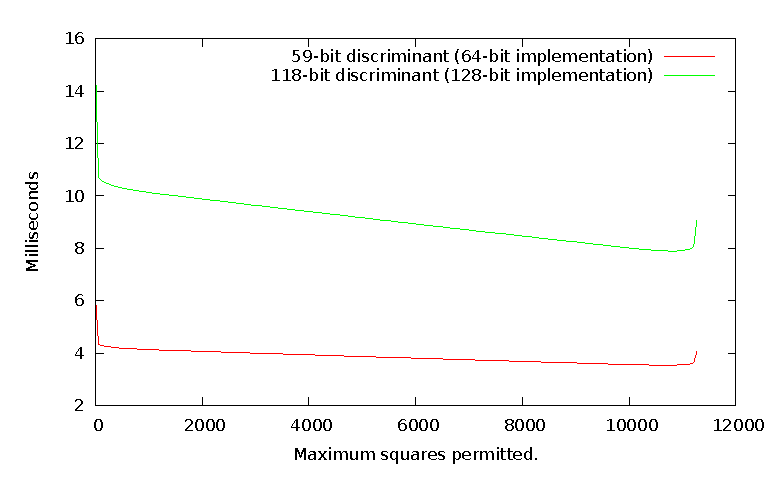
\includegraphics{dbns_l2r_vary_max}
\caption[Global bounds on left-to-right 2,3 representations.]{The time to exponentiate the $1000^{\textrm{th}}$ primorial, $n$, while varying the maximum number of squares permitted, $A$. The maximum number of cubes is $B = \ceil{\log_3(n/2^A)}$.}
\label{fig:dbnsL2rVaryBounds}
\end{figure}

In general, bounding the maximum number of squares and cubes give representations that lead to faster exponentiation in the ideal class group than representations where the number of squares or cubes is left unbound.  For this particular exponent, a representation generated without a global bound takes approximately 7.3 milliseconds for a 59-bit discriminant and 17.2 milliseconds for a 118-bit discriminant.  This is slower than all bounded representations for both implementations.

\section{Greedy Pruned Trees}

% This is also a contribution.  See the $L$ best approximations section for more info.

A right-to-left 2,3 chain can be generated by repeatedly reducing the exponent by 2 and 3 and then either adding or subtracting 1 and repeating this process until the exponent is 1.  In the windowed variant, after reducing the exponent by 2 and 3, we had 12 residues modulo $2^2 3^2$ and this lead to $2^{12}$ different strategies for adding or subtracting 1 from the residue.

In Subsection \ref{subsec:pm1Tree}, we discussed a tree based method where a set of at most $L$ \emph{partial representations} are maintained (a partial representation can be written as $n = x + \sum s_i2^{a_i}3^{b_i}$).  At each iteration, the $x$ term from each partial representation generates two new elements $x-1$ and $x+1$.  After reducing each new element by powers of 2 and 3, only the $L$ smallest are kept.  More formally, an element $x$ generates new integral elements $(x \pm 1)/(2^c3^d)$.

Here we consider two variations to the approach of maintaining the $L$ best\footnote{We say that a partial representation is \emph{better} when the $x$ term is smaller, or if the $x$ terms are equal, when the cost of the 2,3 summation is less.} partial representations. The first variation we consider is to generate several new nodes with integer values of the form $(x \pm 2^a3^b)/(2^c3^d)$, while the second variation is to include two terms such that each node generates values of the form $(x \pm 2^a \pm 3^b) / (2^c 3^d)$.  Notice that the first variation includes the forms $(x \pm 1)/(2^c 3^d)$ and so tends to give representations no worse than the method suggested by Doche and Habsieger \cite{Doche2008} (covered in Subsection \ref{subsec:pm1Tree}).  The assumption is that by adjusting $x$ by more than just 1, we increase the likelihood of finding a multiple of a large $2^c3^d$ window.

\mygraphTwoX{pm2a3b_vary_max-64}{pm2a3b_vary_max-128}{fig:pm2a3bVaryMax}{Performance of varying the bounds $a, b \le U$ on $(x \pm 2^a3^b)/(2^c3^d)$ when exponentiating by the primorial $P_{1000}$.}{Global bounds on $(x \pm 2^a3^b)/(2^c3^d)$.}
For both variations, we bound $a$ and $b$ such that $0 \le a \le U$ and $0 \le b \le U$.  Figure \ref{fig:pm2a3bVaryMax} shows the average time to exponentiate by the $1000^{\textrm{th}}$ primorial as the bound $U$ increases (using the $k=4$ best partial representations).  As $U$ increases, computing representations using this approach quickly becomes intractable.  We found that for our purposes, $U=16$ is an acceptable trade off between the average time to exponentiate and the time to generate the 2,3 representation.


\section{The $L$ Best Approximations}
\label{sec:expBestApproximations}

% TODO: State that we came up with this method.
% In this section, we introduce a novel method for exponentiation that we call L best approximations."  Follow this with some motivation, including things like
% - reason/motivation for developing the new method
% - derivation (eg. is this a proposed/suggested improvement over an existing method)
% - what was the main idea behind the method, improvements
% - does it actually yield improvements in practice

% I can't remember whether this was the method of choice for any parameter sizes.  If it is, you need to include mention of your original method in the intro to the exponentiation chapter, as well as in Ch 1 when describing your contributions.  Otherwise, you describe it as an attempt to improve that was tried, but unfortunately didn't help in practice.


The approach of maintaining a set of the $L$ best partial representations of an exponent can be adapted to that of the left-to-right 2,3 representation from Subsections \ref{subsec:ltorChains} and \ref{sec:ltorChains2}.  For an integer $x$ we say that $2^a3^b$ is a best approximation of $|x|$ when $\left||x| - 2^a3^b \right|$ is minimal.  The algorithm for the left-to-right representation (Subsection \ref{subsec:ltorChains}) finds a best approximation for $x$ and then repeats on the positive difference. However, instead of only iterating on the best approximation, each value from the set of partial representations generates new values of the form $\left||x| - 2^a3^b\right|$ (being careful to record the sign of $x$), and the $L$ best partial representations are retained.  In this case, we iterate $b$ from $0 \le b \le B$ and let $a_1 = \floor{\log_2 (x/3^b)}$ and $a_2 = \ceil{\log_2 (x/3^b)}$ bounding both $a_1, a_2 \le A$.  Note that using $a_2 = a_1 + 1$ is sufficient since either $\ceil{\log_2 (x/3^b)} = \floor{\log_2 (x/3^b)}$ or $\ceil{\log_2 (x/3^b)} = \floor{\log_2 (x/3^b)} + 1$.  We then use $\left||x|-2^{a_1}3^b\right|$ and $\left||x|-2^{a_2}3^b\right|$ as candidates for the new set.  As before, iterating the bound on the number of squares and cubes varies the cost of the representations generated.  


\section{Additive 2,3 Chains}

% Small contribution here.

Imbert and Philippe \cite{Imbert2010b} give a method (see Subsection \ref{subsec:shortAddChains}) to compute the shortest additive strictly chained 2,3 partition, suitable for smaller integers.  Such partitions do not permit subtraction and every term is strictly less than and divides all subsequent terms. They take the form
\[
	n = \sum_{i=0}^k 2^{a_i}3^{b_i}
\]
for $a_i, b_i \in \ZZgez$ where $2^{a_i}3^{b_i}$ divides $2^{a_j}3^{b_j}$ and $a_i < a_j$ and $b_i < b_j$ for all $i < j$.

For our purposes, we modified this algorithm to compute additive 2,3 chains that minimize the average cost of arithmetic in the ideal class group -- the resulting additive 2,3 chains give a better average time for exponentiation, while they are not necessarily the shortest possible.  

Let $M$, $S$, and $C$ be the average cost to multiply, square, and cube respectively. Our modified function is as follows
\begin{equation*}
s'(n) = \begin{cases}
	\min\{S + s'(n/2), C + s'(n/3)\} & \textrm{when } n \equiv 0 \pmod 6 \\
	M + s'(n-1) & \textrm{when } n \equiv 1 \pmod 6 \\
	S + s'(n/2) & \textrm{when } n \equiv 2 \pmod 6 \\
	\min\{C + s'(n/3), M + S + s'((n-1)/2)\} & \textrm{when } n \equiv 3 \pmod 6 \\
	\min\{S + s'(n/2), M + C + s'((n-1)/3)\} & \textrm{when } n \equiv 4 \pmod 6 \\
	M + S + s'((n-1)/2) & \textrm{when } n \equiv 5 \pmod 6
\end{cases}
\end{equation*}
where $s'(1) = 0$, $s'(2) = S$, and $s'(3) = C$ are the base cases.

We also experimented with computing 2,3 strictly chained partitions that allow for both positive and negative terms.  The corresponding function we used is
\begin{equation*}
f(n) = \begin{cases}
	\min\{S + f(n/2), C + f(n/3)\} & \textrm{when } n \equiv 0 \pmod 6 \\
	\min\{M + f(n-1), M + S + f((n+1)/2)\} & \textrm{when } n \equiv 1 \pmod 6 \\
	\min\{S + f(n/2), M + C + f((n+1)/3)\} & \textrm{when } n \equiv 2 \pmod 6 \\
	\begin{split}\min\{C + f(n/3), M + S + f((n-1)/2),\\M + S + f((n+1)/2)\}\end{split} & \textrm{when } n \equiv 3 \pmod 6 \\
	\min\{S + f(n/2), M + C + f((n-1)/3)\} & \textrm{when } n \equiv 4 \pmod 6 \\
	\min\{M + f(n+1), M + S + f((n-1)/2)\} & \textrm{when } n \equiv 5 \pmod 6 \\
\end{cases}
\end{equation*}
again, where $f(1) = 0$, $f(2) = S$, and $f(3) = C$ are the base cases.  One thing to notice is that the function $s'$ computes a subset of the representations computed by the function $f$.  As such, we expect the average cost to exponentiate using a representation computed by $f$ to be no worse than the average cost to exponentiate using a representation computed by $s$.

\section{Incremental Searching}

% This is also a contribution.

For small inputs, the number of additive 2,3 chains is sufficiently reduced that we can compute all such chains in order to find the fastest.  Here we consider a different approach to searching for representations -- for a function generating a set of representations, we record the cheapest representation for each integer represented by the set.

We first iterate over all single term representations $2^{a_1}3^{b_1}$ for $0 \le a_1 \le A$ and $0 \le b_1 \le B$, and then all two term representations $2^{a_1}3^{b_1} \pm 2^{a_2}3^{b_2}$ for $0 \le a_1 < a_2 \le A$ and $0 \le b_1 < b_2 \le B$.  In general, we compute the set of representations
\[
R = R_1 \cup R_2 \cup ... \cup R_m
\]
for some maximum number of terms $m$ where
\[
R_k = \left\{\sum_{i=1}^k\pm 2^{a_i}3^{b_i} ~:~ 0 \le a_1 < \cdots < a_k \le A \textrm{ and } 0 \le b_1 < \cdots < b_k \le B \right\}.
\]
We iterate over the set $R$ and for each integer represented, we record the lowest cost representation for that integer in $R$.

In our experiments, we search for representations for 16-bit integers. We initially chose $A = \ceil{\log_2\left(2^{16}\right)} = 16$, $B = \ceil{\log_3 \left(2^{16}\right)} = 11$, and iterated the number of terms $k$ from 1 through 5. For representations of $k = 6$ terms, our implementation did not complete after a week of execution.  We then ran our search again using $A=18$ and $B=12$ and found that none of our minimal representations were improved.

Since both the incremental search of this section and the two functions from the previous section are computationally expensive, we are only able to compute chains for small exponents.  This is still useful when we consider methods that partition large exponents into smaller blocks using their binary representation, or when we consider multiple exponentiations by a list of prime powers.


\section{Big Exponents from Small Exponents}

The techniques of the previous two sections are computationally expensive and as such, we limit our search to representations of 16-bit integers.  One way that we use such representations is to write the exponent $n$ in 16-bit blocks as
\[
	n = \sum_{i=0}^k 2^{16i} b_i
\]
where $0 \le b_i < 2^{16}$.  Assuming that we can exponentiate a group element $g$ to a 16-bit exponent $b_i$, Algorithm \ref{alg:blockedExp} computes the exponentiation $g^n$ using an approach similar to a left-to-right windowed binary exponentiation.

\begin{algorithm}[htb]
\caption{16-bit Blocked Exponentiation.}
\label{alg:blockedExp}
\begin{algorithmic}[1]
\Require $n \in \ZZ, g \in G$ and a method to compute $g^{b_i}$ for $0 \le b_i < 2^{16}$.
\Ensure $g^n$
\State $R \gets 1_G$
\For {$i$ from $\ceil{\log_{2^{16}} n}$ downto 0}
	\State $R \gets R^{2^{16}}$ \Comment{By repeated squaring.}
	\State $b_i \gets \floor{n / 2^{16i}} \bmod {2^{16}}$
	\State $R \gets R \cdot g^{b_i}$ \Comment{Externally compute $g^{b_i}$.}
\EndFor
\State \Return $R$
\end{algorithmic}
\end{algorithm}

Another way we can use 16-bit representations is when we know the prime factorization of the exponent $n$ and $n$ is the product of primes smaller than $2^{16}$.  Since we are interested in exponentiation by primorials (i.e.\ the product of the first $w$ primes), the prime factorization is trivial. Given a primorial $P_w = \prod_{i=1}^w p_i$ where $p_i$ is the $i^{\textrm{th}}$ prime, we can compute $g^{P_w}$ as $(((g^{p_1})^{p_2})^{\cdots})^{p_w}$ using a series of $w$ small exponentiations.

\section{Experimental Results}
\label{sec:expResults}

One reason to improve the performance of exponentiation in the ideal class group is to improve the performance of order finding in this group.  In particular, we exponentiate a random ideal class to a primorial so that the order of the resulting ideal class is likely to be coprime to our exponent.

Two of the techniques in the previous section compute $g^n$ using a series of smaller exponentiations $g^b$ such that $0 \le b < 2^{16}$.  So we begin by determining the best method to exponentiate using 16-bit exponents.  To do so, we compute the average time to exponentiate for exponents 1 through 65535 using 59-bit and 118-bit discriminants.  Table \ref{tab:exp16bitWinners} shows the number of exponents for which each method was the fastest\footnote{The methods not listed in this table were not the fastest for any exponents.}.
\begin{table}[htb]
\centering
\begin{tabular}{| l | r | r |}
	\hline
	Method & 59-bit Discriminants & 118-bit Discriminants \\
	\hline
	Left-to-Right 2,3 Representation & 2536 & 7097 \\
	4 Best $\left||x|-2^a3^b\right|$ & 9091 & 7230 \\
	4 Best $(x \pm 2^a3^b)/(2^c3^d)$ & 47969 & 45468 \\
	4 Best $(x \pm 2^a \pm 3^b)/(2^c3^c)$ & 3333 & 2756 \\
	Recursive $\sum 2^a3^b$ Chains & 2406 & 2970 \\
	Incremental Search & 199 & 13 \\
	\hline
\end{tabular}
\caption[Best 16-bit exponentiation techniques.]{The number of 16-bit exponents where an exponentiation technique was fastest.}
\label{tab:exp16bitWinners}
\end{table}
For each exponent, we then normalized the time of each method relative to the best time.  Table \ref{tab:exp16bitTimes} shows the average of these normalized times.
\begin{table}[htb]
\centering
\begin{tabular}{| l | c | c |}
	\hline
	Method & 59-bit Discriminants & 118-bit Discriminants \\
	\hline
	Binary & 1.48864 & 1.44287 \\
	Right-to-Left Non-Adjacent Form & 1.39605 & 1.34547 \\
	Right-to-Left 2,3 Chain & 1.35869 & 1.37595 \\
	$2^2 3^2$ Windowed Right-to-Left 2,3 Chain & 1.38676 & 1.37415 \\
	Left-to-Right 2,3 Representation & 1.27775 & 1.23781 \\
	4 Best $\left||x|-2^a3^b\right|$ & 1.19508 & 1.17034 \\
	4 Best $(x \pm 1)/(2^c3^d)$ & 1.23152 & 1.22800 \\
	4 Best $(x \pm 2^a3^b)/(2^c3^d)$ & 1.03227 & 1.03886 \\
	4 Best $(x \pm 2^a \pm 3^b)/(2^c3^c)$ & 1.37963 & 1.38966 \\
	Recursive $\sum 2^a3^b$ Chains & 1.28606 & 1.26822 \\
	Recursive $\sum \pm 2^a3^b$ Chains & 1.21295 & 1.18712 \\
	Incremental Search & 1.19495 & 1.17059 \\
	\hline
\end{tabular}
\caption{Normalized time to exponentiate 16-bit exponents.}
\label{tab:exp16bitTimes}
\end{table}
The method that maintains the 4 best partial representations of the form $(x \pm 2^a3^b)/(2^c3^d)$ was the best performer in general.  However, since we were interested in precomputing 16-bit representations for use with a block exponentiation and exponentiation by a list of prime factors, we used the best representation available for each exponent.

To determine the best method to exponentiate a random ideal by a primorial, we compute the average time to exponentiate for the primorials $P_{250k}$ for $1 \le k \le 100$.  We categorized the different exponentiation techniques as those that use only base 2, those that generate 2,3 chains from right-to-left, from left-to-right, that add or subtract to a partial representation and then reduce by $2^c3^d$, and those that make use of the best 16-bit representations.  We then compared the average time to exponentiate each method from a category, and finally compared the best performers of each category to determine the best performer overall.

We found that for both our 64-bit and 128-bit implementations and for all primorials tested, the method of iterating on the 4 best $\left||x| - 2^a3^b\right|$ approximations leads to representations with the fastest time to exponentiate.  This is in contrast to the method of iterating on the 4 best partial representations $(x \pm 2^a3^b)/(2^c3^d)$ that lead to the best timings for 16-bit integers.  Naturally, we can improve these results by iterating on the $L$ best partial representations for $L > 4$ at the expense of longer precomputation.

Figures \ref{fig:expBinNaf64} and \ref{fig:expBinNaf128} compare binary exponentiation against right-to-left non-adjacent form representation.  The non-adjacent form representation leads to faster exponentiations in all cases.  Figures \ref{fig:expDbnsR2L64} and \ref{fig:expDbnsR2L128} compare the non-windowed right-to-left 2,3 chain method to the $2^2 3^2$ windowed method.  The $2^23^2$ windowed method out performs the non-windowed method for all exponents.  Figures \ref{fig:expDbnsL2R64} and \ref{fig:expDbnsL2R128} compare left-to-right 2,3 representations with that of maintaining the 4 best $\left||x|-2^a3^b\right|$ approximations.  In this case, maintaining the 4 best approximations performs best.  Figures \ref{fig:expPmVariants64} and \ref{fig:expPmVariants128} compare the three different techniques of adding or subtracting a value to a partial representation and then reducing by a power of 2 and 3.  Here, computing candidates $(x-2^a3^b)/(2^c3^d)$ leads to representations that exponentiate the fastest.  Figures \ref{fig:expBlockList64} and \ref{fig:expBlockList128} compare the two methods that rely on the best found 16-bit representations.  In this case, when the factorization of the exponent is easily known, it is faster to exponentiation by the list of prime factors than it is to represent the exponent using 16-bit blocks.  Finally, Figures \ref{fig:expWinners64} and \ref{fig:expWinners128} compare the best performer from each category.

\mygraph{binary_vs_naf-64}{fig:expBinNaf64}{Base 2 Exponentiation (59-bit Discriminants).}
\mygraph{binary_vs_naf-128}{fig:expBinNaf128}{Base 2 Exponentiation (118-bit Discriminants).}

\mygraph{dbns_r2ls-64}{fig:expDbnsR2L64}{Right-to-Left 2,3 Chains (59-bit Discriminants).}
\mygraph{dbns_r2ls-128}{fig:expDbnsR2L128}{Right-to-Left 2,3 Chains (118-bit Discriminants).}

\mygraphTwo{dbns_l2rs-64}{dbns_l2rs-64-zoom}{fig:expDbnsL2R64}{Left-to-Right 2,3 Representations (59-bit Discriminants).}
\mygraphTwo{dbns_l2rs-128}{dbns_l2rs-128-zoom}{fig:expDbnsL2R128}{Left-to-Right 2,3 Representations (118-bit Discriminants).}

\mygraphTwo{pm_variants-64}{pm_variants-64-zoom}{fig:expPmVariants64}{4 Best $(x\pm\cdots)/(2^c3^d)$ (59-bit Discriminants).}
\mygraphTwo{pm_variants-128}{pm_variants-128-zoom}{fig:expPmVariants128}{4 Best $(x\pm\cdots)/(2^c3^d)$ (118-bit Discriminants).}

\mygraph{block_vs_list-64}{fig:expBlockList64}{Use $g^b$ for 16-bit $b$ (59-bit Discriminants).}
\mygraph{block_vs_list-128}{fig:expBlockList128}{Use $g^b$ for 16-bit $b$ (118-bit Discriminants).}

\mygraph{winners-64}{fig:expWinners64}{The best performers from each category (59-bit Discriminants).}
\mygraph{winners-128}{fig:expWinners128}{The best performers from each category (118-bit Discriminants).}


\section{Summary}

This chapter presented the approach and results used to improve exponentiation in the ideal class group of imaginary quadratic number fields.  Several methods for exponentiation including novel extensions to methods for computing 2,3 chains and representations were explored.  We found that for 16-bit exponents, the method of iterating on the $L$ best partial representations $x + \sum s_i2^{a_i}3^{b_i}$ such that each $x$ generates new terms of the form $(x \pm 2^a 3^b)/(2^c3^d) \in \ZZ$ gives the fastest representation on average.  For large primorial exponents, generating new terms of the form $\left||x|-2^a3^b\right|$ gave the fastest representations on average.

The next chapter brings together the improvements to ideal arithmetic and exponentiation in our implementation of SuperSPAR -- an algorithm with the fastest average time to factor integers $n$ in the range $2^{54} \le n < 2^{63}$ of the integer factoring algorithms that we tested.



%%%%%%%%%%%%%%%%%%%%%%%%%
% SUPERSPAR EXPERIMENTS %
%%%%%%%%%%%%%%%%%%%%%%%%%
\chapter{SuperSPAR Experiments}
\label{chap:ssparExperiments}

The goal of this chapter is to demonstrate that the SPAR integer factoring algorithm (Section \ref{sec:spar}) can be modified and implemented so that, on average, it is the fastest available factoring implementation for integers of the size 50-bits to 62-bits -- this is an implementation of SuperSPAR (Section \ref{sec:superSpar}).  One way in which factoring integers of these sizes is useful is after the sieve step of more powerful integer factoring algorithms, such as the number field sieve (see \cite[\S 6.2]{Crandall2001}).  Factoring integers of these sizes is also of particular interest in this thesis since Chapter \ref{chap:xgcdExperiments} demonstrates performance improvements on average for computing the extended GCD using our 32-bit, 64-bit, and 128-bit implementations, while Chapter \ref{chap:idealExperiments} demonstrates performance improvements on average for ideal class group arithmetic for orders with discriminant no larger than 118-bits.  This is relevant to our implementation of SuperSPAR, since SuperSPAR is based on the SPAR factoring algorithm (discussed in Section \ref{sec:spar}), which is based on arithmetic in the ideal class group.

SPAR factors an integer $N$ by attempting to compute the order of a random ideal class in an order with discriminant $\Delta = -kN$ for some square free integer $k$.  An implementation first exponentiates a random ideal class to the product of many small primes (the exponentiation stage) and then performs a random walk in an attempt to find an ambiguous ideal class (the search stage).  Our implementation of SuperSPAR improves upon the search stage of SPAR by using a bounded primorial steps search, due to Sutherland \cite{Sutherland2007} and discussed in Subsection \ref{subsec:boundedPrimorialSteps}.  This is a practical improvement over a random walk search since a bounded primorial steps search has an asymptotically faster worst case (see Subsection \ref{subsec:boundedPrimorialSteps}), which means that it requires fewer group operations to find the order of an ideal class.

Our implementation of SuperSPAR also improves upon the exponentiation stage of SPAR.  In this stage, SPAR exponentiates a random ideal class to the product of many small primes.  Since our implementations of ideal class arithmetic include cubing, we take advantage of 2,3 representations for exponentiation, which is an improvement over binary exponentiation (see Section \ref{sec:expResults}).  For SuperSPAR, we precompute 2,3 representations using the $L$ best approximations technique of Section \ref{sec:expBestApproximations}, which Chapter \ref{chap:powExperiments} shows to perform the best on average for large exponents that are the product of many primes and for ideal classes for orders with discriminants no larger than 118-bits.

Another way in which our implementation of SuperSPAR improves upon SPAR is by bounding the number of group operations used by each stage independently from each other and separate from the theoretically optimal values.  In SPAR, each stage uses $O(p_t)$ group operations where $p_t \approx N^{1/2r}$ and $r = \sqrt{\ln N / \ln \ln N}$ (see Subsection \ref{subsec:sparAlg} for additional details).  The value for $r$ is chosen to theoretically minimize the expected running time of the algorithm, since the assumption is that the order of a random ideal class $\aclass \in Cl_\Delta$ with $\Delta = -kN$ is $N^{1/2r}$ smooth with probability $r^{-r}$.  In practice, other values of $p_t$ are more efficient.  

Furthermore, balancing both stages to use $O(p_t)$ group operations is not ideal.  This is partly because the actual cost of multiplication, squaring, and cubing differ, but also because the success of each stage depends on different properties of the class number.  The exponentiation stage is successful when the order of a random ideal class is smooth with respect to the exponent $E$ used in the exponentiation stage, while the search stage is successful when the non-smooth part of the order is sufficiently small.  Selecting bounds for each stage independently of $r$ varies the time spent during each stage inversely to the probability of its success.  As such, our implementation of SuperSPAR selects the largest prime $p_t$, used in the exponent $E = \prod {p_i}^{e_i}$ in the exponentiation stage, separately from the multiple of a primorial, $mP_w$, used in the search stage.  Note that the largest prime $p_t$ used during the exponentiation stage is larger than the largest prime $p_w$ used by the search stage, since the search stage assumes that the order of $\bclass = \aclass^E$ is coprime to $E$.

In addition to allowing the largest prime $p_t$ used in the exponent $E = \prod {p_i}^{e_i}$ to differ from the theoretically optimal value, we also bound the prime exponents $e_i$ differently from the theoretical values suggested by Schnorr and Lenstra, who incidentally advise the use of smaller exponents in practice (see \cite[p.293]{Schnorr1984} and Subsection \ref{subsec:ssparPrimePowerBound} of this thesis).

Since there are several parameters affecting the performance of our implementation of SuperSPAR, we first say a little about the methodology used in this chapter.  This chapter, like previous chapters, emphasizes empirical results, however, factoring a single integer is considerably slower than computing a single extended GCD or performing a single arithmetic operation in the ideal class group.  In the case of computing the extended GCD, a single computation takes on average between a few nanoseconds to a few hundred nanoseconds.  This means that we can empirically test 1,000,000 computations for random integers of each size from 1-bit to 127-bits in a modest amount of time.  Even for ideal class arithmetic, multiplication, squaring, and cubing take between a few hundred nanoseconds to a few microseconds.  Again, because of this we are able to empirically time each operation on 10,000,000 random ideal classes for discriminants of size 16-bits to 140-bits in a few hours.  On the other hand, factoring a single integer with our implementation of SuperSPAR takes less than 100 microseconds on average for properly chosen parameters for 32-bit integers, but over 50 milliseconds on average for poorly chosen parameters for 100-bit integers -- this is roughly between 10,000 times to 500,000 times slower than an extended GCD computation.  So even for small sets of integers (a few 1000), this is quite slow and may not lead to parameters that work well on average.

To aid in the selection of efficient parameters for our implementation of SuperSPAR, Section \ref{sec:ssparFactorizationOfTheOrder} discusses the statistical analysis of a set of roughly 6,000,000 ideal classes in order to find bounds on several parameters.  Subsection \ref{subsec:ssparPrimePowerBound} shows that the prime factorization of the order of ideal classes consists of prime powers with exponents that are typically 1 for all but the smallest primes.  This informs the value of each $e_i$ in the exponent $E$ for the exponentiation stage.  Additionally, we found that the order of an ideal class $[\ideal a_1]$ was, with high probability (about 97.8\% in our experiments), either the same as or a multiple of the order of some other ideal class $[\mathfrak a_2]$ in the same class group (see Subsection~\ref{subsec:ssparDiffBtwOrder}).  For this reason, if the algorithm finds some $h'$ such that ${[\mathfrak a_1]^{h'}}^{\left(2^j\right)}$ is an ambiguous class for some $j$, but is unsuccessful at factoring $N$, the algorithm simply attempts to find an ambiguous class by repeated squaring of $[\mathfrak a_i]^{h'}$ for several $[\mathfrak a_i]$.  Since this may fail for several ideal classes, we let $c$ be the maximum number of ideal class classes tried before the algorithm starts over with a different multiplier $k$ for the discriminant.  Although the statistical data shows that in expectation a value of $c \approx 2$ is all that is needed (see Subsection \ref{subsec:ssparExpIdeals}), we rely on empirical testing to show that much larger values of $c$ perform better in practice.  Similarly, the largest prime $p_t$ used in the exponent $E$ for the exponentiation stage, and the multiple of a primorial $mP_w$ used for the search stage are determined empirically in Section \ref{sec:ssparEmpirical}.

The software used to generate timing information was developed using \compiler{} on 64-bit Ubuntu 12.10.  Assembly language was used for 128-bit arithmetic on x64 processors and for processor specific features.  The C programming language was used for all other implementation details.  The CPU is a \cpu{} with 8Gb of RAM and has four cores, only one of which was used for timing experiments.  Unless otherwise specified, the timings associated with factoring integers are the average time to factor one integer from a set of 4,000 semiprime integers, such that each integer is the product of two primes of equal size.  All empirical timings for integers of a given size use the same set of 4,000 semiprime integers.

Exponents used for the exponentiation stage were precomputed using the $L$ best approximations technique from Section \ref{sec:expBestApproximations}, which Chapter \ref{chap:powExperiments} shows performs the fastest for exponents that are the products of many small primes and for our implementations of ideal class group arithmetic.  The implementation of ideal class arithmetic used is that discussed in Chapter \ref{chap:idealExperiments}, specifically, we use the 64-bit implementation for all class groups with discriminant no larger than 59-bits, and we use the 128-bit implementation for class group with discriminant larger than 59-bits, but no larger than 118-bits.  Our implementation of SuperSPAR will work for integers larger than 118-bits, however, empirical tests show that SuperSPAR was not competitive for larger integers.   Extended GCD computations used for ideal arithmetic are based on the results of Chapter \ref{chap:xgcdExperiments}.  For an ideal $\ideal a = [a, (b + \sqrt\Delta)/2]$, the coefficients $a$ and $b$ are roughly half the size of the discriminant $\Delta$.  As such, our 64-bit implementation of ideal arithmetic favours our 32-bit implementations of the extended Euclidean algorithm, however, when arguments are larger than 32-bits, our implementation uses our 64-bit implementations of our simplified left-to-right binary extended GCDs.  Our 128-bit implementation of ideal arithmetic favours of 64-bit implementations of our simplified left-to-right binary extended GCDs, but similarly, when arguments are larger than 64-bits, our implementation uses our 128-bit implementation of Lehmer's extended GCD using our 64-bit simplified left-to-right binary extended GCD for 64-bit machine words.   In each case, when a left-only or partial extended GCD is needed, our implementation uses the left-only or partial implementation of the corresponding full extended GCD.  Our GMP implementation of ideal arithmetic is not utilized during these tests since our implementation of SuperSPAR was not competitive for integers larger than 118-bits, which is the largest size supported by our 128-bit implementation of ideal class arithmetic.

The sections in this chapter are as follows.  Section \ref{sec:ssparCoprimeFinding} discusses two techniques to generate a list of integers (or deltas between integers) coprime to a primorial up to a given bound.  This is useful during the search stage of SuperSPAR when we take baby steps coprime to the multiple of a primorial $mP_w$.  The search stage requires the use of a lookup table.  Section \ref{sec:ssparHashing} discusses how our implementation hashes an ideal class and then compares two methods of resolving hash collisions, namely chaining with list heads and open addressing.  Open addressing performs faster on average.  As discussed in Subsection \ref{subsec:boundedPrimorialSteps}, for the search stage to work, the order of the element should have no factors in common with the primorial used for the search stage.  Section \ref{sec:ssparFactorizationOfTheOrder} discusses the data and experiments used to bound the exponents of the prime factors of the exponent used in the exponentiation stage so that (with high probability) the order of the resulting ideal class will have no factors in common with the primorial used during the search stage.  This section also discusses the number of ideal classes to try in expectation for a given class group.  To enable the discovery of bounds useful for the search stage, Section \ref{sec:ssparBabyStepBounds} discusses a method of generating suitable candidates.  With all this in place, Section \ref{sec:ssparEmpirical} discusses the method we use to determine the exponent for the exponentiation stage and the bound for the search stage that work well in practice for integers of specific sizes.  Finally, a comparison of our implementation of SuperSPAR to several public implementations of factoring algorithms is provided.  We show that for pseudorandom semiprime integers between 50-bits and 62-bits inclusive, SuperSPAR performs the best on average of the implementations tested.


\section{Coprime Finding}
\label{sec:ssparCoprimeFinding}

% TODO: State our coprime wheel as a contribution.

The bounded primorial steps algorithm from Subsection \ref{subsec:boundedPrimorialSteps} and adapted by the SuperSPAR factoring algorithm (Section \ref{sec:superSpar}) computes baby-steps $\aclass^i$ for $1 \le i \le s$ where $i$ is coprime to some primorial $P_w$ and $s$ is a multiple of $P_w$.  By considering only values coprime to $P_w$ the running time complexity of the bounded primorial steps algorithm achieves an upper bound of $O(\sqrt{M/\log \log M})$ group operations in the worst case.  If an implementation has to test whether each $i$ from $1$ to $P_w$ is coprime to $P_w$, the algorithm cannot achieve this.  As such, the algorithm assumes a set of values coprime to $P_w$ is globally available.  Of course, one can generate such a set by testing whether $\gcd(i, P_w) = 1$ for $i$ from $1$ to $P_w$, but there are more efficient methods.  This section discusses two such methods, namely sieving and wheeling.  Additional information on each technique can be found in \cite[pp.117--127]{Crandall2001} and \cite[p.494]{Sutherland2009}.

\subsection{Coprime Sieve}

Sieving the values coprime to some primorial $P_w$ is straightforward since the factorization $P_w = 2 \times 3 \times \cdots \times p_w$ is known.  Let $[1,b]$ denote the range to be sieved.  First, create a table mapping the values $1$ through $b$ to \emph{true}.  Then for each prime factor $p_j$ of $P_w$, and for every multiple $mp_j$ such that $1 \le mp_j \le b$, set the table entry at index $mp_j$ to \emph{false}.  At this point, each index with a \emph{true} value is coprime to $P_w$.  To see this, note that an index $x$ is \emph{false} when there was some multiple $m$ of a prime $p_j$ dividing $P_w$ such that $mp_j = x$.  As such, the value of $x$ is false if and only if $x$ and $P_w$ share a common factor, namely $p_j$.

\subsection{Coprime Wheel}
\newcommand{\coprimeset}{\set C}
\newcommand{\coprimelist}{\set D}

When the value $b$ from the previous section is equal to the primorial $P_w$, a coprime wheel may be faster in practice.  First, suppose that for some primorial $P_w$, the set of all integers $1 \le x < P_w$ coprime to $P_w$ is already known.  More formally, let
\[
	\coprimeset_w = \left\{x : \gcd(x, P_w) = 1, 1 \le x < P_w \right\}.
\]
As such, there is no $x \in \coprimeset_w$ that is divisible by any prime $p_j$ that divides $P_w$.  The values $x + mP_w$ for $x \in \coprimeset_w$ and $m \in \ZZ$ are also coprime to $P_w$, and so act as a set of representatives of the integers modulo $P_w$ that are coprime to $P_w$.  Let $\coprimeset_w + mP_w$ denote the set $\{x + mP_w : x \in \coprimeset_w\}$.  Computing
\[
	\bigcup_{0 \le m < p_{w+1}} \coprimeset_w + mP_w
\]
generates the set of all positive integers less than $P_{w+1}$ that are coprime to $P_w$.  Removing all multiples of $p_{w+1}$ from this set implies that no element is divisible by a prime $p_j \le p_{w+1}$.  As such, the set
\[
	\coprimeset_{w+1} =
		\left( \bigcup_{0 \le m < p_{w+1}} \coprimeset_w + mP_w \right)
	    \setminus \{ m' p_{w+1} : 1 \le m' < P_w \}
\]
is the set of all values $1 \le x < P_{w+1}$ that are coprime to $P_{w+1}$.

The primorial $P_1 = 2$ has the set $\coprimeset_1 = \{1\}$ of integers coprime to 2.  This acts as a base case, from which the representative set of integers coprime to primorials $P_2, P_3, ..., P_w$ are computed by recursive application of the above steps.

Our implementation of SuperSPAR iterates baby steps for consecutive integers coprime to some primorial $P_w$.  As such, the difference between coprime integers is used instead, and the above technique is adapted to work with lists of deltas between consecutive coprime integers.  Each list begins with the difference from the first coprime integer 1 (which is coprime to all integers) to the next integer coprime to some primorial $P_w$. Let
\[
	\coprimelist_w = d_1, ..., d_{\phi(P_w)}
\]
such that $d_i = c_{i+1} - c_i$ for consecutive integers $c_i$ and $c_{i+1}$ coprime to $P_w$ where $c_1 = 1$. The list $\coprimelist_1$ consists of the single value 2.

\begin{algorithm}[htb]
\caption{Compute deltas for $P_{w+1}$ given deltas for $P_w$.}
\label{alg:deltaWheel}
\begin{algorithmic}[1]
\Require A primorial $P_w$, the delta list $\coprimelist_w$, and the next prime $p_{w+1}$.
\algnewline Let $P_{w+1} = p_{w+1} P_w$ and $\phi(P_{w+1}) = (p_{w+1}-1)\phi(P_w)$.
\Ensure The delta list $\coprimelist_{w+1}$.
\State $i \gets 1, j \gets 1, c \gets 1, d \gets 0$
\While{$j \le \phi(P_{w+1})$}
	\State $c \gets c + d_i$ \Comment{each $c$ is coprime to $P_w$}
	\State $d \gets d + d_i$
	\If{$c \not\equiv 0 \pmod{p_{w+1}}$}
		\State $d'_j \gets d, d \gets 0, j \gets j + 1$ \Comment{output $d$ when $c$ is coprime to $P_{w+1}$}
	\EndIf
	\State $i \gets i + 1$
	\If{$i > \phi(P_w)$}
		\State $i \gets 1$
	\EndIf
\EndWhile
\State \Return $d'_1, ..., d'_{\phi(P_{w+1})}$
\end{algorithmic}
\end{algorithm}

Algorithm \ref{alg:deltaWheel} computes $\coprimelist_{w+1}$ given $\coprimelist_w$, $P_w$, and the next prime $p_{w+1}$.  The algorithm starts with the current candidate integer, $c$, coprime to $P_{w+1}$ and a delta counter $d = 0$.  The algorithm cycles through the delta list $\coprimelist_w$ adding each element encountered to $c$.  On each iteration, if $c$ is not a multiple of $p_{w+1}$, then the delta counter $d$ is appended to the output list $\coprimelist_{w+1}$ and then set to 0.  Otherwise, the algorithm continues with the next delta from the input list (cycling to the beginning of the list when the end is reached).  Once $\phi(P_{w+1})$ deltas have been appended to the output list, the algorithm terminates.

\subsection{Comparison}

The coprime sieve requires $b$ bits of memory, while the coprime wheel requires $\phi(P_w)$ integers for the list of deltas.  Table \ref{tab:primorialRateOfGrowth} shows the values of $\phi(P_w)$ for the first 12 primorials.  The delta list for the tenth primorial, $\phi(P_{10}) = 1021870080$, requires over a billion integers.  As such, the coprime sieve is preferred when the primorial is large, while the coprime wheel may be more efficient for large values of $b$.  This is because the coprime wheel generates deltas directly, whereas each entry in the sieve must be inspected to find integers coprime to the primorial.

\begin{table}[htb]
\centering
\begin{tabular}{| r | r | r | r |}
	\hline
	$w$ & $p_w$ & $P_w = \prod_{p \le p_w} p$ & $\phi(P_w) = \prod_{p \le p_w} (p-1)$ \\
	\hline
1 & 2 & 2 & 1 \\
2 & 3 & 6 & 2 \\
3 & 5 & 30 & 8 \\
4 & 7 & 210 & 48 \\
5 & 11 & 2310 & 480 \\
6 & 13 & 30030 & 5760 \\
7 & 17 & 510510 & 92160 \\
8 & 19 & 9699690 & 1658880 \\
9 & 23 & 223092870 & 36495360 \\
10 & 29 & 6469693230 & 1021870080 \\
11 & 31 & 200560490130 & 30656102400 \\
12 & 37 & 7420738134810 & 1103619686400 \\
	\hline
\end{tabular}
\caption{The first 12 primorials.}
\label{tab:primorialRateOfGrowth}
\end{table}

Our implementation of SuperSPAR computes baby steps coprime to a multiple of a primorial, and does so by iterating a list of deltas from one coprime value to the next.  Since this list consists of $\phi(P_w)$ integers, in practice our implementation is limited to coprime delta lists that fit within available memory, and as such to primorials $P_w$ that are not too large.  On the other hand, our implementation is still able to use much larger primorials for the exponentiation stage, since the space needed to represent a primorial is $O(\log(P_w))$ while the space needed to represent the list of coprime deltas is $O(\phi(P_w))$.  One reason we might want to use a larger primorial in the exponentiation stage is that by doing so, the order of resulting ideal class $\bclass = \aclass^E$ is likely to be coprime to $E$ and so any factors of the order of $\aclass$ that were in common with the factors of $E$ are likely to be removed by the exponentiation stage.  The order of the resulting ideal class $\bclass$ will be smaller and as such, there is a greater probability that the search stage will discover the order of the ideal class $\bclass$.  We note that the largest prime used in the exponent of the exponentiation stage can be no smaller than the largest prime in the primorial of the search stage.  If this were the case, the search stage would step coprime to a possible factor of the order of the ideal class $\aclass$ and as such, the search stage could not possible discover the order of the ideal class $\bclass$.


\section{Lookup Tables}
\label{sec:ssparHashing}

The SuperSPAR Algorithm \ref{alg:superSpar} (and more generally, the bounded primorial steps algorithm \ref{alg:primorialSteps}) requires a lookup table mapping group elements $\bclass^i$ to exponents $i$.  The baby steps generate group elements $\bclass^i$ with $i$ coprime to some primorial $P_w$ and store the mapping $\bclass^i \mapsto i$ in the lookup table. The giant steps lookup group elements $\bclass^{2js}$ and $\bclass^{-2js}$ from the lookup table.  As such, the performance of the algorithm directly corresponds to the performance of the lookup table.  This section describes the experimental results for SuperSPAR using two different implementations of lookup tables, as well as the method used to map group elements to exponents in our implementation.

Our implementation of idea class arithmetic represents an ideal class $\aclass \in Cl_\Delta$ using the triple $(a, b, c)$ where $\ideal a = [a, (b + \sqrt\Delta)/2]$ is a reduced representative for the ideal class and $c = (b^2 - \Delta)/4a$ (see Section \ref{sec:implementationOfIdealArithmetic}).  Since inversion of ideal classes is virtually free, SuperSPAR computes giant steps for ideal classes $\bclass^{2js}$ and $\bclass^{-2js}$, but rather than perform two table lookups, we take advantage of the way in which the inverse of an ideal class is computed.  Recall form Subsection \ref{subsec:idealClassInverse} that the inverse of an ideal class for a representative $[a, (b + \sqrt\Delta)/2]$ is given by the representative $[a, (-b + \sqrt\Delta)]$.  Since $|b| = \pm \sqrt{\Delta +4ac}$, we use the pair $(a, c)$ for the key and our implementation is able to look up both $\bclass^{2sj}$ and $\bclass^{-2js}$ using a single table lookup.  However, once a giant step finds a corresponding $\bclass^i$ in the table, both the exponents $2js-i$ and $2js+i$ must be tested to determine which one is a multiple of the order of $\bclass$.  Figure \ref{fig:ssparSingleLookup} contrasts this with an implementation using two lookups per giant step.  Both implementations use identical parameters on the same sets of semiprime integers, i.e.\ the executions of the two implementations only differ in the number of table lookups performed during the giant step portion of the search stage.  In the implementation using two table lookups per giant step, the pair $(a, b)$ is used for the hash key in order to distinguish between $\bclass^{2js}$ and $\bclass^{-2js}$, however, when some $\bclass^i$ is found, a multiple of the order is immediately known.

\mygraphX{hashing-single-vs-double}{fig:ssparSingleLookup}{Average time to split an integer by either using a single lookup for each giant step, with exponentiation to verify a multiple of the order, or two lookups for each giant step, but without the need to verify a multiple of the order.}{Inversion aware hashing.}

In our implementation, the lookup table is implemented as a hash table with 32-bit keys and 32-bit values (both as unsigned integers).  Our implementation maps the pair $(a, c)$ associated with an ideal class to a 32-bit hash key by computing
\[
	\hash(a, c) = (2654435761 \times (2654435761a + c)) \bmod 2^{32}.
\]
The multiplier 2654435761 was chosen because it is the largest prime less than $2^{32} \times (\sqrt 5 - 1)/2$, and $(\sqrt 5 - 1)/2$ has been shown by Knuth \cite[Section~6.4]{Knuth1998} to have good scattering properties.  Other multipliers were also tried but had little impact on performance.  Since the number of baby steps is a function of the size of the integer to be factored (see Section \ref{sec:ssparEmpirical}), the maximum number of entries in the hash table is known at initialization.  We found that a table of $2^k$ slots for the smallest $k$ such that $2^k \ge 3m\phi(P_2)$, where $m\phi(P_w)$ is the number of baby steps, worked well in practice.  Different multiples of the number of baby steps were tried, as well as setting the number of slots to a prime near some multiple of the number of baby steps.  There was little difference in performance, with the exception of a table having too few slots (resulting in an insertion failing), or a table having an excessive number of slots (in which case, table initialization dominated).  Using a power of 2 for the number of slots has the added benefit that once a hash key is computed, the corresponding slot is found by using a binary $\band$ operation.  However, regardless of the hash function used, multiple elements may hash to the same slot.  Two methods of collision resolution are considered here, each being selected for cache coherency properties (see \cite[Subsection~11.2]{Cormen2001} and \cite{Kuchling2008}).

\subsection{Chaining with List Heads}
The first method is chaining with list heads (see \cite[Subsection~11.2]{Cormen2001}).  The idea is for the hash table to consist of $2^k$ slots, such that each slot operates as a linked list, but that the head of the linked lists are separate from the tails.  Two areas of memory are used: one for the heads, and the other for the tails (also known as the overflow).  In the head, each slot consists of the 32-bit value for a specified key, as well as the 32-bit hash key itself (since multiple keys may resolve to the same slot).  A special pair of constants are used to indicate that a slot is unoccupied, e.g.\ (0xAAAAAAAA, 0x55555555).  The overflow area consists of an array of no less than $2^k$ entries, each entry consisting of the 32-bit value for a specified hash key, the 32-bit hash key itself, and an index into the overflow area of the next node in the list, if any.  A special constant, e.g.\ 0xFFFFFFFF, is used to indicate the end of list.  The first $2^k$ entries in the overflow area are reserved and correspond to the second node in the linked list of each slot.  To perform a lookup, the hash key resolves to a slot (using $\hash(a, c) \bmod 2^k$) and the list is traversed until either the specified hash key or the end of the list is found.  To insert or update, again, the list is traversed until either the specified hash key is found, at which point an update is performed, or the end of list is found.  If the end of list is found, the next available entry in the overflow area is set appropriately and appended to the end of the list. 

\subsection{Open Addressing}
The second method of collision resolution considered is open addressing, and in particular, we implement the same probing function as in CPython \cite{Kuchling2008}.  In this method, each slot consists of a 32-bit hash key, as well as the 32-bit value associated with that hash key.  Any hash key can occupy any slot, and a special pair of constants are used to indicate that a slot is unoccupied, e.g.\ (0xAAAAAAAA, 0x55555555).   When an element is hashed, the table is probed at slot indices $s_0, s_1, ...$ generated by a probing function until a slot is found where either the hash key occupying the slot is the same as the hash key for the element in question, or the slot is unoccupied.  Our implementation defines probe indices using
\begin{align*}
	s_0 &= \hash(a,b) \bmod 2^k \\
	s_i &= \left( 5s_{i-1} + 1 + \floor{\hash(a,b)/2^{5i}} \right) \bmod 2^k.
\end{align*}

\subsection{Chaining vs.\ Open Addressing}

Figure \ref{fig:ssparHashing} shows the average time to split semiprime integers of the specified size using the collision resolution methods described above.  In this context and for each integer range tested, open addressing for collision resolution performs better.

\mygraphX{hashing-open-vs-chained}{fig:ssparHashing}{The average time to split an integer using either open addressing or chaining with list heads for collision resolution in a hash table.}{Open addressing vs Chaining.}

\section{Factorization of the Order of Ideal Classes}
\label{sec:ssparFactorizationOfTheOrder}

\newcommand{\idealDataSet}{\set D}

Although our implementation of SuperSPAR is the fastest of the implementations we tested for integers between 50-bits and 62-bits inclusive, this is for properly chosen parameters.  For poorly chosen parameters and larger integers, SuperSPAR takes substantially longer.  Also, in the introduction to this chapter, we identified several configuration parameters for our implementation of SuperSPAR based on the size of the input integer.  One method for finding configuration parameters that perform well on average is to iterate the range of reasonable values for each parameter for each integer size, but this would be slow even for small sets of input integers.  Furthermore, training the configuration parameters on a small set of integers is unlikely to lead to parameters that perform well on average.  

Since this chapter is concerned with the performance of SuperSPAR in practice, the following integer sizes were selected to highlight the range in which SuperSPAR is competitive with other factoring algorithms, but also in order to minimize the size of operands.  Pari/GP was used to generate as large a data set as possible, but that still fit within the available memory (8Gb) and could be processed reasonably quickly.  For bit sizes $n \in \{32, 40, 48, 56, 64, 72, 80\}$, roughly 250,000 unique semiprime integers $N = p \cdot q$ were generated such that $p$ and $q$ are prime and half the size of $N$, while $N$ is $n$ bits in size.  Then for each square free multiplier $k \in \{1, 2, 3, 5, 6, 7, 10\}$, discriminants $\Delta = -kN$ or $\Delta = -4kN$ such that $\Delta \equiv 0, 1 \pmod 4$ were generated.  For each corresponding ideal class group $Cl_\Delta$, ideal class representatives $\idealclass p \in Cl_\Delta$ with $\ideal p = [p, (b+\sqrt\Delta)/2]$ and $p$ prime were generated for the 5 smallest values of $p$ such that $\gcd(p, \Delta) = 1$ and $4p ~|~ b^2 - \Delta$.  Finally, for each ideal class $\idealclass p$, the order of $\idealclass p$, its corresponding prime factorization, and whether it lead to to a successful splitting of the integer $N$ were recorded.  This data set is used throughout the computations in the following subsections and is denoted $\idealDataSet$.

Subsection \ref{subsec:ssparPrimePowerBound} uses data about the prime power factorization of the order of ideal classes to determine values for each $e_i$ in the exponent $E$ used by the exponentiation stage.  In Subsection \ref{subsec:ssparDiffBtwOrder}, we justify a strategy of reusing a known multiple of the order of an ideal class to search for an ambiguous class starting with several ideal classes from the same class group.  We then provide evidence in Subsection \ref{subsec:ssparBestMultipliers}, at least for the integer range studied, that certain multipliers are more likely to lead to a splitting of the input integer.  Finally, Subsection \ref{subsec:ssparExpIdeals} shows that once a multiple of the order of an ideal class is known, that in expectation we only need to try $c \approx 2$ ideal classes before successfully splitting the input integer.  However, this is tested empirically and we see that larger values of $c$ perform better in practice.


\subsection{Prime Power Bound}
\label{subsec:ssparPrimePowerBound}

SPAR (Section \ref{sec:spar}) exponentiates an ideal class $\aclass$ to an exponent $E$ where $E = \prod_{i=2}^t {p_i}^{e_i}$, $p_i$ are prime, and $e_i = \max \{ v : {p_i}^v \le {p_t}^2 \}$ for some appropriately chosen prime $p_t$ \cite[p.290]{Schnorr1984}.  In practice however, Schnorr and Lenstra recommend using smaller exponents $e_i$ such that $e_i = \max \{ v : {p_i}^v \le p_t \}$ \cite[p.293]{Schnorr1984}.  Doing so means that the exponentiation stage uses fewer group operations (and so takes less time), at the risk that the order of the resulting ideal class $\bclass = \aclass ^ E$ may still have small prime factors.  Here we consider bounds for the exponents $e_i$ for use with our implementation of SuperSPAR, assuming the range in which it is a competitive integer factoring tool.

The exponentiation stage of SuperSPAR computes $\bclass = \aclass ^{2^\ell E}$ with $\ell = \floor{\log_2 \hdelta}$.  The search stage then computes baby steps $\bclass^i$ for $i$ coprime to some primorial $P_w$.  However, if $\ord(\bclass)$ and $P_w$ have a common factor $p$, then $p$ is not coprime to $P_w$ and $\bclass^p$ will not be added to the lookup table used by the coprime baby steps.  If this is the case, the search phase is guaranteed to fail since it cannot find any $\bclass^{2js}$ such that $2js \equiv 0 \pmod p$ in the lookup table.  In order to ensure that the order of $\bclass$ is coprime to $E$, the exponents in $E$ would have to be chosen such that $e_i = \floor{\log_{p_i} \hdelta}$, where $\hdelta$ is a bound on $h_\Delta$ (see Subsection \ref{subsec:classNumber}).  However, in practice it is more efficient to choose smaller values of $e_i$ at the risk that additional class groups are tried.  For this reason, the exponent $E$ is chosen to remove, with high probability, the factors from the order of $\aclass$ that are common with the primorial $P_w$ used by the search stage.  In this subsection, we assume that the largest prime $p_t$ dividing $E$ in the exponentiation stage is larger than the largest prime $p_w$ diving $P_w$ in the search stage.  Here we are only concerned with determining bounds on $e_i$, the exponent of each prime factor of $E$.

For each ideal in our data set $\idealDataSet$, let the factorization of the order be represented by $\ord(\aclass) = \prod {p_i}^{e_i}$ for $p_i$ prime.  For each prime power factor $3^{e_2}$, $5^{e_3}$, $7^{e_4}$, $11^{e_5}$, $13^{e_6}$, and $17^{e_7}$, more than 99\% of the ideals studied had either $e_2 \le 4$, $e_3 \le 2$, $e_4 \le 2$, $e_5 \le 1$, $e_6 \le 1$, or $e_7 \le 1$.  This is captured by Table \ref{tab:ninetyNine}.  This is not to say that more than 99\% of the ideals in the data set were such that $\ord(\aclass^{3^4 5^2 7^2 11^1 13^1 17^1})$ is coprime to $3 \times 5 \times 7 \times 11 \times 13 \times 17$, but only that $\ord(\aclass^{3^4})$ is coprime to 3, and so on. 

% TODO: Transpose this table if we get the chance.
\begin{table}[htb]
\centering
\begin{tabular}{| r | r | r | r | r | r | r |}
	\hline
	$n$ & $e_2 = 4$ & $e_3 = 2$ & $e_4 = 2$ & $e_5 = 1$ & $e_6 = 1$ & $e_7 = 1$ \\
	\hline
32 & 0.99598 & 0.99195 & 0.99713 & 0.99177 & 0.99419 & 0.99659 \\
40 & 0.99594 & 0.99193 & 0.99709 & 0.99166 & 0.99404 & 0.99660 \\
48 & 0.99593 & 0.99193 & 0.99713 & 0.99162 & 0.99406 & 0.99655 \\
56 & 0.99593 & 0.99194 & 0.99709 & 0.99170 & 0.99404 & 0.99648 \\
64 & 0.99584 & 0.99211 & 0.99713 & 0.99170 & 0.99412 & 0.99652 \\
72 & 0.99586 & 0.99201 & 0.99707 & 0.99163 & 0.99415 & 0.99650 \\
80 & 0.99580 & 0.99190 & 0.99719 & 0.99169 & 0.99404 & 0.99645 \\
	\hline
\end{tabular}
\caption{The probability that $\ord(\aclass^{{p_i}^{e_i}})$ is coprime to $p_i$.}
\label{tab:ninetyNine}
\end{table}

On the other hand, Table \ref{tab:primePowerBound} represents the probability that $\ord(\aclass) = \prod {p_i}^{e_i}$ has $e_i \le B_i$ for $2 \le i \le 5$, $e_i = 1$ for all $i > 5$, and $e_1$ is left unbound.  In other words, this table represents the probability that choosing some exponent $E$ with the above constraints implies that the ideal class $\bclass = \aclass ^ E$ will have order $\ord(\bclass)$ coprime to the exponent $E$.

\begin{table}[htb]
\centering
\begin{tabular}{| r r r r || r | r | r | r | r | r | r |}
	\hline
$B_2$ & $B_3$ & $B_4$ & $B_5$ & 32 bits & 40 bits & 48 bits & 56 bits & 64 bits & 72 bits & 80 bits \\
\hline
1 & 1 & 1 & 1 & 0.40826 & 0.40693 & 0.40649 & 0.40598 & 0.40638 & 0.40624 & 0.40664 \\
2 & 1 & 1 & 1 & 0.80574 & 0.80473 & 0.80484 & 0.80438 & 0.80500 & 0.80436 & 0.80502 \\
2 & 2 & 1 & 1 & 0.90863 & 0.90739 & 0.90720 & 0.90718 & 0.90722 & 0.90714 & 0.90738 \\
3 & 2 & 1 & 1 & 0.93187 & 0.93061 & 0.93071 & 0.93067 & 0.93057 & 0.93066 & 0.93051 \\
3 & 2 & 2 & 1 & 0.94869 & 0.94735 & 0.94720 & 0.94724 & 0.94720 & 0.94734 & 0.94722 \\
4 & 2 & 2 & 1 & 0.95669 & 0.95525 & 0.95511 & 0.95510 & 0.95518 & 0.95520 & 0.95499 \\
4 & 2 & 2 & 2 & 0.96418 & 0.96256 & 0.96246 & 0.96238 & 0.96243 & 0.96255 & 0.96228 \\
4 & 3 & 2 & 2 & 0.97062 & 0.96887 & 0.96871 & 0.96866 & 0.96858 & 0.96877 & 0.96856 \\	
	\hline
\end{tabular}
\caption[The probability that $\ord(\aclass^E)$ is coprime to $E$.]{The probability that the order of an ideal class $\bclass = \aclass ^ E$ is coprime to the product $E = \prod {p_i}^{e_i}$ for primes $p_i$ where $e_i \le B_i$ for $2 \le i \le 5$; let $e_i = 1$ for all $i > 5$ and let $e_1$ be unbound.}
\label{tab:primePowerBound}
\end{table}

While almost any bounds on $e_i$ work in practice, the purpose of this chapter is to optimize the performance of our implementation of SuperSPAR.  To this end, let $B$ denote a prime power bound such that $e_i = \max \left\{ \floor{\log_{p_i} B}, 1 \right\}$ for all odd primes $p_i \le B$ and $e_i = 1$ for all primes $p_i > B$; let $e_1 = \floor{\log_2 \hdelta}$.  We then iterate the bound $B$ over increasing values such that exactly one of the $e_i$ increases by just 1.  Table \ref{tab:actualPrimePowerBound} shows the average time to split semiprime integers when the exponents $e_i$ of the prime powers ${p_i}^{e_i}$ are bound accordingly.  The largest prime $p_t$ in the exponent $E$ and the search stage bound $mP_w$ are fixed for each input size, and were chosen based on the theoretically optimal values from Section \ref{sec:superSpar}.  The sample set consists of 100,000 semiprime integers of each bit size, such that each integer was the product of two primes of equal size.  Having determined bounds for the exponents $e_i$ for the prime powers ${p_i}^{e_i}$, determining the exponent $E = \prod {p_i}^{e_i}$ for use with each bit range is simpler since it only involves bounding the largest prime $p_t$ used.  This is done in Section \ref{sec:ssparEmpirical}.

% NOTE: interesting that after determining the best primorial for each bit size,
%       that the power bound seems to be roughly 10x the number of primes used.
% TODO: Redo table using theoretically optimal $p_t$ and $mP_w$.
\begin{table}[htb]
\centering
\begin{tabular}{| r c r | r | r | r | r | r | r | r |}
	\hline
\multicolumn{3}{|r|}{Power bound $B$} & 32 bits & 40 bits & 48 bits & 56 bits & 64 bits & 72 bits & 80 bits \\
	\hline
9 & = & $3^2$ & 0.04483 & 0.09538 & 0.24576 & 0.74423 & 2.13834 & 5.14941 & 11.81556 \\
25 & = & $5^2$ & 0.04469 & 0.09332 & 0.23505 & 0.70051 & 2.00290 & 4.82805 & 11.09770 \\
27 & = & $3^3$ & \underline{0.04453} & \underline{0.08980} & 0.22673 & 0.67292 & 1.90503 & 4.58491 & 10.51262 \\
49 & = & $7^2$ & 0.04550 & 0.09202 & 0.21968 & 0.65496 & 1.84011 & 4.42733 & 10.08651 \\
81 & = & $3^4$ & 0.04794 & 0.09219 & \underline{0.21840} & 0.64810 & 1.80854 & 4.32226 & 9.88501 \\
121 & = & $11^2$ & 0.04988 & 0.09499 & 0.22151 & 0.64957 & 1.79549 & 4.27838 & 9.81882 \\
125 & = & $5^3$ & 0.04861 & 0.09505 & 0.22084 & 0.64985 & 1.79609 & 4.28010 & 9.80192 \\
169 & = & $13^2$ & 0.05103 & 0.09783 & 0.22195 & 0.64568 & 1.76646 & 4.21067 & 9.60217 \\
243 & = & $3^5$ & 0.05126 & 0.09871 & 0.22307 & \underline{0.64527} & \underline{1.75882} & 4.17222 & 9.50603 \\
343 & = & $7^3$ & 0.05415 & 0.10083 & 0.22761 & 0.64718 & 1.76139 & 4.17266 & 9.47648 \\
625 & = & $5^4$ & 0.05966 & 0.10620 & 0.23601 & 0.65786 & 1.76363 & 4.13652 & 9.31960 \\
729 & = & $3^6$ & 0.06031 & 0.11030 & 0.23750 & 0.65964 & 1.76242 & \underline{4.12565} & 9.28392 \\
1331 & = & $11^3$ & 0.06028 & 0.10836 & 0.24391 & 0.66904 & 1.78810 & 4.13952 & \underline{9.28274} \\
2187 & = & $3^7$ & 0.06274 & 0.11096 & 0.25596 & 0.69223 & 1.82186 & 4.18447 & 9.34884 \\
	\hline
\end{tabular}
\caption[Average time to factor based on power bound $B$.]{Average time (in milliseconds) to factor semiprime integers using the exponent $E = \prod_{p_i > 2} {p_i}^{e_i}$ with $e_i = \floor{\log_{p_i} B}$ when $p_i \le B$ and $e_i = 1$ otherwise.  The lowest time for each integer range is underlined.}
\label{tab:actualPrimePowerBound}
\end{table}


\subsection{Difference between the Order of Two Ideal Classes}
\label{subsec:ssparDiffBtwOrder}

% TODO: The factorization usually only contains one large prime found by the search stage, so searching on additional ideals is unnecessary in the sense that either the search failed on the first one, so it's unlikely to succeed on another due to the same large prime, or it succeeded on the first one and found the large prime and so only small primes remain (which should be removed by the exponentiation stage) in other ideal classes

The purpose of this subsection is to justify a strategy where once $h'$, a multiple of the order of an ideal class $\idealclass{a_1}^{2^\ell E}$ for $\idealclass{a_1} \in Cl_\Delta$, is known, our implementation then attempts to find an ambiguous ideal by repeated squaring (up to at most $\ell = \floor{\log_2 \hdelta}$ times) of $\idealclass{a_i}^{Eh'}$ for several other ideal classes $\idealclass{a_i} \in Cl_\Delta$.  If both stages of the algorithm fail to find $h'$, then a different multiplier $k$ for the discriminant of the class group is tried.  Intuitively, the hope is that the factorization of the order of each ideal class $\idealclass{a_i}$ consists of one large prime and several small primes, and that the large prime is the same among each ideal class.  The exponentiation stage computes $\idealclass{b_1} = \idealclass{a_1}^{2^\ell E}$ for some exponent $E$ chosen so that the factorization of the order of $\idealclass{b_1}$ is likely to be free of small primes.  In which case, either the search stage successfully computes $h'$, which is hopefully also a multiple of the order of some other ideal class $\idealclass{a_i}^{2^\ell E}$, or the search stage was unsuccessful in determining the order of $\idealclass{b_1}$ because of the large prime factor dividing its order, and as such, the search stage will be unlikely to determine the order of some other ideal class $\idealclass{a_i}^{2^\ell E}$.

Suppose the search stage of SuperSPAR determines $h'$, a multiple of the order of an ideal class $\idealclass{b_1} = \idealclass{a_1}^{2^\ell E}$ for $\ell = \floor{\log_2 \hdelta}$.  Then for some other ideal class $\idealclass{a_i}$ in the same group, there exists a set of primes $\set P$ such that the order of $\idealclass{a_i}^{2^\ell E}$ divides $h' \prod_{p \in \set P} p$, where the product of the empty set is taken to be 1.  Also suppose that an exponent $E$ was chosen for the exponentiation stage such that $\ord(\aclass^E)$ is coprime to $2 \times 3 \times 5 \times 7 \times 11$.  We chose 11 as the largest prime here since for over 99\% of the ideal classes in our set $\idealDataSet$, $11^2$ does not divide the order (see Table \ref{tab:ninetyNine}).  Also, notice that $2 \times 3 \times 5 \times 7 \times 11 ~|~ E$ but that $E$ may be considerably larger than $2 \times 3 \times 5 \times 7 \times 11$.

\begin{table}[htb]
\centering
\begin{tabular}{| r | r | r | r | r |}
	\hline
	n & $|\set P| = 0$ & $|\set P| = 1$ & $|\set P| = 2$ & $|\set P| = 3$ \\
	\hline
32 & 0.97804 & 0.02177 & 0.00020 & 0.00000 \\
40 & 0.97791 & 0.02183 & 0.00026 & 0.00000 \\
48 & 0.97785 & 0.02187 & 0.00028 & 0.00000 \\
56 & 0.97776 & 0.02196 & 0.00028 & 0.00000 \\
64 & 0.97779 & 0.02193 & 0.00028 & 0.00000 \\
72 & 0.97782 & 0.02190 & 0.00027 & 0.00000 \\
80 & 0.97781 & 0.02191 & 0.00028 & 0.00000 \\
	\hline
\end{tabular}
\caption[Probability that $\idealclass v^{h'}$ has $|\mathcal P|$ factors.]{If $h'$, a multiple of the order of an ideal class $\idealclass u$ is known, this table shows the probability that the order of the ideal class ${\idealclass v}^{h'}$, for some other ideal class $\idealclass v$ in the same group, has exactly $|\set P|$ prime factors larger than 11.}
\label{tab:diffOfOrderOfTwoIdeals}
\end{table}

Assuming the above constraints, for two ideal classes from the same group $\idealclass u, \idealclass v \in Cl_\Delta$, Table \ref{tab:diffOfOrderOfTwoIdeals} shows the probability that the smallest set of primes $\set P = \{ p ~:~ p \textrm{ is prime}, p > 11 \}$ with $\ord({\idealclass v}^{2^\ell E})$ dividing $\ord({\idealclass u}^{2^\ell E}) \times \prod_{p \in \set P} p$ is of a given size.  Of the ideal class groups studied and assuming the above constraints, more than 97.7\% of the time, a multiple of the order of an ideal class is also a multiple of the order of some other ideal class in the same group.  For SuperSPAR, this means that once a multiple of the order of an ideal class is discovered, if this does not lead to a splitting of $N$, then with high probability, it is also a multiple of the order of some other ideal class in the same group.  Rather than starting over with a different ideal class, let $h'$ be the odd part of the multiple of the order and compute $\idealclass{a_2}^{h'}$ for some other ideal class $\idealclass{a_2} \in Cl_\Delta$.  SuperSPAR then tries to find an ambiguous class by repeated squaring of $\idealclass{a_2}^{h'}$ and, if successful, attempts to split $N$.  This process may be repeated for several different ideal classes in the same group.  However, if the algorithm is unsuccessful for more than an fixed number of ideal classes within the same class group, Subsection \ref{subsec:ssparExpIdeals} shows that changing class groups by changing multipliers is beneficial.

\subsection{Best Multipliers}
\label{subsec:ssparBestMultipliers}

As in the previous subsection, assume that an exponent $E$ is chosen for the exponentiation stage such that $\ord(\idealclass{a_1}^{2^\ell E})$ is coprime to $E$.  Also, suppose that the search stage is successful in determining $h'$, a multiple of the order of $\idealclass{a_1}^{2^\ell E} \in Cl_\Delta$.  Our implementation of SuperSPAR will first attempt to split the integer $N$ associated with the discriminant $\Delta$ by searching for an ambiguous class via repeated squaring of the ideal class $\idealclass{a_1}^{Eh'}$.  Failing this, the algorithm tries again by repeated squaring of the ideal classes $\idealclass{a_2}^{Eh'}, \idealclass{a_3}^{Eh'}, ...$ and so on in sequence.  This subsection uses the data set $\idealDataSet$ to determine the expected number of ideal classes to try before a successful splitting of the integer $N$.

The discriminant $\Delta$ associated with an integer $N$ and multiplier $k$ is chosen to be either $\Delta = -kN$ when $-kN \equiv 0, 1 \pmod 4$, or $\Delta = -4kN$.  As such, the data set $\idealDataSet$ is separated into subsets for $N \equiv 1 \pmod 4$ or $N \equiv 3 \pmod 4$\footnote{Notice that $N \equiv 0, 2 \pmod 4$ implies that 2 is a divisor of $N$ and so can be easily split.}, and again for each multiplier $k \in \{1, 2, 3, 5, 6, 7, 10\}$.  Figure \ref{fig:ssparIdealAttempts} shows the expected number of ideal classes to try before splitting $N$, assuming that an appropriate exponent $E$ for the exponentiation stage\footnote{Again, since our implementation of SuperSPAR does not step coprime to a primorial larger than $2 \times 3 \times 5 \times 7 \times 11$ (see Section \ref{sec:ssparEmpirical}), we assume that the exponent $E$ for the exponentiation stage removed all factors $\le 11$ from the order of $\idealclass{a_i}^E$.} is chosen and that a multiple of the order $h'$ was found during the search stage.

\mygraphTwo{attempts-n1}{attempts-n3}{fig:ssparIdealAttempts}{Attempts $N \equiv 1 \pmod 4$}

Given this separation of the integer $N$ and the multiplier $k$ in our data set $\idealDataSet$, the class groups associated with discriminants $\Delta = -kN$ or $\Delta = -4kN$, as appropriate, appear to be separate with respect to the probability that an ideal class in the group will lead to a splitting of the integer $N$.  As such, our implementation of SuperSPAR chooses multipliers of $N$ sequentially such that when $N \equiv 1 \pmod 4$, $k=6, 10, 3, 1, 7, 2, 5$, and when $N \equiv 3 \pmod 4$, $k=1, 10, 3, 2, 5, 7, 6$.  In the event that the algorithm exhausts this list of multipliers without successfully splitting $N$, square free multipliers $k > 10$ are selected in increasing order.

\subsection{Expected Number of Ideal Classes}
\label{subsec:ssparExpIdeals}

\begin{table}[t]
\centering
\begin{tabular}{| r | r | r | r | r | r | r | r |}
	\hline
Classes/Group & 32 bits & 40 bits & 48 bits & 56 bits & 64 bits & 72 bits & 80 bits \\
	\hline
1 & 0.05570 & 0.12454 & 0.31630 & 0.92448 & 2.56007 & 6.55736 & 14.64756 \\
2 & 0.04462 & 0.09425 & 0.23631 & 0.68485 & 1.92037 & 4.88625 & 11.07386 \\
3 & 0.04181 & 0.08708 & 0.21465 & 0.62268 & 1.74317 & 4.39471 & 10.01309 \\
4 & 0.04104 & 0.08418 & 0.20621 & 0.59624 & 1.66741 & 4.19481 & 9.55292 \\
5 & \underline{0.04080} & 0.08306 & 0.20254 & 0.58463 & 1.63373 & 4.09556 & 9.31992 \\
6 & 0.04081 & 0.08270 & 0.20113 & 0.57836 & 1.61780 & 4.03869 & 9.18897 \\
7 & 0.04098 & \underline{0.08262} & 0.20026 & 0.57618 & 1.60919 & 4.01559 & 9.09742 \\
8 & 0.04113 & 0.08266 & 0.20008 & 0.57406 & 1.60498 & 3.99565 & 9.05229 \\
9 & 0.04130 & 0.08284 & \underline{0.20005} & \underline{0.57365} & 1.60082 & 3.98321 & 9.02378 \\
10 & 0.04146 & 0.08311 & 0.20028 & 0.57390 & 1.60011 & 3.97691 & 9.00030 \\
11 & 0.04175 & 0.08327 & 0.20067 & 0.57404 & \underline{1.59738} & 3.97021 & 8.98048 \\
12 & 0.04180 & 0.08348 & 0.20092 & 0.57470 & 1.59855 & \underline{3.96747} & 8.97534 \\
13 & 0.04200 & 0.08367 & 0.20129 & 0.57520 & 1.59944 & 3.96789 & \underline{8.97226} \\
14 & 0.04221 & 0.08391 & 0.20161 & 0.57583 & 1.60174 & 3.96836 & 8.97280 \\
15 & 0.04231 & 0.08407 & 0.20208 & 0.57680 & 1.60335 & 3.97339 & 8.97848 \\
16 & 0.04251 & 0.08431 & 0.20248 & 0.57780 & 1.60844 & 3.97845 & 8.97971 \\
	\hline
\end{tabular}
\caption[Average time to factor for a fixed number of classes per group.]{The average time (in milliseconds) to split an integer $N$ using no more than a fixed number of ideal classes for each class group.  The lowest time for each integer range is underlined.}
\label{tab:attemptedIdealClasses}
\end{table}

Figure \ref{fig:ssparIdealAttempts} indicates that for most multipliers, if the search stage of the algorithm is successful in finding a multiple of the order of an ideal class, then in expectation, roughly 2 ideal classes need to be tried before a successful splitting of the integer $N$.  Although switching multipliers after at most two ideal classes does work in practice, our implementation of SuperSPAR is more efficient if many ideal classes are tried before switching multipliers and class groups.  This is possibly due to the cost of the search phase of the algorithm, which is executed with each class group\footnote{This is in contrast to the exponentiation stage, which is executed for each ideal class tried.}.  Table \ref{tab:attemptedIdealClasses} shows the average time to split integers\footnote{This uses the same set of semiprime integers as in Table \ref{tab:actualPrimePowerBound}.  Again, the exponent for the exponentiation stage, and the primorial and multiplier for the search stage where chosen to give good performance on average.} given an upper bound on the number of ideal classes tried before switching multipliers.  Our implementation of SuperSPAR bounds the number of ideal classes tried before switching class groups to the lowest time for each integer range.

\section{SuperSPAR Algorithm in Practice}

% -- Try to Find an Ambiguous Ideal Class -- %
\begin{algorithm}[htb]
\caption[Repeatedly Square]{Try to find an ambiguous ideal class by repeated squaring (see Subsection \ref{subsec:forms}).}
\label{alg:ssparRepeatedlySquare}
\begin{algorithmic}[1]
\Procedure{RepeatedlySquare}{$\bclass, \ell$}
\For{$i$ from 1 to $\ell$ while $\bclass \neq \idclass$}
	\If{$\bclass$ is an ambiguous ideal class}
		\If{$\bclass$ leads to a non-trivial factor of $N$}
			\State $d \gets$ a non-trivial factor of $N$
			\State \Return ($\bclass$, $d$)
		\Else
			\State \Return ($\bclass$, 1)
		\EndIf
	\EndIf
	\State $\bclass \gets \bclass^2$
\EndFor
\State \Return ($\bclass$, 1)
\EndProcedure
\end{algorithmic}
\end{algorithm}


% -- Try Many Ideal Classes -- %
\begin{algorithm}[htb]
\caption[Try Many Ideal Classes.]{Try to factor $N$ using several ideal classes and a multiple of the order of a single ideal class.}
\label{alg:ssparTryManyIdealClasses}
\begin{algorithmic}[1]
\Procedure{TryManyIdealClasses}{$\Delta$, $h$, $\ell$, $c$}
\For{$2 \le i \le c$}
	\State let $\idealclass{p_i}$ be the $i^{\textrm{th}}$ smallest prime ideal class in $Cl_\Delta$
	\State $(\_, d) \gets$ \Call{RepeatedlySquare}{$\idealclass{p_i}^h$, $\ell$}
	\If{$d \neq 1$}	\Return d \EndIf
\EndFor
\State \Return 1
\EndProcedure
\end{algorithmic}
\end{algorithm}

% -- Main SuperSPAR -- %
\begin{algorithm}[htb]
\caption{SuperSPAR Integer Factoring Algorithm.}
\label{alg:superSpar}
\begin{algorithmic}[1]
\Require $N \in \ZZgez$ odd and composite,
\algnewline $E = \prod_{i=2}^t {p_i}^{e_i}$ for the exponentiation phase,
\algnewline $s = mP_w$ a multiple of a primorial for the search phase,
\algnewline $c \in \ZZgtz$ the number of ideal classes to try before switching multipliers,
\State $\ell = \floor{\log_2 \left(\sqrt N \log N\right)}$ \Comment{bound for repeated squaring}
\State $k \gets 1$  \Comment{square free multiplier}
\State $\Delta \gets -kN$  \label{goto:newK}
\If{$\Delta \not\equiv 0,1 \pmod 4$}
	$\Delta \gets 4\Delta$
\EndIf

% -- Exponentiation Stage -- %
\Statex \{-- exponentiation stage --\}
\State let $\idealclass{p_1}$ be the smallest prime ideal class in $Cl_\Delta$
\State $\idealclass{b'} \gets \idealclass{p_1}^E$
\State $(\idealclass{b}, d) \gets$ \Call{RepeatedlySquare}{$\idealclass{b'}$, $\ell$}
\If{$d \neq 1$} \Return d \EndIf
\If{$\bclass$ is an ambiguous ideal class}
	$h \gets 1$, and go to line \ref{goto:tryIdeals}
\EndIf

% -- Search Stage -- %
\Statex \{-- search stage --\}
\State initialize the lookup table
\For{$1 \le i \le s$ where $\gcd(i,P_w)=1$}
	\State compute $\bclass^i$ and store $\bclass^i \mapsto i$ in the lookup table \Comment{coprime baby-steps}
	\If{$\bclass^i = \idclass$}
		$h \gets i$, and go to line \ref{goto:foundOrder}
	\EndIf
\EndFor
\For{$1 \le j \le m\phi(P_w)$}
	\If{$\bclass^{2js}$ is in the table, first lookup $i$}
		\State $h \gets$ odd part of $(2js - i)$, and go to line \ref{goto:foundOrder}  \Comment{positive giant-step}
	\ElsIf{$\bclass^{-2js}$ is in the table, first lookup $i$}
		\State $h \gets$ odd part of $(2js + i)$, and go to line \ref{goto:foundOrder} \Comment{inverted giant-step}
	\EndIf
\EndFor

% -- Found a Multiple of the Order -- %
\Statex \{-- found a multiple of the order --\}
\State $(\_, d) \gets$ \Call{RepeatedlySquare}{$\idealclass{b'}^h$, $\ell$}
\label{goto:foundOrder}
\If{$d \neq 1$} \Return $d$	\EndIf	
\State $d \gets$ \Call{TryManyIdealClasses}{$\Delta$, $E \cdot h$, $\ell$, $c$}
\label{goto:tryIdeals}
\If{$d \neq 1$} \Return $d$ \EndIf

% -- Restart with Next Multiplier -- %
\State $k \gets $ smallest square free integer $> k$
\State start over at line \ref{goto:newK}
\end{algorithmic}
\end{algorithm}

\clearpage



\section{Search Bounds}
\label{sec:ssparBabyStepBounds}

\newcommand{\stepCount}{\delta}
\newcommand{\lastStep}{\theta}
\newcommand{\stepBounds}{\mathcal S}

Theoretically, SuperSPAR takes the number of baby steps and giant steps proportional to the largest prime, $p_t$, used in the exponent of the exponentiation stage, such that $p_t \le N^{1/2r}$, $p_t$ is as large as possible, and $r = \sqrt{\ln N / \ln \ln N}$ (see Section \ref{sec:superSpar}).  The idea is for the search stage and the exponentiation stage to use at most $O(p_t)$ group operations.  However, by choosing the number of baby steps and giant steps independently from the exponent used in the exponentiation stage, SuperSPAR performs better in practice.  The algorithm takes baby steps coprime to a multiple of some primorial.  One could evaluate the performance of all multiples of primorials up to a certain bound, but this is more work than is necessary.  This section discusses the method used by our implementation to generate bounds useful for searching.  These bounds are later evaluated empirically in Section \ref{sec:ssparEmpirical}.

The success of the search stage depends on the largest exponent $2js$ generated by the giant steps -- we will refer to this as the \emph{search range}.  The idea here is to generate a set $\stepBounds$ of primorial and multiplier pairs used as candidates for the baby step bound $s$.  For each pair, let $\stepCount$ be a function from some multiple $m$ of the primorial $P_w$ to the total number of baby steps and giant steps taken during the search stage of the algorithm,
\begin{equation}
\label{eq:stepCount}
	\stepCount(m, w) = 2 m \phi(P_w).
\end{equation}
Notice we take $m \phi(P_w)$ baby steps plus $m \phi(P_w)$ giant steps.  Each giant step is of size $2mP_w$, so let $\lastStep$ be a function that computes the exponent of the final giant step, i.e.\ the search range,
\begin{equation}
\label{eq:lastStep}
	\lastStep(m, w) = 2 m^2 \phi(P_w) P_w.
\end{equation}

\begin{thm}
For the pair $(m_i, w_i)$, there does not exist a pair $(m_j, w_j)$ with $m_i \neq m_j$ or $w_i \neq w_j$ such that both $\stepCount(m_i, w_i) = \stepCount(m_j, w_j)$ and $\lastStep(m_i, w_i) = \lastStep(m_j, w_j)$.
\end{thm}
\begin{proof}
By contradiction, suppose there exists $(m_i, w_i)$ and $(m_j, w_j)$ with $m_i \neq m_j$ or $w_i \neq w_j$ such that $\stepCount(m_i, w_i) = \stepCount(m_j, w_j)$ and $\lastStep(m_i, w_i) = \lastStep(m_j, w_j)$.  Let $w_i < w_j$. Then by Equation \ref{eq:stepCount}
\begin{align*}
	& 2m_i\phi(P_{w_i}) = 2m_j\phi(P_{w_j}) \\
	\Rightarrow & \frac{m_i}{m_j} = \frac{\phi(P_{w_j})}{\phi(P_{w_i})}
\end{align*}
and by Equation \ref{eq:lastStep}
\begin{align*}
	& 2{m_i}^2\phi(P_{w_i})P_{w_i} = 2{m_j}^2\phi(P_{w_j})P_{w_j} \\
\Rightarrow & 2m_j\phi(P_{w_j})m_i P_{w_i} = 2{m_j}^2\phi(P_{w_j})P_{w_j} & \textrm{\{Substituting from above.\}} \\
\Rightarrow & m_iP_{w_i} = m_jP_{w_j} \\
\Rightarrow & \frac{m_i}{m_j} = \frac{P_{w_j}}{P_{w_i}}.
\end{align*}
Therefore
\[
	\frac{\phi(P_{w_j})}{\phi(P_{w_i})} = \frac{P_{w_j}}{P_{w_i}}.
\]
However, this is only possible when $w_i = w_j$ and then for $\stepCount(m_i, w_i) = \stepCount(m_j, w_j)$ and $\lastStep(m_i, w_i) = \lastStep(m_j, w_j)$ to be true, $m_i = m_j$ must also be true.
\end{proof}

With this out of the way, the set $\stepBounds$ consists of pairs $(m, w)$ such that for all $(m', w')$ either
\[
	\lastStep(m', w') < \lastStep(m, w) \textrm{ or } \stepCount(m', w') > \stepCount(m, w).
\]
In other words, the set $\stepBounds$ consists of the pairs $(m, w)$ such that for all other pairs $(m', w')$, either the search range $\lastStep(m', w')$ is not as large, or the total number of steps $\stepCount(m', w')$ is greater.  The set $\stepBounds$ is defined as
\begin{equation}
\label{eq:stepBounds}
  \stepBounds = \left\{ (m, w) : \textrm{for all } (m', w'), \textrm{ either }  \lastStep(m', w') < \lastStep(m, w) \textrm{ or } \stepCount(m', w') > \stepCount(m, w) \right\}
\end{equation}
and is infinite.  When a bound $B$ on the total number of steps $\stepCount(m, w)$ is given, a subset $\stepBounds_B \subset \stepBounds$ is defined as
\begin{equation}
\label{eq:stepBoundsB}
   \stepBounds_B = \left\{ (m, w) : (m, w) \in \stepBounds \textrm{ and } \stepCount(m, w) \le B \right\}
\end{equation}
and Algorithm \ref{alg:stepBounds} can be used to generate such a set.

\begin{algorithm}[htb]
\caption{Compute baby step bound candidates.}
\label{alg:stepBounds}
\begin{algorithmic}[1]
\Require A bound $B$ on the total number of steps $\stepCount(m, w)$.
\Ensure The set of candidate pairs $\stepBounds$ (Equation \ref{eq:stepBounds}).
\State generate the set $\mathcal T = \{(m, w) ~:~ \stepCount(m, w) \le B\}$
\State define an ordering on the set $\mathcal T$ using
\[
(m_i, w_i) < (m_j, w_j) \Leftrightarrow \begin{cases}
	\stepCount(m_i, w_i) < \stepCount(m_j, w_j) \\
	\stepCount(m_i, w_i) = \stepCount(m_j, w_j) \textrm{ and } \lastStep(m_i, w_i) > \lastStep(m_j, w_j).
\end{cases}
\]
\State let $(m_1, w_1), (m_2, w_2), ..., (m_n, w_n)$ be the list of elements generated by sorting the set $\mathcal T$ in ascending order
\State $\stepBounds_B \gets \{\}$
\State $(m, w) \gets (m_1, w_1)$
\For{$i = 2$ to $n$}
	\If{$\lastStep(m_i, w_i) > \lastStep(m, w)$}
		\State $\stepBounds_B \gets \stepBounds_B \cup \{(m, w)\}$
		\State $(m, w) \gets (m_i, w_i)$
	\EndIf
\EndFor
\State $\stepBounds_B \gets \stepBounds_B \cup \{(m, w)\}$
\State \Return $\stepBounds_B$
\end{algorithmic}
\end{algorithm}

First the algorithm generates all pairs $(m, w)$ such that $\stepCount(m, w) \le B$.  There is a finite number of these pairs, since there are a finite number of primorials no larger than $B$, and for a given $w$ there are $\floor{B / 2\phi(P_w)}$ possible values of $m$.  The algorithm then sorts these pairs in ascending order by the total number of steps $\stepCount(m, w)$, breaking ties by sorting in descending order of the search range $\lastStep(m, w)$.  The first pair in the list is chosen as a candidate $(m, w)$ for the set $\stepBounds_B$.  This pair is always in the solution set since by Equation \ref{eq:stepBounds} and the ordering imposed on the list, all other pairs either take more steps, or an equal number of steps, but have a smaller search range.  The algorithm then iterates over the remaining pairs, and the search range of each pair is compared with that of the candidate pair.  If the search range is greater, then the candidate pair is output to the set $\stepBounds_B$ and the current pair becomes the next candidate pair.  The correctness of this follows from the fact that pairs in the list are monotonically increasing by the total number of steps, and successive candidate pairs are strictly increasing in their search range.  As such, when the candidate pair $(m, w)$ is compared with the pair $(m_i, w_i)$ from the list, if the search range of the list pair is less than that of the candidate pair, the the list pair uses at least as many steps, but does not search as far, and therefore is not a member of the set $\stepBounds_B$.  Otherwise, when the list pair has a larger search range, this implies that it uses more steps (since ties are broken by sorting in descending order of search range), and the candidate pair is guaranteed to be a member of the set $\stepBounds_B$.  This holds since all the pairs remaining in the list use more steps, and all the previous pairs from the list either had a smaller search range, or were rejected because they required more steps.

As an example, the set $\stepBounds_{512}$ restricted to pairs using no more than 512 steps, and ordered according to Algorithm \ref{alg:stepBounds}, is
\begin{align*}
\stepBounds_{512} = \{&(1,1),(1,2),(3,1),(2,2),(5,1),(3,2),(1,3),(5,2),(6,2),(7,2),(2,3),(9,2), \\
&(10,2),(11,2),(3,3),(14,2),(15,2),(4,3),(18,2),(19,2),(5,3),(23,2),(1,4), \\
&(7,3),(8,3),(9,3),(10,3),(11,3),(2,4),(13,3),(14,3),(15,3),(16,3),(17,3), \\
&(3,4),(20,3),(21,3),(22,3),(23,3),(4,4),(26,3),(27,3),(28,3),(29,3),(5,4)\}.
\end{align*}
The number of steps for each corresponding pair is
\begin{align*}
&2,4,6,8,10,12,16,20,24,28,32,36,40,44,48,56,60,64,72,76,80,92,96,112,128,144,\\
&160,176,192,208,224,240,256,272,288,320,336,352,368,384,416,432,448,464,480,
\end{align*}
and the search range, i.e.\ the value of the largest exponent generated by the giant steps, for each corresponding pair is
\begin{align*}
&4,24,36,96,100,216,480,600,864,1176,1920,1944,2400,2904,4320,4704,5400,7680,\\
&7776,8664,12000,12696,20160,23520,30720,38880,48000,58080,80640,81120,94080,\\
&108000,122880,138720,181440,192000,211680,232320,253920,322560,324480,349920,\\
&376320,403680,504000.
\end{align*}

This technique of generating candidate bounds for the search phase of SuperSPAR is used in the next section where we search for an exponent to use in the exponentiation stage and a corresponding bound for the search stage that perform well in practice for integers of various sizes.

\section{Empirical Search for Exponent and Step Count}
\label{sec:ssparEmpirical}


% TODO: Why did we limit it to 16384 maximum search steps?  Well.  We didn't originally, but it turned out that we didn't need more than that.


Since this list consists of $\phi(P_w)$ elements, our implementation is restricted to using a primorial for the search stage where the coprime delta list fits within the available memory.  Furthermore

\begin{table}[htb]
\centering
\begin{tabular}{| r | r | r |}
\hline
$\log_2 N$ & $r = \sqrt{\ln N / \ln \ln N}$ & $N^{1/2r}$ \\
\hline
16 & 2.14693 & 13 \\
32 & 2.67523 & 63 \\
48 & 3.08112 & 221 \\
64 & 3.42016 & 655 \\
80 & 3.71609 & 1738 \\
96 & 3.98139 & 4258 \\
112 & 4.22355 & 9802 \\
128 & 4.44745 & 21473 \\
\hline
\end{tabular}
\caption[Theoretical Number of Search Steps.]{The optimal number of group operations, $O(N^{1/2r})$, for the search stage as given by the theory for SPAR in Subsection \ref{subsec:sparAlg}.}
\label{tab:theorySteps}
\end{table}

Section \ref{sec:ssparEmpirical} shows that for semiprime integers 100-bits or smaller, 

 In practice, the largest primorial used is $P_5 = 2310$ (see Section \ref{sec:ssparEmpirical} for details).

% TODO: Somewhere I should stay something about how the order of ideal classes with discriminants of the same size are uniformly distributed on the interval $[2^{k-1}, 2^k)$.

% TODO: Justify that $\stepBounds_{16384}$ is okay.  i.e. the theory predicts that for 100-bit integers, we should use about 5272 steps.  We pad this to be safe.

In order to split integers of a fixed size, two parameters remain to be determined for our implementation of SuperSPAR.  The first is the largest prime used in the exponent $E = \prod {p_i}^{e_i}$ for the exponentiation stage, and the second is a multiple of a primorial, $mP_w$, for use with the search stage.  This section begins by graphically displaying the timing trends to split pseudorandom semiprime integers of three different bit sizes when the largest prime in the exponent $E$ or the bound on the search phase is iterated.  Based on these trends, an algorithm is proposed to find values that work well in practice.

In selecting the exponent $E$ for the exponentiation stage, our implementation uses the results of Chapter \ref{chap:powExperiments}.  Section \ref{sec:expBestApproximations} discusses the $L$ best approximations technique for generating 2,3 representations of an integer, for which Section \ref{sec:expResults} shows that this method performs best in practice when exponentiating an ideal class to the product of many prime numbers.  This is the method used in our implementation of SuperSPAR.  In practice, for a given exponent, the bound $L$ was chosen to be $L=2^k$ for some value $k$.  The bound was repeatedly doubled and an $L$ best approximation was computed for a given exponent until the cost of exponentiating an ideal class to that particular exponent did not change between iterations.  For the exponents tested in this section, the bound was $L \le 2048$.  Representations for the exponents used here were precomputed and available in memory to the running application.

When selecting a multiple of a primorial for the search stage, candidates were selected from the list generated by Algorithm \ref{alg:stepBounds} in Section \ref{sec:ssparBabyStepBounds}.  For the purposes here, the candidate list was bounded such that no candidate used more than 16384 total steps for the search stage.

To indicate the effect of iterating the largest prime in the exponent $E$ and the index of the search bound, three sets of 10,000 random semiprime integers $N = p \cdot q$ were generated for $p$ and $q$ prime and half the size of $N$.  The three sets consist of integers of 48, 56, and 64 bits.  The largest prime in the exponent was iterated from 13 to 947, and the search bound index was iterated from the first index up to the $\textrm{120}^{\textrm{th}}$ index.  Figures \ref{fig:search48PrimorialX}, \ref{fig:search56PrimorialX}, and \ref{fig:search64PrimorialX} show the average time to split integers as the largest prime in the exponent is iterated for 48, 56, and 64-bit integers.  Figures \ref{fig:search48StepX}, \ref{fig:search56StepX}, and \ref{fig:search64StepX} show the average time when the search bound index is iterated for the same sets of integers.  Finally, Figure \ref{fig:searchStepsMin} shows the best average time of all search bounds tested when the largest prime in the exponent is iterated, and Figure \ref{fig:searchPrimorialMin}  shows the best average time of all exponents tested when the search bound index is iterated.

\mygraphX{search-48-bits-primorial-x}{fig:search48PrimorialX}{The average time to split 48-bit semiprime integers when the largest prime in the exponent $E = \prod {p_i}^{e_i}$ is iterated for a fixed search bound.}{Iterating the exponent for 48-bit integers.}
\mygraphX{search-56-bits-primorial-x}{fig:search56PrimorialX}{Average time to split 56-bit semiprime integers when the largest prime in the exponent $E = \prod {p_i}^{e_i}$ is iterated for a fixed search bound.}{Iterating the exponent for 56-bit integers.}
\mygraphX{search-64-bits-primorial-x}{fig:search64PrimorialX}{Average time to split 64-bit semiprime integers when the largest prime in the exponent $E = \prod {p_i}^{e_i}$ is iterated for a fixed search bound.}{Iterating the exponent for 64-bit integers.}

\mygraphX{search-48-bits-steps-x}{fig:search48StepX}{Average time to split 48-bit semiprime integers when the search bound index is iterated for fixed exponent.}{Iterating the search bound for 48-bit integers.}
\mygraphX{search-56-bits-steps-x}{fig:search56StepX}{Average time to split 56-bit semiprime integers when the search bound index is iterated for fixed exponent.}{Iterating the search bound for 56-bit integers.}
\mygraphX{search-64-bits-steps-x}{fig:search64StepX}{Average time to split 64-bit semiprime integers when the search bound index is iterated for fixed exponent.}{Iterating the search bound for 64-bit integers.}

\mygraphX{search-primorial-x-steps-min}{fig:searchStepsMin}{The best average time of all search bounds tested when the largest prime in the exponent $E = \prod {p_i}^{e_i}$ is iterated.}{Best search bound for iterated exponent.}
\mygraphX{search-primorial-min-steps-x}{fig:searchPrimorialMin}{The best average time of all exponents tested when the search bound is iterated.}{Best exponent for iterated search bound.}


\subsection{Searching a Noisy Curve}

\newcommand{\xmin}{x_{\textrm{min}}}
\newcommand{\xmax}{x_{\textrm{max}}}
\newcommand{\xlo}{x_{\textrm{lo}}}
\newcommand{\xhi}{x_{\textrm{hi}}}
\newcommand{\xonethird}{x_\ell}
\newcommand{\xtwothird}{x_h}
\newcommand{\yonethird}{y_\ell}
\newcommand{\ytwothird}{y_h}


The information in the above figures is noisy, which may be partly due to the inaccuracies inherit in timing very short operations.  Even so, these figures demonstrate that when one variable is fixed and the other is iterated, that the time to split an integer first generally decreases and then generally increases.  Furthermore, Figures \ref{fig:searchStepsMin} and \ref{fig:searchPrimorialMin} show that when one variable is iterated and the other is taken to give the minimum, that the time also first generally decreases and then generally increases. 

% TODO: Actually, we hand optimized the search range and it still took about a day to run.  It would've taken much longer to search on an unoptimized range.  We optimized it by sampling at random intervals for sized sized integers to look for local minimums and search looked for a sufficiently large range covering the minimum

To find values for the exponentiation stage and search stage that work well in practice, one could iterate all suitable exponents $E$ and multiples of primorials $mP_w$, but that would conceivably take a long time\footnote{The improved method proposed here took approximately 1 day to run on a set of 4,000 random semiprime  integers for bits sizes 16, 18, ..., 100. See Table \ref{tab:ssparParams} for the results.} for even a small sample set of integers.  The Figures in the previous section suggest a more efficient approach, given by Algorithm \ref{alg:noisyCurveSearch}.  Using a more efficient approach also allows us to use a larger sample of integers than would be possible otherwise.

\begin{algorithm}[htb]
\caption[Find suitable parameters for SuperSPAR.]{Determine some $x$ such that $f(x)$ is suitably small where $f(x)$ is the average time to split integers using SuperSPAR with one free variable.}
\label{alg:noisyCurveSearch}
\begin{algorithmic}[1]
\Require A function $f(x)$ corresponding to the average time to split an integer,
\algnewline a search range $[\xmin, \xmax]$,
\algnewline and a bound $k$ within which to linear search.
\Ensure $x \in [\xmin, \xmax]$ such that $f(x)$ is suitably small.
\Statex \{-- reduce by $1/3^{\textrm{rd}}$ each iteration --\}
\State $(\xlo, \xhi) \gets (\xmin, \xmax)$
\While{$\xhi - \xlo > k$}
	\State $\xonethird \gets \floor{(\xhi - \xlo) / 3} + \xlo$
	\State $\xtwothird \gets \floor{2(\xhi - \xlo) / 3} + \xlo$
	\If{$f(\xonethird) \le f(\xtwothird)$}
		\State $\xhi \gets \xtwothird$
	\Else
		\State $\xlo \gets \xonethird$
	\EndIf
\EndWhile
\Statex \{-- linear search --\}
\State $(x, y) \gets (\xlo, f(\xlo))$ \Comment{$(x, y)$ represent smallest $f(x)$ encountered.}
\State $\xlo \gets \xlo + 1$
\While{$\xlo \le \xhi$}
	\State \textbf{if} $f(\xlo) < y$ \textbf{then} $(x, y) \gets (\xlo, f(\xlo))$
	\State $\xlo \gets \xlo + 1$
\EndWhile
\State \Return $x$
\end{algorithmic}
\end{algorithm}

Suppose the exponent $E$ for the exponentiation stage is fixed.  Candidate search bounds $mP_w$ are chosen from the list of search bounds $\stepBounds_{16384}$ generated by Algorithm \ref{alg:stepBounds} such that no candidate uses more than 16384 steps.  Let $x$ (with subscripts) denote indices into the candidate list, and $f(x)$ denote the average time to split integers for the exponent $E$ and search bound at index $x$ from the list $\stepBounds_{16384}$.  Initially, let $\xlo$ take the minimum search index and $\xhi$ take the maximum search index.  Then sample the time to split integers at one third and two third the value between $\xlo$ and $\xhi$.  If the time associated with the one third mark is higher, the first third of the interval is thrown away and the Algorithm recursively computes using the remaining two thirds.  If the time associated with the two third mark is higher, the last third is thrown away and the Algorithm recursively computes using the first two thirds.  Assuming the tendency of the timings to first decrease and then increase as the free variable increases, the third removed at each iteration should contain values generally larger than the minimum in the remaining two thirds.   Since timings are noisy, when the interval $[\xlo, \xhi]$ is sufficiently small, the Algorithm simply performs a linear search in order to find the $x \in [\xlo, \xhi]$ that gives the best time.   This is not guaranteed to be the best time possible for the exponent $E$, however, this method works well in practice.

Assuming that Algorithm \ref{alg:noisyCurveSearch} computes some search bound that is near the best possible for a given exponent for the exponentiation stage, Figure \ref{fig:searchStepsMin} indicates that the same algorithm can be adapted to search for the exponent for the exponentiation stage.  In this case, the variable $x$ is associated with the exponent used, and the function $f$ first computes a suitable search bound (using Algorithm \ref{alg:noisyCurveSearch}), and then returns the average time to split integers for that exponent and search bound.  This way, the search for suitable values for the exponentiation stage and search stage are computed by nested applications of Algorithm \ref{alg:noisyCurveSearch}.

Table \ref{tab:ssparParams} shows the values used for the exponentiation and search stage in practice for various sized integers\footnote{For each bit size, 4,000 random semiprime integers $N = p \cdot q$ were generated.  We emphasize that this set is different from the set of semiprime integers used in Section \ref{sec:ssparComparison} so as to avoid training SuperSPAR on the same set of integers used for comparison with other factoring algorithms.}.  The range of exponents for the exponentiation stage was from a largest prime of 11 in the exponent to a largest prime of 2753.  The range for search bounds was given by the set $\stepBounds_{16384}$.  Algorithm \ref{alg:noisyCurveSearch} was configured to switch to a linear search when the size of the range was $\le 8$.  Notice that the largest primorial used for search bounds is $P_5$, which justifies our approach to bounding the values $e_i$ in the exponent $E = \prod {p_i}^{e_i}$ for values of $i \le 5$.

\begin{table}[t]
\centering
\begin{tabular}{| r | r | r r r | r | r |}
	\hline
\multirow{2}{*}{Bit Size} & Largest Prime & \multicolumn{3}{r|}{Search Bound} & \multirow{2}{*}{Total Steps} & Average Time \\
& \multicolumn{1}{c|}{in $E=\prod {p_i}^{e_i}$} & \multicolumn{3}{c|}{$s=mP_w$} & & (milliseconds) \\
	\hline
16 & 11 & 120 & = & $4P_3$ & 62 & 0.17992 \\
20 & 11 & 36 & = & $6P_2$ & 22 & 0.21529 \\
24 & 11 & 36 & = & $6P_2$ & 22 & 0.01728 \\
28 & 11 & 90 & = & $3P_3$ & 46 & 0.02461 \\
32 & 11 & 150 & = & $5P_3$ & 78 & 0.03475 \\
36 & 17 & 240 & = & $8P_3$ & 126 & 0.05341 \\
40 & 17 & 420 & = & $2P_4$ & 190 & 0.07951 \\
44 & 23 & 630 & = & $3P_4$ & 286 & 0.12786 \\
48 & 47 & 630 & = & $3P_4$ & 286 & 0.19711 \\
52 & 53 & 1050 & = & $5P_4$ & 478 & 0.32283 \\
56 & 89 & 840 & = & $4P_4$ & 382 & 0.55058 \\
60 & 149 & 1260 & = & $6P_4$ & 574 & 0.93604 \\
64 & 173 & 1260 & = & $6P_4$ & 574 & 1.51579 \\
68 & 263 & 2310 & = & $1P_5$ & 958 & 2.36646 \\
72 & 347 & 1680 & = & $8P_4$ & 766 & 3.52871 \\
76 & 467 & 2310 & = & $1P_5$ & 958 & 5.42861 \\
80 & 727 & 3360 & = & $16P_4$ & 1534 & 8.53706 \\
84 & 859 & 4620 & = & $2P_5$ & 1918 & 11.97196 \\
88 & 1033 & 4620 & = & $2P_5$ & 1918 & 18.00593 \\
92 & 1597 & 6090 & = & $29P_4$ & 2782 & 29.14281 \\
96 & 1861 & 9240 & = & $4P_5$ & 3838 & 40.02095 \\
100 & 2753 & 7140 & = & $34P_4$ & 3262 & 57.97719 \\
	\hline
\end{tabular}
\caption[SuperSPAR exponentiation and search parameters.]{Values for the largest prime used in the exponent $E = \prod {p_i}^{e_i}$ for the exponentiation phase, and the baby step bound $mP_w$ used for the search stage.}
\label{tab:ssparParams}
\end{table}


\section{Comparison to Other Factoring Implementations}
\label{sec:ssparComparison}

% TODO: The numbers being tested should never triger the worst case suggested by Lenstra and Pomerance since $N$ is square free.  Make sure that this is actually necessary to trigger the worst case.

% TODO: Mention what factoring algorithm each implementation uses, e.g.\ Flint uses MPQS, etc.

To demonstrate the performance of our implementation of SuperSPAR, several factoring implementations were timed, namely Pari/GP \cite{PariGP}, Msieve \cite{Msieve}, GMP-ECM \cite{Ecm}, YAFU \cite{Yafu}, Flint \cite{Flint}, Maple \cite{Maple}, and a custom implementation of SQUFOF \cite{Gower2008} adapted from the source code of Pari/GP.

For bit sizes 16, 18, ..., 100, sets of 10,000 random semiprime integers $N = p \cdot q$ for $p$ and $q$ prime and half the size of $N$ were generated and written to disk.  The file format was ASCII with one integer per line.  For each factoring implementation, either this file was converted to an implementation specific format so that all the integers could be factored in batch, or, if a C programming interface was provided, a program was written to load the set of integers and use the library directly\footnote{In the case of Pari/GP, Flint, SQUFOF, and SuperSPAR, C programming libraries were provided.  Msieve, GMP-ECM, YAFU, and Maple were scripted.}.  The hardware platform was a \cpu{} with 8Gb of memory.  The CPU has four cores, only one of which was used during timing experiments.  The operating system was 64-bit Ubuntu 12.10.  When possible, the most recent version of each factoring implementation was used and built from source using the \compiler{}.  Timings include forking the process, reading and parsing the test set, and factoring all the integers in the set.  The timings do not include the generation of the semiprime integers or the conversion to the implementation specific batch file.

Figures \ref{fig:factoring1} through \ref{fig:factoring5} were chosen to emphasize different features of the performance of SuperSPAR.  Figure \ref{fig:factoring1} shows the performance of each factoring implementation for the complete range of integer sizes timed -- visually, SuperSPAR is not particularly competitive for integers much larger than 90-bits.  Figure \ref{fig:factoring2} zooms in on the range of integers \mbox{44-bits} to 72-bits.  This shows that SQUFOF quickly becomes impractical for integers larger than 70-bits, and that Maple, Msieve, and GMP-ECM do not perform as efficiently as the other implementations for integers in the range 44-bits to 72-bits.  This also shows that SuperSPAR is highly competitive below 64-bits.  Figure \ref{fig:factoring3} shows the 5 best performing implementations for integers in the range of 44-bits to 68-bits.  Figure \ref{fig:factoring4} zooms in on the left of this image for integers in the range 44-bits to 58-bits.  This shows the same 5 implementations.  For integers between 44-bits and around 50-bits, the custom implementation of SQUFOF is the fastest performing, but as the integer size grows, SQUFOF takes longer more quickly.  For integers around 50-bits in size, SuperSPAR is typically the fastest performing implementation of the implementations tested.   Finally, Figure \ref{fig:factoring5} zooms in on the right part of Figure \ref{fig:factoring3}.  This shows the 3 best performing implementations for this range, and the point at which the performance of SuperSPAR decreases and YAFU is better performing.  This occurs for integers around 64-bits in size.

Table \ref{tab:factoringTimes} shows the average time in milliseconds to factor integers for each bit size given a particular implementation.  The best performing implementation for integers of a given size is underlined.  Timings were only recorded for implementations and integer sizes that took less than 100 milliseconds on average.  In the case of SQUFOF, this was for integers 74-bits in size and less.  Inexplicably, for integers of size 24-bits, 28-bits, and 42-bits, Flint did not complete the test set before crashing.  Similarly, Msieve crashed for all sets of integers larger than 84-bits.  This table shows that for integers in the range of 50-bits to 62-bits, SuperSPAR performs the fastest on average.  

% Factoring figures.
\mygraphX{factoring-all.eps}{fig:factoring1}{The performance of each factoring implementation for integers 16-bits to 100-bits.  SuperSPAR appears to be competitive at less than 70-bits.}{Factoring performance for 16-bits to 100-bits.}
\mygraphX{factoring-all-44-72.eps}{fig:factoring2}{The performance of each factoring implementation for integers 44-bits to 72-bits.  In this range, Maple, Msieve, and GMP-ECM do not appear to be competitive.}{Factoring performance for 44-bits to 72-bits.}
\mygraphX{factoring-small-44-68.eps}{fig:factoring3}{The 5 best performing factoring implementations for integers in the range 44-bits to 68-bits.  This range shows that SuperSPAR is the fastest performing implementation for some integer sizes.}{Best factoring implementations for 44-bits to 68-bits.}
\mygraphX{factoring-small-44-58.eps}{fig:factoring4}{The 5 best performing factoring implementations for integers in the range 44-bits to 58-bits.  This focuses the range on the lower half of Figure \ref{fig:factoring3}.  Here SQUFOF grows faster than SuperSPAR and at integers around 50-bits in size, SuperSPAR is the best performing implementation.}{Best factoring implementations for 44-bits to 58-bits.}
\mygraphX{factoring-small-58-68.eps}{fig:factoring5}{The 3 best performing factoring implementations for integers in the range 58-bits to 68-bits.  This focuses the range on the upper half of Figure \ref{fig:factoring3} and demonstrates that around integers 64-bits in size, YAFU performs better than SuperSPAR.}{Best factoring implementations for 58-bits to 68-bits.}

\begin{table}[t]
\centering
\begin{tabular}{| r | r | r | r | r | r | r | r | r |}
	\hline
Bits & ECM & Flint & Maple & Msieve & Pari/GP & SQUFOF & SSPAR & Yafu \\
	\hline
16 & 0.0270 & 0.0378 & 0.0505 & 0.0799 & 0.0032 & \underline{0.0008} & 0.0097 & 0.6524 \\
18 & 0.0337 & 0.0774 & 0.0920 & 0.0815 & 0.0048 & \underline{0.0010} & 0.0116 & 0.6082 \\
20 & 0.0473 & 0.1994 & 0.0637 & 0.0812 & 0.0055 & \underline{0.0018} & 0.0128 & 0.6492 \\
22 & 0.0660 & 0.9614 & 0.0795 & 0.0820 & 0.0064 & \underline{0.0021} & 0.0165 & 0.6469 \\
24 & 0.0946 & failed & 0.1205 & 0.0829 & 0.0090 & \underline{0.0028} & 0.0195 & 0.6779 \\
26 & 0.1740 & 0.9406 & 0.1340 & 0.0832 & 0.0145 & \underline{0.0040} & 0.0221 & 0.6569 \\
28 & 0.2235 & failed & 0.2380 & 0.0883 & 0.0235 & \underline{0.0056} & 0.0265 & 0.6975 \\
30 & 0.3783 & 0.8982 & 0.1544 & 0.0914 & 0.0677 & \underline{0.0077} & 0.0311 & 0.7193 \\
32 & 0.6537 & 0.8725 & 0.1641 & 0.1003 & 0.0782 & \underline{0.0110} & 0.0365 & 0.7511 \\
34 & 1.1481 & 0.8591 & 0.2044 & 0.1642 & 0.0981 & \underline{0.0158} & 0.0465 & 0.7827 \\
36 & 1.8327 & 0.8310 & 0.2822 & 0.3351 & 0.1128 & \underline{0.0222} & 0.0548 & 0.7661 \\
38 & 2.4831 & 0.8327 & 0.4612 & 0.4004 & 0.1371 & \underline{0.0313} & 0.0662 & 0.8022 \\
40 & 3.1906 & 0.8796 & 0.3906 & 0.4883 & 0.1607 & \underline{0.0461} & 0.0821 & 0.8167 \\
42 & 3.8457 & failed & 0.5226 & 0.6174 & 0.1942 & \underline{0.0648} & 0.1045 & 0.8439 \\
44 & 4.5650 & 0.8890 & 1.1850 & 0.8271 & 0.2419 & \underline{0.0928} & 0.1298 & 0.8655 \\
46 & 5.2680 & 0.9210 & 0.9994 & 1.0838 & 0.3247 & \underline{0.1320} & 0.1671 & 0.8263 \\
48 & 5.7561 & 0.9963 & 1.6464 & 1.5946 & 0.4254 & \underline{0.1911} & 0.2014 & 0.8873 \\
50 & 6.5731 & 1.0584 & 2.0015 & 2.4111 & 0.5424 & 0.2741 & \underline{0.2573} & 0.9338 \\
52 & 7.2033 & 1.0819 & 2.9428 & 3.1965 & 0.7036 & 0.3929 & \underline{0.3202} & 0.9886 \\
54 & 7.7635 & 1.0901 & 4.4271 & 3.8279 & 0.9566 & 0.5608 & \underline{0.3949} & 1.0640 \\
56 & 8.4054 & 1.1036 & 7.2331 & 4.2903 & 1.2972 & 0.8010 & \underline{0.5563} & 1.1253 \\
58 & 9.0041 & 1.2117 & 10.4179 & 4.6656 & 1.7506 & 1.1622 & \underline{0.7365} & 1.2925 \\
60 & 9.6012 & 1.5008 & 11.7576 & 5.0153 & 3.9717 & 4.0100 & \underline{0.9769} & 1.4769 \\
62 & 10.4339 & 1.5859 & 13.6654 & 6.1142 & 5.5854 & 5.7092 & \underline{1.2482} & 1.5075 \\
64 & 11.8548 & 1.7206 & 16.2116 & 6.3498 & 6.1125 & 7.1933 & 1.5846 & \underline{1.5577} \\
66 & 15.1356 & 1.7662 & 17.6785 & 7.0451 & 6.9054 & 11.6313 & 1.9639 & \underline{1.6214} \\
68 & 14.3670 & 1.8983 & 19.5723 & 7.5541 & 7.1997 & 16.7912 & 2.4011 & \underline{1.6952} \\
70 & 13.9973 & 1.9687 & 21.3196 & 7.5087 & 7.7758 & 23.9112 & 3.0578 & \underline{1.7895} \\
72 & 14.1343 & 2.1680 & 22.4251 & 7.4943 & 8.1268 & 34.5667 & 3.7133 & \underline{1.8536} \\
74 & 14.4356 & 2.2741 & 24.2755 & 7.6182 & 8.9852 & 50.3791 & 4.5587 & \underline{2.0003} \\
76 & 14.8602 & 2.4442 & 26.6470 & 7.8022 & 9.6272 & 70.0198 & 5.4914 & \underline{2.0998} \\
78 & 15.5668 & 2.6173 & 28.8623 & 8.1577 & 10.8526 & -- & 7.0521 & \underline{2.2202} \\
80 & 15.5548 & 3.0537 & 31.2528 & 8.5141 & 11.4426 & -- & 8.5300 & \underline{2.3407} \\
82 & 15.5577 & 3.6557 & 37.9693 & 9.0961 & 11.5011 & -- & 10.2062 & \underline{2.5122} \\
84 & 15.9824 & 4.6584 & 37.0573 & 9.6379 & 12.2647 & -- & 12.1335 & \underline{2.8428} \\
86 & 16.2545 & 5.4168 & 39.7901 & failed & 12.0382 & -- & 14.7879 & \underline{2.9365} \\
88 & 16.4600 & 5.9574 & 44.5510 & failed & 12.7549 & -- & 18.2133 & \underline{3.2695} \\
90 & 16.9574 & 6.6372 & 47.3801 & failed & 13.7731 & -- & 23.4263 & \underline{3.5713} \\
92 & 17.4196 & 7.7319 & 49.9509 & failed & 13.9487 & -- & 27.4630 & \underline{3.8687} \\
94 & 17.5219 & 9.4851 & 58.3808 & failed & 14.1614 & -- & 34.3230 & \underline{4.2393} \\
96 & 17.9056 & 11.7830 & 55.8692 & failed & 15.2958 & -- & 40.1884 & \underline{4.6538} \\
98 & 17.8311 & 14.4835 & 56.4315 & failed & 16.3924 & -- & 49.5837 & \underline{5.3058} \\
100 & 18.0168 & 16.7292 & 61.6214 & failed & 17.2042 & -- & 58.1393 & \underline{5.5532} \\
	\hline
\end{tabular}
\caption[Average time to factor]{The average time (in milliseconds) to factor integers of a given size for a particular implementation.}
\label{tab:factoringTimes}
\end{table}


%%%%%%%%%%%%%%%
% FUTURE WORK %
%%%%%%%%%%%%%%%
\chapter{Future Work}

The work of this thesis is to improve exponentiation in the ideal class group of imaginary quadratic number fields, with an application to integer factoring.  This lead to practical improvements when computing the extended GCD for bounded integers (Chapter \ref{chap:xgcdExperiments}) as well as improvements to ideal class arithmetic for bounded discriminants (Chapter \ref{chap:idealExperiments}).  Chapter \ref{chap:powExperiments} lead to practical performance improvements when exponentiating an ideal class with bounded discriminant to a large primorial.  Finally, this thesis revisits the SPAR factoring algorithm using the contributions to ideal class arithmetic and exponentiation in the context of the primorial steps algorithm.  Section \ref{sec:ssparComparison} compares our implementation of SuperSPAR to several integer factoring libraries to show that the performance improvements of this thesis lead to SuperSPAR being the fastest implementation for integers in the range of 54-bits to 64-bits (TODO).

For the work of this thesis to be most useful to the future work of others, the source code for the libraries used throughout is available online, and the hope is for eventual inclusion into common mathematical packages such as Pari/GP, Sage, and Dr. Michael J. Jacobson, Jr.'s algorithmic number theory library.

\begin{itemize}
\item A library for 128-bit arithmetic, extended GCD computations, generic group exponentiation, and 2,3 representations. \\ \url{https://github.com/maxwellsayles/liboptarith}
\item Ideal class arithmetic library, specialized for discriminants bounded by 59-bits, \mbox{118-bits}, and unbound. \\ \url{https://github.com/maxwellsayles/libqform}
\item Our implementation of the SuperSPAR integer factoring library. \\ \url{https://github.com/maxwellsayles/libsspar}
\end{itemize}

The work presented in this thesis is by no means exhaustive.  Sections \ref{sec:futureIdealArithmetic}, \ref{sec:futureExponentiation}, and \ref{sec:futureSSPAR} contain suggestions for future work in ideal class arithmetic, exponentiation, and integer factoring respectively.

\section{Ideal Arithmetic}
\label{sec:futureIdealArithmetic}

% TODO: Future work would time the performance of the GCD within the context of ideal arithmetic.

The practical improvements to arithmetic in the ideal class group are based on the Algorithms for computing reduced (or almost reduced) representatives for multiplication (Subsection \ref{subsec:nucomp}), squaring (Subsection \ref{subsec:nudupl}), and cubing (Subsection \ref{subsec:nucube}).  While these Algorithms are certainly faster as the size of the discriminant grows, future work could include a comparison of the implementation in this thesis with an implementation of the basic ideal class multiplication presented in Subsection \ref{subsec:idealMultiply}.  The idea would be to optimize an implementation as well as make improvements to the ideal reduction algorithm from Subsection \ref{subsec:reduction}.  Ideal reduction is similar to the standard Euclidean Algorithm, as such, future work might apply several of the approaches used for computing the extended GCD to that of ideal reduction. 

Additional techniques for computing the extended GCD can be explored.  A relatively straightforward approach is to apply windowing to the left-to-right binary GCD that performed well for 32-bit to 64-bit integers.  Binary GCD computations favour bit shifting over multiplication and division since bit shifting is faster.  In groups where squaring and cubing are fast, an interesting combination to explore would be a right-to-left 2,3 GCD, similar to the right-to-left 2,3 chain of Section \ref{sec:rtolChains}.

With future improvements to basic ideal class arithmetic, additional comparisons to other implementations would be useful, such as to Pari/GP and Sage.  Finally,  one could study practical improvements to other types of ideal arithmetic, such as the class group of real quadratic fields or function fields.

\section{Exponentiation}
\label{sec:futureExponentiation}

The ideal class exponentiation experiments of Chapter \ref{chap:powExperiments} assume that the exponents are primorials and that representations can be precomputed.  Future work could include a study of the time to generate 2,3 representations against the time to exponentiation using such representations.  Our expectation is that representations that lead to faster exponentiations also take longer to generate, and that the rate at which the time to exponentiate improves is slower than the rate at which the time to generate the representation grows.  Along this line, one could also rigorously analyse the expected cost to exponentiate using representations generated by a particular technique, or one could analyse the cost of generating representations for each of the techniques described.

The $L$ best approximations technique of Section \ref{sec:expBestApproximations} generated 2,3 representations for large primorials that worked well in practice.  This algorithm iterated on the $L$ smallest partial representations.  Future work could consider other heuristics on which to prune candidates, such as approximating the cost of the complete chain based on the partial chain and retaining the $L$ best approximate costs.

For the techniques of Chapter \ref{chap:powExperiments}, the cost associated with exponentiating shows general trends as the size of the primorial grows.  However, for exponent $N$ and exponent $N+1$, the cost can vary considerably.  Interesting and useful work would be to provide upper bounds (as a function of $N$) on how much the cost can vary as the exponent increases by a fixed amount.

Finally, in this thesis, we only consider double base number systems using bases 2 and 3.  Future work should consider other bases.  This would involve additional research with ideal arithmetic to determine the benefit of direct methods for computing $\aclass^5$, $\aclass^7$, and so on, for an ideal class $\aclass$.  Other open areas are multiple base number systems, i.e.\ number systems where an integer is expressed as the sum and difference of powers of several coprime bases $N = \sum_i \left( s_i \prod_j {p_j}^{e_{i,j}} \right)$.


\section{$\textrm{Super}^2\textrm{SPAR}$}
\label{sec:futureSSPAR}

% TODO: Metamorphosis of SPAR to SuperSPAR
% TODO: Either implement the original SPAR for comparison, or mention that as future work.
% TODO: Future work, interface directly with the Pari/GP library.

Practical improvements in this thesis to ideal class arithmetic and to exponentiation also lead to improvements in the SuperSPAR integer factoring algorithm.  Future work in either area will naturally contribute to future improvements to SuperSPAR.  There are, however, many open research areas that could lead to direct practical improvements to SuperSPAR.

Parameters in our implementation were chosen to work well in practice.  For a given discriminant associated with the integer to be factored, there is only a probability that the integer $N$ will be split.  Often many different multipliers for the discriminant are tried before a successful splitting of $N$.  Future work would include a study of these multipliers, and more formal work would include bounding the probability that a specific number of multipliers are used.  Subsection \ref{subsec:ssparBestMultipliers} showed that for $N \bmod 4$ different multipliers were associated with a different number of ideal classes to try in expectation before a splitting of $N$.  Studying the behaviour of multipliers may be useful in the parallelization of SuperSPAR -- simply, the algorithm could run on several multiplier in parallel.  One possible highly parallel platform for consideration would be an implementation of SuperSPAR for GPUs.

There are many open questions surrounding the running time of SuperSPAR.  Incomplete investigations show that the majority of integers only require a single multiplier before a successful splitting of the integer, however, a small number of integers require a very large number of multipliers.  These few \emph{hard} numbers tend to skew the average running time.  Future work would include quartile timings and 5-number summaries of samples of integers to be split.   Additional work could include more rigorous analysis of the median asymptotic complexity of SuperSPAR.  Not necessarily related to SuperSPAR would be a theoretical analysis of the factorization of the order of ideal classes, such as the probabilities of certain divisors of the order.

The study of ideal class arithmetic, exponentiation, and our implementation of SuperSPAR given in this thesis was guided by practice.  SPAR is theoretically capable of larger interger factorizations, and so is SuperSPAR.  Interesting future work would be to generate much larger exponents that would be stored on disk.  A method of computing 2,3 representations with low space requirements (such as right-to-left 2,3 chains of Section \ref{sec:rtolChains}) could be used to exponentiate an ideal by a primorial stored on disk.  Since the bounded primorial steps algorithm requires a large amount of memory, an alternative Pollard-Brent recursion as suggested by Schnorr and Lenstra \cite{Schnorr1984} would be space efficient and may be able to take steps coprime to the exponent used.  More generally, the bounded primorial steps algorithm can be used to compute discrete logarithms, and there are many open questions as to the difficulty of the discrete log problem in the ideal class group of imaginary quadratic number fields.


%%%%%%%%%%%%%%%%
% BIBLIOGRAPHY %
%%%%%%%%%%%%%%%%
\bibliographystyle{plain}
\bibliography{Bibliography}


\end{document}
